\documentclass[
    %draft, % Mit % kommentieren, um Bilder sichtbar zu machen und Links zu aktivieren
    pdftex,
    a4paper,
    oneside,
    parskip,
    numbers=noenddot,
    listof=totoc,
    bibliography=totoc,
    hyperfootnotes=false
]{scrreprt}
\setuptoc{toc}{totoc}

\newcommand{\thesistitle}{Nutzungsorientierten Gestaltung am Beispiel des Digitalen Meldekopf}
\newcommand{\thesistype}{S e m e s t e r a r b e i t}
\newcommand{\thesistypedesc}{im Fachbereich Elektrotechnik/Informatik \\
    Fachgebiet Partizipative IT-Gestaltung \\
    der Universität Kassel}
\newcommand{\thesisauthorname}{Lukas Kawollek}
\newcommand{\thesisauthorhomestreet}{Frommershäuserstraße 94A}
\newcommand{\thesisauthorhometown}{34246 Vellmar}
\newcommand{\thesisauthormatrikelnumber}{35679015}
\newcommand{\thesisauthoremail}{lukas@kawollek.com}
\newcommand{\thesisdepartment}{Fachgebiet Partizipative IT-Gestaltung}
\newcommand{\thesisfirstreviewer}{Prof.\ Dr.\ Claude Draude}
\newcommand{\thesissecondreviewer}{Prof.\ Dr.\ Emmett Brown}
\newcommand{\thesissupervisor}{Christian Coupé,\ M.Sc.}
\newcommand{\thesisdate}{\today}

% Select input encodung, usually utf8 is the best choice, on windows, \usepackage[latin1]{inputenc} maybe required
\usepackage[utf8]{inputenc}
\usepackage[T1]{fontenc}
\usepackage[ngerman]{babel}
\usepackage{csquotes}
\usepackage{xcolor}

\MakeOuterQuote{"} % Damit ist es möglich, " " zu verwenden ohne Umlaut zu erzeugen
\defaulthyphenchar=127 % Dadurch werden auch Wörter mit Bindestrich getrennt, die schon Bindestriche enthalten.

% geometry
\usepackage[bindingoffset=1cm, left=2.5cm, right=2.5cm, top=2.5cm, bottom=2.5cm]{geometry}

% Headline
\usepackage{fancyhdr}
\pagestyle{fancy}
\renewcommand{\chaptermark}[1]{\markboth{\thechapter\ #1}{}}
\lhead{\leftmark} \rhead{\thepage}
\cfoot{}
\fancypagestyle{plain}{}

\RedeclareSectionCommand[beforeskip=1.5cm,afterskip=1cm]{chapter}

% Colors
\usepackage{color}
\usepackage{colortbl}

% Tables
\usepackage{tabularx}
\usepackage{multirow}
\setlength{\tabcolsep}{4pt}

% Drawing graphs etc.
\usepackage{pgf}
\usepackage{tikz}
\usetikzlibrary{arrows,automata}

% Footnotes
\usepackage{footmisc}

\usepackage{xspace}
\newcommand{\sic}{[\acs{sic}]\xspace}

% math
\usepackage{amsmath}
\usepackage{siunitx}

% lists
\usepackage{paralist}

% Figures
\usepackage{graphicx, wrapfig}

% Hyperlinks
\usepackage[hyphens]{url}
\usepackage{hyperref}
\hypersetup{colorlinks, citecolor=black, linkcolor=black, urlcolor=black}

% Minted
\usepackage[chapter]{minted}
%\usemintedstyle{xcode}
\setminted{frame=single,tabsize=2,linenos,autogobble}

\newmintinline[code]{text}{breaklines}

\newminted[mdcodeblock]{md}{autogobble,frame=none,linenos=false,breaklines}

% list of abbreviations
\usepackage[printonlyused]{acronym}

% Set line pitch
\usepackage{setspace}
\onehalfspacing              % anderthalbzeilig (oder auch \doublespace)

%fancyBox
%\usepackage{fancybox}

% Layout corrections (Schusterjungen)
\clubpenalty = 10000
% Layout corrections (Hurenkinder)
\widowpenalty = 10000
\displaywidowpenalty = 10000

% Figures
\usepackage{caption}
\usepackage[hypcap=true,labelformat=simple]{subcaption}
\renewcommand{\thesubfigure}{(\alph{subfigure})}

% Tables
\usepackage{booktabs}

% Frequently used column types
\newcolumntype{C}[1]{>{\centering\arraybackslash}p{#1}} % centering column type with fixed width
\newcolumntype{R}[1]{>{\raggedleft\arraybackslash}p{#1}} % right aligned column type with fixed width
\newcolumntype{L}[1]{>{\raggedright\arraybackslash}p{#1}} % left aligned column type with fixed width

% Shortcuts for referencing floats:
\newcommand{\fig}[1]{\figurename~\ref{#1}} %shortcut for a figure reference
\newcommand{\tab}[1]{Table~\ref{#1}} %shortcut for a table reference
\newcommand{\eq}[1]{(\ref{#1})} %shortcut for an equation reference
\newcommand{\lst}[1]{Listing~\ref{#1}} %shortcut for a listing reference
\newcommand{\sect}[1]{Section~\ref{#1}} %shortcut for a Section reference



\begin{document}

    \pagenumbering{roman}

    \begin{titlepage}
	%select font without serifs
	\sffamily

	% Logo
	\begin{tabularx}{\textwidth}{@{}l@{}>{\raggedleft\arraybackslash}X@{}r@{}}
		\multirow{2}{*}{
\includegraphics[width=6.8cm]{images/Logo_UniKassel}} &
		\multirow{2}{*}{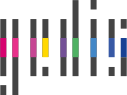
\includegraphics[scale=.45]{images/gedis_logo.png}} &
	\end{tabularx}

	\vspace{2.5cm}

	\begin{center}
 
		% Title and subtitle
		\huge{\thesistitle}

		\vspace{3cm}

		\renewcommand{\baselinestretch}{1.3}
		\Large{\thesistype}

		\large
		\thesistypedesc
	\end{center}

	\vspace{1.5cm}
	\renewcommand{\baselinestretch}{1}
	\begin{table}[htpb]
		\centering
		\begin{tabular}{ll}
			\\
			Eingereicht von: & \thesisauthorname \\
			Anschrift: & \thesisauthorhomestreet \\
			& \thesisauthorhometown \\
			\\
			Matrikelnummer: & \thesisauthormatrikelnumber \\
			E-Mail: & \thesisauthoremail \\
			\\
			Vorgelegt im: & \thesisdepartment \\
			\\
			Prüferin: & \thesisfirstreviewer \\
			\\
			Eingereicht am: & \thesisdate \\
		\end{tabular}
	\end{table}

	% font with serifs
	\rmfamily
\end{titlepage}


    \chapter*{Persönliche Anmerkung}\addcontentsline{toc}{chapter}{Persönliche Anmerkung}

Bevor Sie mit dem Lesen dieser Semesterarbeit beginnen, möchte einige im Folgenden getroffene Entscheidungen erklären.
Des öfteren enthält dieses Dokument gekürzte Fassungen der eigentlichen Beobachtungen oder Arbeitsschritte, was ich zu entschuldigen bitte.
Dies resultiert aus dem enormen Umfang des gewählten Kontextes, welcher mit meiner zur selben Zeit stattfindenden Projektarbeit zusammenhängt.
Der Vorgang der Datenerhebung ist in dieser Arbeit somit vollständig außen vor gelassen.
Es wird sich einzig auf die im Moment einer Durchsuchung auftretenden Tätigkeiten konzentriert.
Jedoch musste auch dieser Teil an einigen Stellen gekürzt werden.
An betreffenden Stellen wird dies gesondert erwähnt.

Trotz dieser Einschränkungen und Kürzungen übersteigt das Dokument bei weitem den geforderten Umfang.
Eine weitere Kürzung der Inhalte hätte jedoch einen deutlichen Qualitätsverlust in Form einer Nichtabdeckung aller geforderten Inhalte, bzw. einer Nichtabdeckung des vollständigen nutzungsorientieren Prozesses nach sich gezogen, weshalb ich mich schlussendlich dazu entschieden habe, dieses Dokument in seiner jetzigen Länge abzugeben.

    \tableofcontents

    \pagebreak
    \pagenumbering{arabic}

    % Hier Kapitel einfügen
    \chapter{Einleitung}\label{ch:einleitung}

Dieses Dokument beinhaltet eine Dokumentation der exemplarischen Umsetzung des Prozesses der nutzungsorientierten Gestaltung am Beispiel des "Digitalen Meldekopfes" des Finanzamts Kassel. 
Es entsteht im Rahmen der Veranstaltung "Nutzungsorientierte Gestaltung" an der Universität Kassel im Wintersemester 2022 - 2023 als abschließende Semesterarbeit.

Hierzu wird der nutzungsorientierte Prozess einleitend beschrieben, sowie der gewählte Kontext und die daraus resultierenden Aufgaben vorgestellt.
Nach Vorstellung einiger im Zuge des Prozesses zur Anwendung kommenden Tools wird mit Hilfe derer der Ausgangszustand des Kontextes erhoben.
Aufbauend auf diesem wird ein Soll-Zustand erarbeitet und genauer vorgestellt.
Dieses Konzept wird darauf folgend durch Rückmeldungen von im Kontext tätigen Personen angepasst und verbessert.
Abschließend folgt eine Reflektion des Prozesses und des daraus entstandenen Produkts.

Die Arbeit orientiert sich in vielen Teilen direkt an den, die Vorlesung "Nutzungsorientierte Gestaltung" begleitenden, Materialien \cite{NOG} und hat auf Grund ihres Umfangs keines Wegs Anspruch auf völlige Widerspiegelung des Erlernten.
Die Folgende Ausarbeitung ist als stark komprimierte Wissenswiedergabe mit anschließender praktischen Anwendung zu verstehen.

        \section{Hinführung}

In diesem Abschnitt werden die Lesenden in das Thema nutzungsorientierte Gestaltung eingeführt.
Hierzu wird der Begriff definiert, wichtige Aspekte der nutzungsorientierten Gestaltung herausgestellt und ihr Ablauf beschrieben.
Schlussendlich wird auf die Wichtigkeit der nutzungsorientierten Gestaltung für die Informatik eingegangen.

\subsection{Definition}\label{sec:definition}

Das traditionelle Vorgehen in der Softwareentwicklung ist es, von der Technik hin zum Menschen zu denken.
Dies ist für viele Entwickelnde einfach, da das entstehende Produkt so im Laufe des Entwicklungsprozesses an die verfügbare Technik angepasst werden kann.
Nutzungsorientierte Gestaltung (NOG) bricht mit dieser Vorgehensweise.

\begin{quote}
User-Centered Design (hier: Nutzungsorientierte Gestaltung, Anm.d.Auth) ist ein Konzept der Produktentwicklung und -gestaltung, das die Nutzerbedürfnisse in den Mittelpunkt des Entwicklungsprozesses rückt, um ein eine optimale User Experience zu ermöglichen. \cite{IONOS_nog_def}
\end{quote}

Zu erkennen ist, dass NOG die Nutzenden der Software schon bei der Entwicklung in den Mittelpunkt stellt.
Hierfür muss ein entwickeltes System Funktionen bereitstellen, welche den Arbeitsalltag erleichtern und nicht nur ihre technischen Anforderungen erfüllen.
Es soll also "verständlich, handhabbar, erlernbar [und] intuitiv" \cite{NOG} sein. 
Dies kann durch Usability Engineering, sowie dem Fokus auf Benutzerschnittstellen und der Mensch-Maschine Interaktion erreicht werden.
Hierbei gilt es einige Kriterien einzuhalten:

\textbf{Aufgabenangemessenheit} sieht vor, dass die entstehende Software genau dem Problem angemessen ist.
Dabei soll sie alle benötigten Funktionen enthalten, darüber hinaus aber keine weitere, für die Nutzenden störende oder verwirrende, Funktionen besitzen.
Es weiteren wird versucht die Anzahl an Mensch-Maschine Interaktionen auf ein Mindestmaß zu reduzieren.

\textbf{Selbstbeschreibungsfähigkeit} verlangt vom System, dass Nutzende das System ohne längere Einführung durch Dritte sofort nutzen und verstehen können.
Dazu können System eigene Hilfen und Rückmeldungen implementiert werden.

\textbf{Lernförderlichkeit} liegt in direktem Zusammenhang zur Selbstbeschreibungsfähigkeit.
Bei größeren Systemen für komplexere Anwendungsfälle ist eine vollständige Selbsterklärung der Systeme nur schwer möglich.
Trotzdem sollen Systeme den Lernprozess unterstützen.
Beispielsweise kann eine Software, wie bei Videospielen üblich, über ein Tutorial zum Erlernen dieser verfügen.

\textbf{Steuerbarkeit} bedeutet, dass die Mensch-Maschine Interaktion durch die Nutzenden initiiert werden soll.
Diese müssen zu jedem Zeitpunkt das System steuern.
Dieses darf keine unerwarteten, eigenen Aktionen durchführen.

\textbf{Erwartungskonformität} bezieht sich auf das verhalten den Systems.
Dieses soll an das erwartete Verhalten der Nutzenden angepasst werden, wobei auch stark der Nutzungskontext beachtet werden muss.
Ebenso ist eine konsistente Gestaltung der Funktionen wichtig.

\textbf{Fehlertoleranz} erlaubt es den Nutzenden trotz nicht vermeidbarer Eingabefehler weiterhin eine gute bis optimale Experience zu erlangen.
Dafür muss das System die Nutzenden entweder auf Fehler aufmerksam machen oder, sollten diese unentdeckt bleiben, ohne fatale Fehler mit den Eingaben arbeiten können.

\textbf{Individualisierbarkeit} ermöglicht es den Nutzenden das System genau für ihren konkreten Arbeitskontext anzupassen. 
Da sich dieser von Situation zu Situation andern kann, soll diese Individualisierbarkeit leicht zugänglich und umzusetzen sein.

NOG ist also mehr als nur Oberflächengestaltung.
Deshalb beinhaltet der nutzungsorientierte Prozess multi-disziplinären Aspekte von Design, Softwareentwicklung und Sozialwissenschaften.

Diesen Aufwand belohnt NOG durch eine Qualitätsverbesserung, Akzeptanzerhöhung und gleichzeitig eine, durch die Einbindung der Nutzenden resultierende, Vermeidung technischer Fehlentwicklungen.

\subsection{Prozessablauf}\label{sec:prozessablauf}

NOG ist als Kreislauf aus Verstehen, Definieren, Gestalten und Evaluieren zu verstehen.
Dieser Kreislauf wird viele Male durchlaufen, bis am Ende ein den nutzungsorientieren Anforderungen entsprechendes Resultat entsteht.

Der Ablauf des nutzungsorientierten Prozesses ist in \autoref{fig:nog_process} als linearer Prozess zu sehen.
Im Folgenden wird dieser genauer beleuchtet und aufgezeigt, an welchen Stellen sich dort der soeben benannte Kreislauf auffinden lässt.
Die im Zuge dieser Auflistung erwähnten Methoden werden unter \autoref{sec:methoden} genauer erklärt.

\begin{figure}[htp]
    \centering
    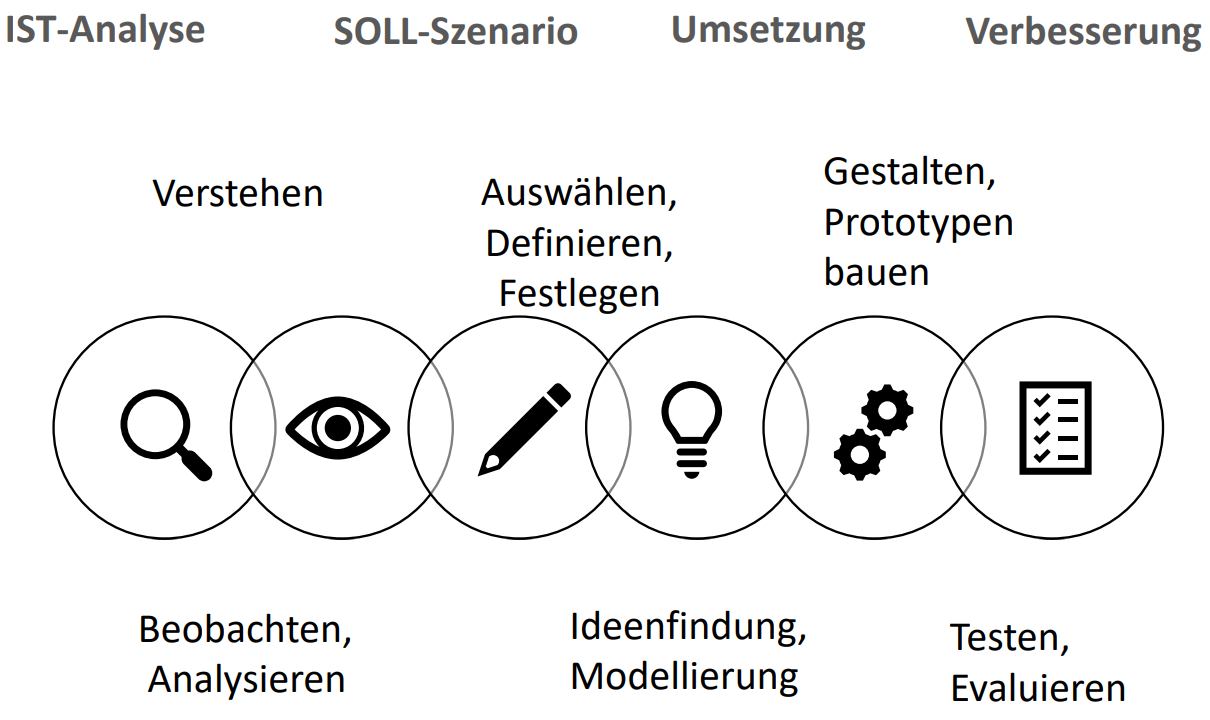
\includegraphics[width=1\textwidth]{images/NOG_Prozess.png}
    \caption{Ablauf des nutzungsorientierten Prozesses}
    \label{fig:nog_process}
\end{figure}

\autoref{fig:nog_process} verwendet für den oben benannten Kreislauf die Begriffe IST-Analyse, SOLL-Szenario, Umsetzung und Verbesserung. 
Diese Vorgänge seien nun aufgelistet und beschrieben.

\subsubsection{IST-Analyse}

In diesem ersten Abschnitt der NOG geht es darum, den vorherrschenden Kontext zu verstehen.
Dies ist essenziell um nutzerzentrierte Software zu entwickeln.
Um die Tätigkeiten und Abläufe des Kontextes zu verstehen, wird zunächst Kontakt zu Personen aus dem konkreten Nutzungskontext aufgenommen.
Mit einer oder mehreren dieser Personen wird ein Interview im Kontext durchgeführt.
Eine Erläuterung dieser Methode ist \autoref{sec:interview} zu entnehmen.
Ebenso werden zu diesen Zeitpunkt Contextual Design Modelle herangezogen, damit weiter in den Kontext eingestiegen werden kann und dieser besser verstanden wird.
Eine Erläuterung zu Contextual Design Modellen ist in \autoref{sec:modelle} zu finden.

Auf Basis der erlernten Informationen über den Kontext werden sodann sogenannte Personas, fiktive, den typischen zukünftigen Nutzenden der Software entsprechenden, Personen erstellt.
Eine Erläuterung des Konzepts der Persona findet sich in \autoref{sec:persona}.
Schlussendlich werden ein oder mehrerer IST-Szenarien verfasst, welche die vorherrschenden Abläufe des Kontextes, durchgeführt durch die zuvor erstellten Personas, zusammenfasst.
Auch eine Erläuterung zu Szenarios ist im Folgenden zu finden.
Sie ist \autoref{sec:sezenarien} zu entnehmen.

\subsubsection{SOLL-Szenario}

Im zweiten Schritt der NOG soll auf Basis der IST-Analyse ein SOLL-Szenario erarbeitet werden. 
Dieses SOLL-Szenario, beziehungsweise diese SOLL-Szenarien, basieren auf den IST-Szenarien.
Nun verfügen die Handelnden jedoch über die zu entwickelnde Software als Hilfestellung für ihre Tätigkeit.
Bei der Erstellung dieser Szenarien ist darauf zu achten, dass die Aspekte der NOG eingehalten werden.
Sie bilden das Fundament für die weitere Entwicklung der Software.

\subsubsection{Umsetzung}

Dieser dritte Schritt im Prozess der NOG nutzt die gesammelten Informationen und Ideen der IST- und SOLL-Analysen um darauf aufbauend einen Prototyp für das fertige Produkt zu erstellen.
Diese Prototypen können in verschiedenen Formen erstellt werden.
Weitere Infos hierzu ist \autoref{sec:prototypen} zu entnehmen.
Auch hierbei ist, sogar noch intensiver als im Zuge der SOLL-Szenarien, darauf zu achten, dass alle Prinzipien und Aspekte der NOG eingehalten werden.

\subsubsection{Verbesserung}

In diesem Schritt wird die bisher geleistete Arbeit den Kontextpersonen vorgestellt.
Damit diese einen möglichst guten Einblick in die Ideen und Lösungen der Entwickelnden haben, müssen letztere so realistische Prototypen wie möglich erarbeiten.
Nach einer Vorstellung der Prototypen können die Kontextpersonen Rückmeldungen über das erarbeitete Konzept geben.
Je nach Art des Prototypen kann dieser auch praktisch im Kontext erprobt werden.

Mit der Rückmeldung der Kontextpersonen schließt sich der am Anfang des Kapitels angesprochene Kreis der NOG.
Die Entwickelnden begeben sich mit dem aus den Rückmeldungen gewonnen Wissen zurück zum Schritt des SOLL-Szenarios oder der Umsetzung, damit die gewünschten Änderungen dort eingearbeitet werden können.
Diese iterative Entwicklung des Produkts hält an, bis dieses dem Anspruch und Nutzen der Nutzenden gewachsen ist.

\newpage
\subsection{Wichtigkeit}

Zum Schluss dieses Abschnittes sei noch einmal die Wichtigkeit von nutzungsorientierter Gestaltung für die Informatik betont.
Bereits zu Beginn wurde erwähnt, dass der traditionelle Ansatz der Softwareentwicklung von der Maschine hin zum Menschen arbeitet.
Da die Software jedoch am schlussendlich von Menschen verwendet werden soll, hat dieser Ansatz nicht den besten praktischen Nutzen.
Ein auf diese zugeschnittenes digitales System kann nicht nur das Wohlbefinden, sondern auch die Produktivität der Nutzenden steigern \cite{NOG}.
Ein weiterer Vorteil der Einbindung von Nutzenden in die Entwicklung der Software ist, dass diese dem Resultat offener gegenüber stehen.
Oft haben Personen, welche längere Zeit eine Tätigkeit auf die selbe Weise ausführen keine Toleranz für (technische) Änderungen an ihren Arbeitsabläufen.
Arbeiten diese Personen jedoch direkt an der zu verwendenden Technik mit, so so reduziert sich diese Barriere auf ein Minimum.
        \section{Kontext}

Dieser Abschnitt definiert den in diesem Dokument bearbeiteten Nutzungskontext, den (Digitalen) Meldekopf des Finanzamts Kassel.
nach Erläuterung der Motivation folgt eine Übersicht über das Finanzamt Kassel, sowie die Tätigkeiten eines Meldekopfes.

\subsection{Motivation}

Anfang November 2022 sollten Kontexte für eine exemplarische Durchführung des Prozesses der NOG gefunden werden.
Der Autor ist als dualer Student beim Finanzamt Kassel beschäftigt und bearbeitet zur Zeit ein Semesterprojekt am Fachgebiet Software Engineering der Universität Kassel in Kooperation mit dem Finanzamt Kassel. 
Dabei handelt es sich um die Digitalisierung der Einsatzzentrale von Großdurchsuchungen der Steuerfahndung Kassel.
Zur Zeit der Kontextwahl befand sich dieses Projekt in der Phase der Anforderungsfindung.
Somit bot es sich an, den Inhalt des Semesterprojekts auch auf die Veranstaltung "Nutzungsorientierte Gestaltung" zu übertragen.

Da das Finanzamt Kassel sensibel Daten verarbeitet, sind dies betreffende Inhalte im Folgenden teilweise aus Gründen der Diskretion gekürzt, abgeändert oder geschwärzt.

\subsection{Meldekopf}

Das Finanzamt Kassel ist das nördlichste der 47 hessischen Finanzämter.
Unter anderem in Kassel angesiedelt ist die Steuerfahndung für Nordhessen.
Einige Male im Jahr führt diese größere Durchsuchungsmaßnahmen durch, für welche eine zentrale Organisation, eine Einsatzzentrale, von Nöten ist.
Diese Einsatzzentrale oder auch Meldekopf besteht aus mehreren Personen, welche mit Hilfe von Papier Unterlagen und Telefonaten die Durchsuchungen der verschiedenen Objekte organisieren.

Das Vorbereiten und Organisieren von Großdurchsuchungen ist der Kontext der hier vorgestellten Durchführung des nutzungsorientierten Prozesses.
Dabei soll die Notwendigkeit von Papier Unterlagen auf ein Minimum reduziert werden, sowie die Übersichtlichkeit der aktuellen Situation verbessert werden.
Des weiteren soll ein integriertes Protokolliersytem eingeführt werden, welche des der Behörde erlaubt, den Ablauf einer Durchsuchungen im Nachhinein genau nachzuvollziehen. 
Auf weitere Ideen und Konzepte des Produkts, welche im Zusammenhang mit NOG stehen wird im weiteren Verlauf dieser Arbeit eingegangen.
        \section{Personen und Tätigkeit}

Dieser Abschnitt stellt den Lesenden die im nutzungsorientierten Prozess beteiligte, im Kontext tätige Person, sowie ihre Tätigkeiten vor.
Dabei wird ein Fokus auf die zu optimierende Aufgabe, dem Organisieren und Durchführen von Großdurchsuchungen im Meldekopf, gelegt.
Zu beachten ist, dass aus Gründen der Diskretion der Name der erwähnten Person geändert wurde.

\subsubsection{Kontextperson}

Als Kontextperson, beziehungsweise Ansprechperson aus dem Kontext, steht Hannah Christensen zur Verfügung.
Frau Christensen arbeitet seit vielen Jahren in der hessischen Finanzverwaltung und ist zur Zeit in der Steuerfahndung Kassel eingesetzt.
Dort betreut sie des öfteren größere Fallkomplexe, für deren Abschluss Großdurchsuchungen nötig sind.
Die Momentanen Abläufe für das Vorbereiten und Organisieren wurden vor einiger Zeit von Frau Christensen entwickelt, trotzdem ist sie an einer Digitalisierung des Meldekopfs interessiert.

\subsubsection{Fokussierte Tätigkeit}

Bearbeitet Frau Christensen einen Fallkomplex welcher eine Großdurchsuchung benötigt, so ist sie verantwortlich diese vorzubereiten, jedoch nicht den Meldekopf dieser Durchsuchung zu übernehmen.
Nach vollendeter Durchsuchung werden ihr ein Protokoll des Meldekopfes, sowie die sichergestellten Unterlagen übermittelt, welche sie daraufhin auswertet.
Im Zuge des benannten Kontextes nimmt Frau Christensen also die Aufgabe des Vorbereitens der Durchsuchung war.
Die Organisation im Meldekopf wird von immer wechselnden Kollegen durchgeführt.
Auch Frau Christensen saß bereits bei Durchsuchungen anderer KollegInnen im Meldekopf.

    \chapter{Eingesetzte Methoden}\label{sec:methoden}

Dieses Kapitel behandelt und beschreibt die in der nutzungsorienterten Gestaltung genutzten Tools und Methoden.
Diese wurden in Teilen bereits im Zuge des Prozessablaufes in \autoref{sec:prozessablauf} erwähnt.

Die hier aufgeführten Methoden bilden das Fundament für eine erfolgreiche Ausarbeitung im Sinne der nutzungsorientierten Gestaltung.
Ebenso sind sie Grundlage für die folgenden Kapitel \hyperref[sec:anwendung]{IST-Analyse}, \hyperref[sec:gestaltung]{SOLL-Zustand}, \hyperref[sec:feedback]{Anpassungen} und \hyperref[sec:incdes]{Inclusive Design}.

Die verwendeten Definitionen sind dem Inhalt der Vorlesung "Nutzungsorientierte Gestaltung" \cite{NOG} entnommen.
        \section{Interview im Kontext}\label{sec:interview}

Das Interview im Kontext ist eine Methode, mit welcher die Entwickelnden Informationen über den aktuellen Zustand in einem Kontext bekommen können.
Entwickelt wurde es in der Mitte der 1990er Jahre von Holzblatt und Beyer erfunden \cite{InterviewIK}.
Ziel es Interview ist es, auf Basis von konkreten Arbeitssituationen der Nutzenden, zuverlässige und umfangreiche Daten über den Einsatz, die Nutzung und den Kontext von IT zu erheben.
Dabei wird das existierende System in Bezug auf Beziehungen, Abläufe, Widersprüche, Fehler und Überflüssigkeiten genauestens untersucht.
Ebenso entwickelt sich durch das Interview im Kontext ein Bild der Gruppe der Nutzenden, welches später beim Erstellen von Personas wichtig wird.

Das Interview im Kontext ist ein Beobachtungsinterview.
Informationen werden also nicht vorrangig durch Fragen, sondern durch Beobachtungen gewonnen.
Dabei befinden sich die Interviewenden in der Rolle eines Lehrlings, während die Kontextperson die Rolle eines Meisters einnimmt.
In dieser Rolle begleiten die Interviewenden die Kontextperson bei ihren Tätigkeiten im Kontext.
Eine detaillierte Ablaufbeschreibung des idealen Interviews im Kontext ist \autoref{ap:checkliste} zu entnehmen.
Diese kann jedoch auf den vorherrschenden Kontext angepasst werden.
Ein Beispiel einer Anpassung ist im weiteren Verlauf dieser Arbeit unter \autoref{sec:interview-praktisch} zu finden.
Über das Beobachten der Kontextpersonen sind Fragen der Interviewenden möglich.
Diese sollen jedoch konkret und nicht abstrakt formuliert werden, damit das Interview weiter so nah wie möglich an einer konkreten, realen Aufgabe stattfindet.
Des Weiteren sollen sich die Beobachtenden durch Bescheidenheit, Neugier und Aufmerksamkeit auszeichnen.

Das Interview im Kontext folgt den Grundprinzipien Kontext, Partnerschaft, Interpretation und Fokus.
Diese seien im Folgenden näher beleuchtet.

\subsection{Kontext}

Die Interviewenden müssen zu jeder Zeit des Interview den Kontext im Bezug halten.
Dabei sollen die gewonnenen Erfahrungen als laufende und nicht als zusammengefasste Erfahrungen analysiert werden.
Des Weiteren gilt es, stehts nah an realen Abläufen zu agieren und nicht an fiktiven, möglicherweise nicht die Realität , Abläufen zu arbeiten.
Es muss also ein Fokus auf Konkretem und nicht auf Abstraktem liegen.
Ebenso sollen die Interviewenden stehts zum Weiterarbeiten anregen und mit gezielten Fragen den Kontext der aktuellen Aufgabe erfassen.
Hier kann beispielsweise nach dem Grund für die Aufgabe oder einem ähnlichen Fall und dessen Ausgang gefragt werden.

\subsection{Partnerschaft}

Dieses Prinzip stellt die Zusammenarbeit zwischen den Interviewpartnern heraus.
Es sei wiederholt, dass das Interview im Kontext nicht mit der traditionell in einem Interview herrschenden Marktsituation übereinstimmt.
Die Kontextperson entscheidet, wann und wie lange über ein Thema geredet wird.
Dieses Privileg ist dieser vor dem Interview klar mitzuteilen.

Diese Unterordnung der Interviewenden hat einige Gründe:
Es soll verstanden werden, wie die Arbeit unterstützt werden kann.
Hierzu ist es essentiell, dass diese Arbeit zunächst ungefiltert betrachtet wird.
Dies ist nur möglich, wenn die Kontextperson in der Machtposition ist.
Ebenso werden gewisse Arbeitsaspekte unterbewusst ausgeführt.
Um diese wahrnehmen zu können, muss die Kontextperson nach eigenem Ermessen handeln können und ihre Aufgaben wie gewohnt erledigen.

Im Idealfall sollten die Interviewenden Fragen steht nach Beendung eines Arbeitsschritts stellen.
So wird auch die Kontextperson zum Reflektieren angeregt, was dazu führen kann, dass diese mehr Informationen explizit an die Interviewenden weitergeben kann.

\subsection{Interpretation}

Der Punkt der Interpretation wird nach dem Interview im Kontext wichtig.
Die Interviewenden müssen darüber im Klaren sein, dass sie subjektive und nicht objektive Beobachtungen gesammelt haben.
Diese müssen unter dem Aspekt der Subjektivität beurteilt werden.

Nach abgeschlossener Interpretation des Interviews sind die Ergebnisse mit der Kontextperson abzugleichen.
Diese erkennt mögliche Missinterpretation und kann diese klarstellen.
Wichtig ist, dass Design-Ideen als letztes Glied dieser Bildung von Verständnis gesehen werden sollen.
Es sollen also nicht im Zuge des Interviews direkt Ideen an die Kontextperson weitergegeben werden.

\subsection{Fokus}

Als letztes Prinzip ist Fokus zu nennen.
Hierbei geht es nicht um den Grad der Aufmerksamkeit, sondern deren Ziel.
Wichtig ist es, den Fokus auf Unerwartetes zu legen.
Als Außenstehender ist es schwer, Ausnahmen von regulären Arbeitsschritten zu unterscheiden.
Für diese Fälle sind Nachfragen geeignet.
Es muss darauf geachtet werden, dass das der Fokus nicht auf der Bestätigung der eigenen Auffassung liegt, sondern, dass die Interviewenden offen für Überraschungen und Widersprüche sind.

        \section{Personas}\label{sec:persona}

Personas erhalten ihren Namen von den gleichnamigen Masken antiker Schauspieler.
Entwickelt wurden sie Ende der 90er Jahre von Alan Cooper \cite{PersonaCooper}.
Personas sind fiktive Personen, welche die durchschnittlichen Nutzenden widerspiegeln sollen.
Eine Persona ist somit nie von einer konkreten Person inspiriert, mehr von einer Gruppe an Personen.
Im Normalfall werden im Zuge des nutzungsorientierten Prozesses einige wenige Personas erstellt, welche zusammen einen möglichst großen Teil der Nutzenden abdeckt.

Personas ermöglichen es den Entwickelnden für konkrete Personen zu entwickeln.
Dies ist hilfreich, wenn über die Umsetzung eines Features diskutiert wird.
Hier kann überlegt werden, ob die Persona dieses Feature hilfreich findet.
Das Argument "Irgendjemand will doch sicher..." ist somit hinfällig.
Es ist auch möglich, eine Persona zu erstellen, welche das Gegenteil der Nutzenden verkörpert und gegen welche das System ausgerichtet wird.

\begin{figure}[htp]
    \centering
    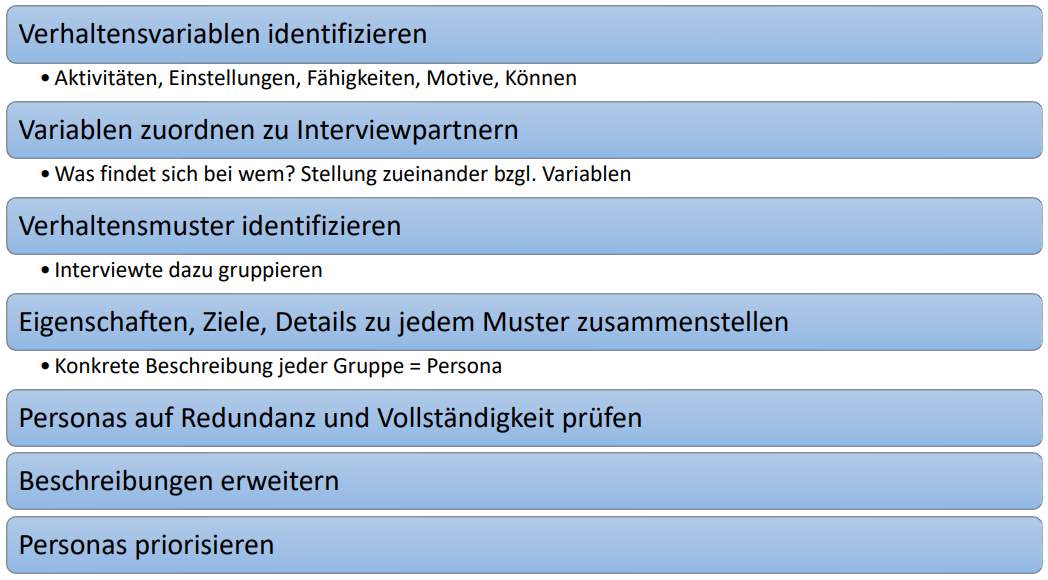
\includegraphics[width=\textwidth]{images/Persona-Leitfaden.png}
    \caption{Leitfaden zum Erstellen von Personas}
    \label{fig:personaLeitfaden}
\end{figure}

Da Personas Nutzende verallgemeinern ist zu beachten, dass hier häufig Stereotypen entstehen.
Bei der Erstellung ist es somit wichtig, nicht auf Vorurteile zurück zufallen.
Sollten mehrere Personas entwickelt werden, so ist zu beachten, dass diese eine möglichst kleine Überschneidung in ihren Merkmalen haben sollen.
Ziel ist es, auf effiziente Weise mit so wenig Personas wie möglich einen möglichst großen Raum der Nutzenden abzudecken.

Personas sollen erlebbar sein.
Hierzu ist es wichtig, diese auch über die für den Kontext wichtigen Attribute zu entwerfen.
Personas haben praktische und persönliche Ziele, betreiben bestimmte Aktivitäten, haben Hobbys und Einstellungen, sowie personalisierte Fähigkeiten, Wissen und Erfahrungen.
Ebenso soll ihre Herkunft, Bildung, Aussehen und ihre Familienbeziehung klar aus der Beschreibung hervor gehen.

Personas werden aus empirischen Erhebungen erstellt.
Hierzu kann einem Leitfaden gefolgt werden.
Dieser ist von Cooper, Reimann und Cronin \cite{PersonaCooperEtA} entwickelt worden und in \autoref{fig:personaLeitfaden} zu sehen\footnote{Konzept von Cooper, Reimann und Cronin aus \cite{PersonaCooperEtA}, Darstellung aus \cite{NOG}}.

Die Darstellung einer Persona kann unterschiedlich sein.
Sie kann auf Papier gezeichnet werden, in einem Text beschrieben werden oder auch grafisch dargestellt werden.
Einige Beispiele von Personas sind im Anhang unter \autoref{ap:personas} zu finden. 
Darüber hinaus ist in \autoref{fig:personaPaul} eine Persona für den hier praktisch behandelten Kontext zu finden.
        \section{Contextual Design Modelle}\label{sec:modelle}

Contextual Design Modelle sollen die Erfassung des Kontextes weiter vereinfachen.
Hierzu gibt es eine Vielzahl verschiedener Modelltypen.
Diese können digital, aber auch physisch vorliegen.
Auch können verschiedene Modelltypen kombiniert werden.
Im Folgenden seien die in \cite{NOG} besprochenen Modelltypen aufgelistet und kurz beschrieben.
Zu diesen sind jeweils Beispiele aus der Gebäudetechnik der Universität Bremen gegeben.
Diese sind \cite{NOG} entnommen.

\subsection{Flussmodell}

Ein Flussmodell ist als ein gerichteter Graph zu verstehen.
Dabei sind die Knoten Gegenstände, Räume oder Personen.
Die Kanten stellen Tätigkeiten oder andere Leistungen der Objekte dar.
Knoten können in ihrer Darstellung variabel sein
Beispielsweise können Personen als Ellipsen und Räume als Rechtecke dargestellt werden.

\begin{figure}[htp]
    \centering
    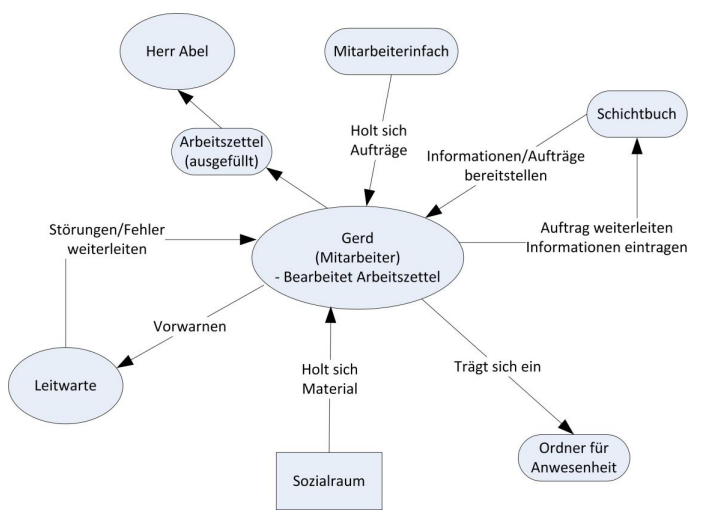
\includegraphics[width=.7\textwidth]{images/3-Modelle/flussmodell.png}
    \caption{Beispiel Flussmodell aus \cite{NOG}}
    \label{fig:flussmodell}
\end{figure}

\autoref{fig:flussmodell} die Abläufe der Gebäudetechnik der Universität Bremen als Flussmodell.
Aus einem Flussmodell sind schnell grobe Abläufe und Abhängigkeiten zu erkennen.
Dies ist nützlich, wenn ein Bild des gesamten Kontextes benötigt wird.
Informationen sind hier jedoch abstrakt und nicht konkret an einem Beispielszenario gezeigt.
Es ist also zu empfehlen, zusätzlich zu einem Flussmodell ein weiteres, konkretes Modell heranzuziehen.

\subsection{Sequenzmodell}

Sequenzmodelle stellen konkrete Abläufe in detaillierten atomaren Schritten dar.
Dabei wird zu jedem Schritt ein Zweck, die Handlung und mögliche Störfälle notiert.
Sequenzmodelle können auch die Erfahrungen mehrerer Ausführungen einer Tätigkeit enthalten.
Dies ist im in \autoref{fig:sequenzmodell} zu sehenden Modell der Fall.

\begin{figure}[htp]
    \centering
    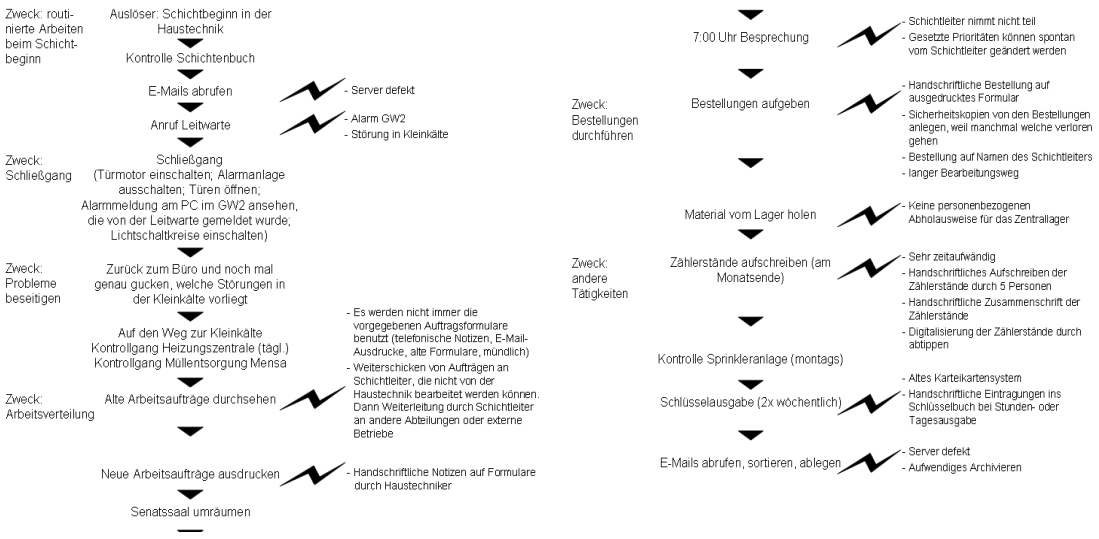
\includegraphics[width=\textwidth]{images/3-Modelle/sequenzmodell.png}
    \caption{Beispiel Sequenzmodell aus \cite{NOG}}
    \label{fig:sequenzmodell}
\end{figure}

In diesem wurde ein Haustechniker mehrere Tage bei seiner morgendlichen Routine begleitet.
Die daraus gewonnenen Eindrücke und Informationen wurden mit Hilfe eines Sequenzmodells dargestellt.
Dieses Modell ist nützlich, wenn konkrete Abläufe detailliert betrachtet werden sollen.
Es eignet sich jedoch nicht, um einen größeren Kontext in seiner Gesamtheit zu erfassen.

\subsection{Kulturelles Modell}

Kulturelle Modelle spiegeln das soziale Umfeld des Kontextes wider.
Es ist ähnlich wie ein Flussmodell aufgebaut.
Die Kanten stehen nun jedoch für kulturelle und soziale Ansichten.
Diese können auch in Form von Zitaten an die Kanten geschrieben werden.
Ebenso ist es möglich, mehrere Ansichten an einer Kante anzufügen.

Kulturelle Modelle sind geeignet, damit der soziale Kontext der Kontextpersonen betrachtet werden kann.
Es hilft, wenn Beziehungen zwischen verschiedenen Individuen im Kontext untersucht werden sollen.

\subsection{Physikalisches Modell}

Physikalische Modelle spiegeln den räumlichen Kontext wider.
Aus ihnen ist zu erkennen in welchem Gebiet und Umfang sich die Nutzenden während der Ausführung ihrer Aufgaben bewegen müssen.
Diese Modelle können im zweidimensionalen Raum, aber auch als dreidimensionale Modelle ausgeführt werden.
Wichtig ist jedoch, dass die Wege oder Arbeitsplätze der Nutzenden aus diesen Modellen erkenntlich sind.
Nicht erweiterte Grundrisse stellen hier kein echtes physikalisches Modell dar.

\begin{figure}[htp]
    \centering
    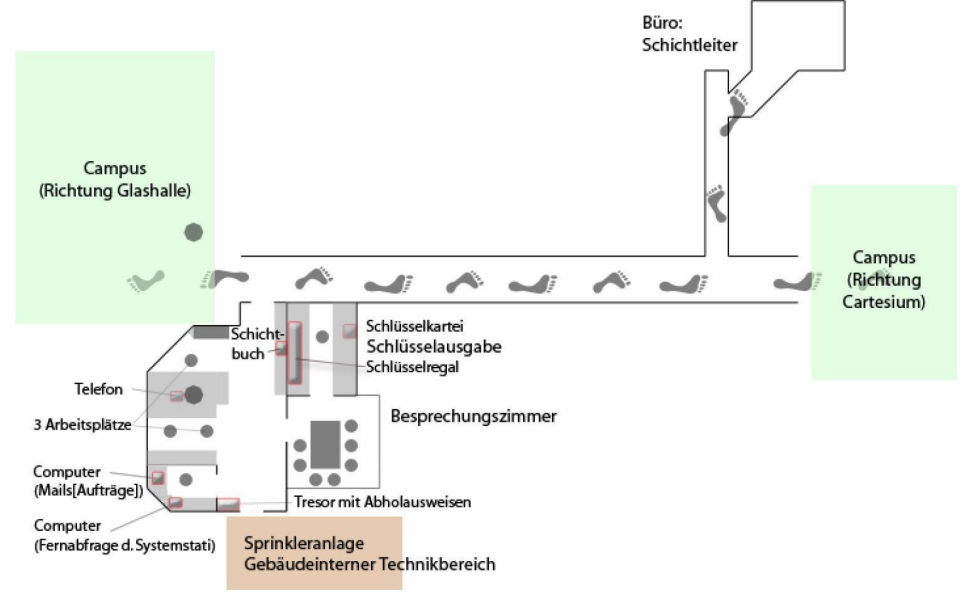
\includegraphics[width=.75\textwidth]{images/3-Modelle/physikalischesmodell.png}
    \caption{Beispiel Physikalisches Modell aus \cite{NOG}}
    \label{fig:physikalischesModell}
\end{figure}

\autoref{fig:physikalischesModell} zeigt ein physikalisches Modell der Aufgaben eines Haustechnikers der Universität Bremen.
Aus ihm sind sowohl der Arbeitsplatz der Haustechniker, also auch deren Wege im Gebäude ersichtlich.
Darüber hinaus wurden wichtige Orte und Objekte in der zweidimensionalen Ansicht markiert.

\subsection{Artefaktmodell}

Als Artefaktmodelle sind sämtliche Dokumente oder Gegenstände benannt, welche dem Nutzungskontext entstammen.
Sie helfen, wenn der Einsatz von Medien genauer untersucht werden soll.
Im Falle der Haustechnik kann hier beispielsweise ein Schichtbuch oder eine Schlüsselkarte, welche das Ausleihen von Schlüsseln dokumentiert, herangezogen werden.
Artefaktmodelle werden im Gegensatz zu den bisher kennengelernten Modellen nicht von den Entwickelnden, sondern von den Nutzenden erstellt und zur Verfügung gestellt.

\subsection{Culture Probes}

Culture Probes können ähnlich wie Artefaktmodelle gesehen werden, werden jedoch nicht vorgefunden, sondern wissentlich von den Nutzenden erstellt.
Hierzu werden den Nutzenden Hilfsmittel zur Verfügung gestellt, mit denen sich während der Ausführung ihrer Tätigkeiten agieren können.
Hier kann es sich um Zettel und Stift, aber auch eine Kamera handeln.

Bei der Auswertung von Culture Probes ist entstandenes Material nach Tätigkeiten zu Gruppieren.
Es ist somit wichtig, dass erkenntlich ist, aus welcher Tätigkeit ein erstelltes Artefakt entstammt.
        \section{Szenarien}\label{sec:sezenarien}

Szenarien werden verwendet, um konkrete Situationen textuell zu beschreiben.
Dabei können real Beobachtete Situation beschrieben werden.
Es können jedoch auch ideale Situationen in Form von SOLL-Szenarien erstellt werden.

IST- und SOLL-Szenarien folgen einem gemeinsamen Leitfaden.
Sie verfügen grundlegend über einen Titel, einen Aktor und eine Aufgabenstellung.
Das Szenario beschreibt die Ausführung der Aufgabenstellung durch den Aktor.
Dabei werden Nutzungskontext, Kommunikation, Hierarchien und Herausforderungen in das Szenario eingearbeitet.
Szenarien sollen Abläufe nicht bewerten.
Ihr Ziel ist es eine möglichst neutrale Beschreibung einer Situation darzustellen.

Als Aktor der Szenarien werden in vielen Fällen bereits erstellte Personas verwendet.
Dies bietet sich an, da so sichergestellt wird, dass Handlungen innerhalb des Szenarios nicht übermäßig durch die handelnde Person beeinflusst werden, da Personas einen durchschnittlichen Nutzenden darstellen.
Szenarien müssen nicht im Fließtext vorliegen.
Es ist ebenso möglich die benannten Anforderungen Stichpunktartig oder auf andere Weise zu erfüllen.

\subsubsection{IST-Szenario}

Ein IST-Szenario spiegelt den momentanen Zustand eines Kontextes wider.
Es wird aus den im Interview im Kontext und aus Modellen gewonnenen Informationen erstellt.
Diese IST-Szenarios stellen die Grundlage für zu entwickelnde Software dar.
Im Normalfall werden im Zuge des nutzungsorientierten Prozesses mehrere IST-Szenarios erstellt.

\subsubsection{SOLL-Szenario}

Ein SOLL-Szenario gibt den idealen Ablauf einer Tätigkeit wider.
Jedes SOLL-Szenario baut im idealen Fall auf einem IST-Szenario auf, welches über optimierbare Techniknutzung verfügt.
Diese optimierte Techniknutzung steht den Nutzenden im SOLL-Szenario zur Verfügung.
Dabei muss darauf geachtet werden, dass die beschriebene neue Technik den Aspekten der NOG entspricht.
        \section{Prototypen}\label{sec:prototypen}

Prototypen werden genutzt, damit Softwarekonzepte praktisch getestet werden können.
Ihre Herstellung ist weniger aufwendig und besser adaptierbar als fertige Software.
Prototypen werden genutzt um mit Hilfe von Personas und Kontextpersonen konkrete Umsetzungsideen der Software zu testen.

Es gibt viele Varianten an Prototypen.
Im Folgenden sind die Typen "Paper Prototyp" und "Wireframe/ Mockup" genauer beleuchtet.
Es folgt eine Übersicht über weitere Prototyparten und Kriterien, mit denen ein zum Kontext passender Typ gewählt werden kann.

\subsection{Paper Prototyps}

Um einen Paper Prototyp zu erstellen, wird die überlegte Software auf Papier skizziert.
Dabei wird kein Wert auf das Design gelegt.
Wichtig sind Interaktion und Idee der Entwickelnden.
Für jede benötigte Ansicht wird ein eigener Prototyp erstellt.
Änderungen an der Oberfläche werden entweder durch einen neuen Prototypen oder zusätzliche hinzu zulegende Bausteine realisiert.
Eingabefelder können beispielsweise durch Folien mit nicht permanenten Stiften realisiert werden.

Paper Prototypen sind einfach herzustellen.
Aus diesem Grund haben Kontextpersonen eine niedrige Schwelle für Kritik und Verbesserungsvorschläge.
Diese wächst mit dem in den Prototypen investierten Aufwand.
Ebenso sind keine technischen Kenntnisse nötig, um Paper Prototypen zu erstellen.
Nutzende können im Zuge von Usability Tests direkt an ihnen mitarbeiten und ihre Kritik grafisch darstellen.

Auf Grund der niedrigen Änderungsschwelle für Paper Prototypen kann der iterative Verbesserungsprozess der Paper Prototypen jedoch in die Länge gezogen werden.
Ebenso fällt die Unterscheidung zwischen "must-haves" und "nice-to-haves" schwerer.

\subsection{Wireframes und Mockups}

Wireframes sind als digitale Paper Prototyps zu verstehen. Auch hier liegt der Fokus auf Idee und Interaktion, nicht auf Design.
Im Gegensatz zu Paper Prototyps ist die Kritikschwelle hier jedoch höher, da digitale Zeichnungen steht eine längere Entwicklungszeit suggerieren.
Dies muss im Falle von Wireframes jedoch nicht der Fall sein.
Wireframes sind statische Ausschnitte aus der zu erstellenden Software.
Ebenso wie bei Paper Prototyps werden Änderungen an der Oberfläche durch neue Wireframes dargestellt.

Aufbauend auf Wireframes existiert das Konzept von Mockups.
Unter Mockups sind Wireframes zu verstehen, welche jedoch nun auch im Thema Design ausgearbeitet sind.
Es handelt es sich hier also bereits um eine statische Version des Endproduktes.

\subsection{Weitere}

Neben den bereits benannten Prototypen gibt es eine Vielzahl weiterer Möglichkeiten der Prototypisierung.
Einige von ihnen sind \autoref{fig:prototypenUebesicht} zu entnehmen.
In der Grafik sind die Typen bezüglich den Aspekten Information, Interaktion, visuellem Design, Redaktioneller Inhalte, Branding und System bewertet.

\begin{figure}[htp]
    \centering
    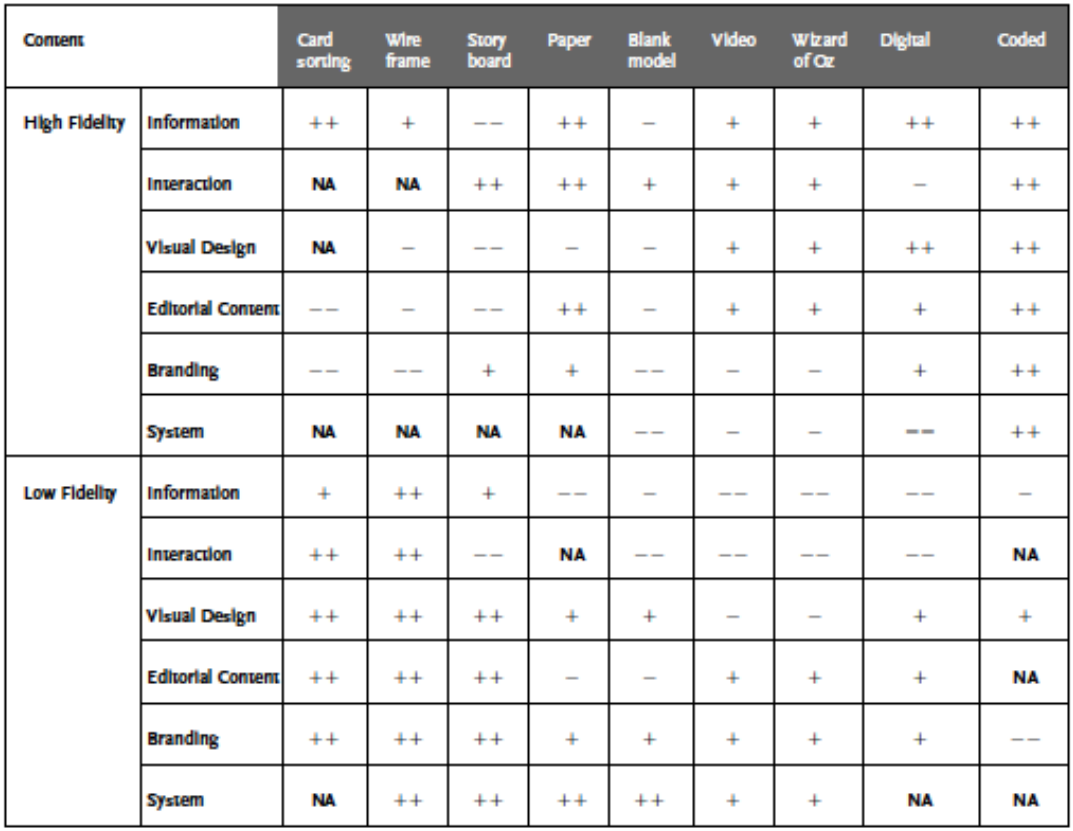
\includegraphics[width=\textwidth]{images/prototypen-übersicht.png}
    \caption{Übersicht Prototypen aus \cite{NOG}}
    \label{fig:prototypenUebesicht}
\end{figure}

Je nach Phase der Entwicklung sowie vorliegendem Kontext kann somit eine passende Art an Prototyp gefunden werden.
Die Wahl des Prototyps ist nicht auf einen einzigen beschränkt.
Mischformen oder die Verwendung mehrerer Prototypen zur selben Zeit ist möglich und in vielen Fällen auf Grund einer besseren Darstellung des Konzepts empfehlenswert.
        \section{Usability Tests}

Um das entwickelte Softwarekonzept zu testen, werden Usability Tests mit den Kontextpersonen durchgeführt.
Usability Tests lassen Kontextpersonen die Prototypen ohne direkte Hilfe der Entwickelnden testen.
Diese Tests folgen einem festen Ablauf, welcher im Folgenden erläutert wird.

\subsection{Vorbereitung}

Zunächst müssen einige Voraussetzungen für Usability Tests erfüllt werden.
Es benötigt einen ruhigen Ort, Testpersonen, sowie je einer Person zur Moderation und Protokollführung.
Die beiden letzteren müssen die Software kennen, die Testpersonen dürfen dies nicht.

Des weiteren müssen Aufgabenstellungen vorbereitet werden, welche sich nah an Beobachteten Aufgaben orientieren und einen möglichst großen Teil der Anwendung abdecken.
Diese sollen in angemessener Zeit lösbar sein und eine natürliche Abfolge an Aktionen beinhalten.
Ebenso soll ein Szenario als Rahmen des Tests vorbereitet werden.
Dies soll den Nutzenden Informationen über die Umstände geben, in denen sie die Aufgabenstellungen abarbeiten sollen.

Ebenso zu empfehlen ist ein vorausgehender Pilottest, welcher sicherstellt, dass die Aufgaben verständlich sind.
Dieser kann ebenfalls feststellen, ob große technische Probleme in der Software vorliegen oder alle Materialien zum Lösen der Aufgaben vorhanden sind.

\subsection{Durchführung}

Zu Beginn des Tests soll der Testperson klar gemacht werden, dass die Software und nicht die Benutzenden geprüft werden.
Daraufhin werden die Testpersonen gebeten, stehts geplante Aktionen und erwartete Rückmeldungen vom System zu kommunizieren.
Im Falle einer Benutzung durch mehrere Personen muss jede Aktion begründet werden.

Daraufhin werden den Testpersonen die Aufgaben und der erstellte Kontext erklärt.
Sie können daraufhin anfangen die Aufgaben zu bearbeiten.
Alle Tätigkeiten werden von der Protokoll führenden Person notiert, um diese zu einem späteren Zeitpunkt auszuwerten.
Der Moderator greift während der Bearbeitung nur im Notfall ein.
Dies könnte beispielsweise durch ein absolutes nicht Weiterkommen der Testpersonen gegeben sein.

\subsection{Nachbereitung}

Schlussendlich wird eine Nachbereitung durchgeführt.
Hier werden die Testpersonen zunächst nach ihrer grundlegenden Einschätzung des Programms gefragt.
Über diese hinaus werden Probleme, Überraschungen und Mängel besprochen und evaluiert.
Diese Diskussion wird final in einen Bericht zusammengefasst, welcher Verbesserungsvorschläge in einer konkreten, strukturierten und konstruktiven Art und Weise enthält.

    \chapter{Erfassung IST-Zustand}\label{sec:anwendung}

Dieses Kapitel umfasst die Erfassung des IST-Zustandes für den Kontext "Digitaler Meldekopf".
Auf Grund des zeitlichen Rahmens des Semesters ist nur eine Iteration des nutzungsorientierten Prozesses möglich.
Deshalb wird der Prozess der nutzungsorientierten Gestaltung hier und in den folgenden Kapiteln sequentiell bearbeitet.

Zunächst folgt ein Abschnitt über das mit Frau Christensen geführte Interview im Kontext.
Dieser besteht aus einer Dokumentation dieses Interviews und den daraus gezogenen Schlüssen.
Aufbauend auf dem Interview im Kontext und den im Zuge dessen gewonnen Informationen über die Personen im Kontext wird daraufhin eine für diese stellvertretende Persona vorgestellt.
Des Weiteren folgt die Erläuterung eines Artefaktmodelles, einem Ausschnitt aus dem Protokoll einer Großdurchsuchung.

Darauf aufbauend wird letzten Endes ein IST-Szenario verfasst, in welchem die erwähnte Persona einer gängigen Tätigkeit des Kontextes nachgeht.

        \section{Interview im Kontext}\label{sec:interview-praktisch}

Dieser Abschnitt enthält alle Informationen zum Interview im Kontext mit Frau Christensen. 
Zunächst folgt eine Dokumentation des Interviews, welche anhand von Mitschriften und Erinnerungen an dieses Gespräch entsteht.
Darauf folgt eine Auswertung des Interviews, in der Punkte herausgestellt werden, welche bei der Entwicklung eines SOLL-Zustandes berücksichtigt werden müssen.

Der Ablauf des Interviews musste in diesem Kontext leicht modifiziert werden.
Das Interview fand im Laufe einer realen Großdurchsuchung statt.
Im Zuge dieser ist stehts ein hohes Maß an Hektik präsent.
Um diese nicht weiter zu steigern, wurden Zwischenfragen zu Arbeitsschritten ans Ende der Durchsuchung verschoben.
Somit wurde zunächst über sechs Stunden eine reine Beobachtung durchgeführt.

Auf Grund der abgewandelten Durchführung des Interviews im Kontext enthält dieser Abschnitt nicht die vollständige Dokumentation der gesamten Interviewzeit.
Es werden im Folgenden also einige im Zuge der Durchsuchung beobachtete Fakten und deren Bedeutung aufgelistet.

Des Weiteren handelt es sich bei den Beobachtungen um hoch sensible Daten.
Jegliche Namen von Personen, Betrieben und weiterem müssen und sind somit geändert.
Um den Lesenden eine lebhafte Atmosphäre zu schaffen, werden Namen aus der Zeichentrick Serie \textit{SpongeBob Schwammkopf} verwendet.

\subsection{Beschreibung der physischen Umgebung}

Gegenstand der Durchsuchung ist der Verdacht auf Steuerhinterziehung in der Belegschaft der Krossen Krabbe.
Hierzu werden die Krosse Krabbe selbst, sowie die Wohnungen von Eugene Krabs, Robert Schwammkopf und Thaddäus Tentakel durchsucht.

Es ist der 22.09.2029 um 12 Uhr mittags.
Der Meldekopf sitzt in einem Besprechungsraum für ca. 20 Personen des Finanzamts Kassel.
Er besteht am heutigen Tag aus zwei Personen, Frau Vogel und Herrn Müller-Hall.
Der große Konferenztisch ist voll mit Aktenordnern, einem Notebook, zwei Kaffeetassen und einer Tüte Kräppel.
An einer Wand hängen DIN-A4-Blätter, bedruckt mit den wichtigsten Informationen zu allen Objekten.
Die Namen der an der Durchsuchung beteiligten Personen kleben in Form von Post-Its auf den jeweiligen Blättern.
Das Notebook ist mit einem SmartBoard verbunden, auf welchem eine Excel-Datei zwecks Protokollierung der Geschehnisse geöffnet ist.
Frau Vogel und Herrn Müller-Hall haben jeweils ihre Handys griffbereit, um von den durchsuchenden Personen erreicht werden zu können.

\subsection{Beobachtungen}

\textbf{Einsatzpläne sind nicht einheitlich:} Zu jeder Durchsuchung existieren Einsatzpläne.
Diese werden jedoch je nach zuständiger Person unterschiedlich erstellt.
Ein einfaches Einlesen dieser in ein Programm ist also nicht möglich.

\textbf{Das Protokoll besitzt Shortcuts:} Des Öfteren benutzt Frau Vogel beim Pflegen des Protokolls Shortcuts.
Beispielsweise gibt die "FA" ein und drückt die Leertaste.
Das Programm ersetzt "FA" sofort durch "Finanzamt Kassel".

\textbf{Übersicht welches Objekt bereits betreten wurde fehlt:} Zu Beginn der Durchsuchung ist es Ziel, alle Objekte zu betreten.
Vogel und  Müller-Hall besprechen alle paar Minuten, ob dieses Ziel erreicht ist.
An den Beobachter gerichtet wird eine technische Lösung für dieses Problem gewünscht.

\textbf{Oft wird das Objekt zu einer konkreten Fahndungsperson gesucht:} Im Protokoll soll zu jeder dort vermerken Information ein Objekt angegeben werden.
Der Meldekopf hat in den meisten Fällen jedoch nur die Namen der Anrufer. 
Mit diesen muss an der Wand das gewünschte Objekt befunden werden.
Dafür stehen Vogel und Müller-Hall des Öfteren von ihren Plätzen auf.

\textbf{Häufig fallen ToDos an:} Oft erfragen die Anrufenden Informationen beim Meldekopf.
Auf Grund der Hektik können diese in vielen Fällen nicht direkt beantwortet werden.
Teilweise werden ToDos auf Papier festgehalten, teilweise jedoch nur im Kopf.

\textbf{Es können neue Objekte entstehen:} Im Zuge der Durchsuchung wurden Hinweise zu einem weiteren zu durchsuchenden Objekt gefunden.
Für dieses neue Objekt wurde kein neues Papier erstellt.
Die dort tätigen Personen wurden ebenfalls irgendwo markiert.

\textbf{Übersicht welches Objekt abgeschlossen ist fehlt:} Das Selbe Problem wie beim Betreten von Objekten besteht auch beim Verlassen dieser.

\textbf{Es kann Personal vom Zoll auftreten:} Bei machen Objekten durchsucht der Zoll zur selben Zeit.
Diese Durchsuchung wird nicht durch den Meldekopf überwacht.
Trotzdem sind die Personen des Zolls in den Akten notiert.

\textbf{Es wird nie direkt protokolliert:} Auf Grund der Hektik werden Anrufe fast nie direkt dokumentiert.
Der längste Stau an zu protokollierenden Informationen betrug über eine halbe Stunde.
Dies geschah, da Frau Vogel in dieser Zeit ununterbrochen telefonierte und somit nicht gleichzeitig protokollieren konnte.

\textbf{Telefonnummern sind schwer zu finden:} Teilweise werden mit dem Fall in Verbindung stehenden Telefonnummern benötigt.
Diese befinden sich in den Akten, jedoch nicht an einem zentralen Ort.
Die Suche nach Telefonnummern kann also schnell erledigt sein, in manchen Fällen aber auch über zwei Minuten dauern.

\subsection{Auswertung}

Zum Zeitpunkt des Interviews im Kontext waren bereits erste Ideen und Konzepte der Technikumsetzung präsent.
Dies geschah, da im Zuge der Projektarbeit bereits parallel an einer Lösung ohne Einsatz des nutzungsorientierten Ansatzes gearbeitet wurde.
Dabei wurde jedoch in größten Teilen zunächst die Technik im Hintergrund der Anwendung bearbeitet.
Im Zuge der Auswertung sind einige Schlüsse aus den Beobachtungen gezogen wurden:

Es war geplant, Einsatzpläne einfach importieren zu können.
Auf Grund der Unterschiedlichkeit dieser wurde hier eine Bitte auf Verallgemeinerung angestoßen, damit diese mit Hilfe eines Parsers eingelesen werden können.
Bis zum heutigen Tag gibt es keine Rückmeldung zu dieser Bitte.

Des Weiteren wurde festgestellt, dass häufig eine Übersetzung zwischen Person und Objekt stattfinden muss.
Es bietet sich also an, diese digital zu lösen.
Die hierzu benötigten Daten liegen im Falle einer Digitalisierung vor und können somit ohne großen Aufwand abgerufen werden.

Ein weiterer auffälliger Punkt war der Zeitverlust, welcher durch unübersichtliche Anordnungen von Informationen zu Stande kam.
Oft musste durch den Raum gelaufen werden oder ein Aktenordner durchsucht werden.
Ziel muss es also sein, diese Zeit zu reduzieren.
Hierzu kann der große Bildschirm des SmartBoards verwendet werden, welcher momentan nur das Protokoll spiegelt.
Es weiteren können oft benötigte Informationen ebenfalls in die Software übertragen werden, um somit den Zugriff über eine mögliche Suchfunktion zu vereinfachen.

Schlussendlich ist anzumerken, dass diese Beobachtungen und Auswertungen nur einen Ausschnitt aus dem gesamten Prozess darstellen.
Diese Reduzierung der Informationen ist auf Grund des Umfangs dieses Dokuments nötig.
Trotzdem sind alle Beobachtungen und Erfahrungen in die Ergebnisse der nächsten Schritte eingeflossen.
Sollten dem Leser unerklärliche Schlussfolgerungen auffallen, so sind diese der Komprimierung der Informationen geschuldet.
Jede Entwurfsentscheidung ist auf einer Beobachtung oder anderen Quelle basierend.
        \section{Artefaktmodell}

Als nächstes sei ein Modell des Kontextualen Designs betrachtet, welches in \autoref{fig:chrono1}, \autoref{fig:chrono2} und \autoref{fig:chrono3} zu sehen ist.
Bei diesem Artefaktmodell handelt es sich um einen Ausschnitt aus einem Protokoll zu einer Großdurchsuchung.

\begin{figure}[htp]
    \centering
    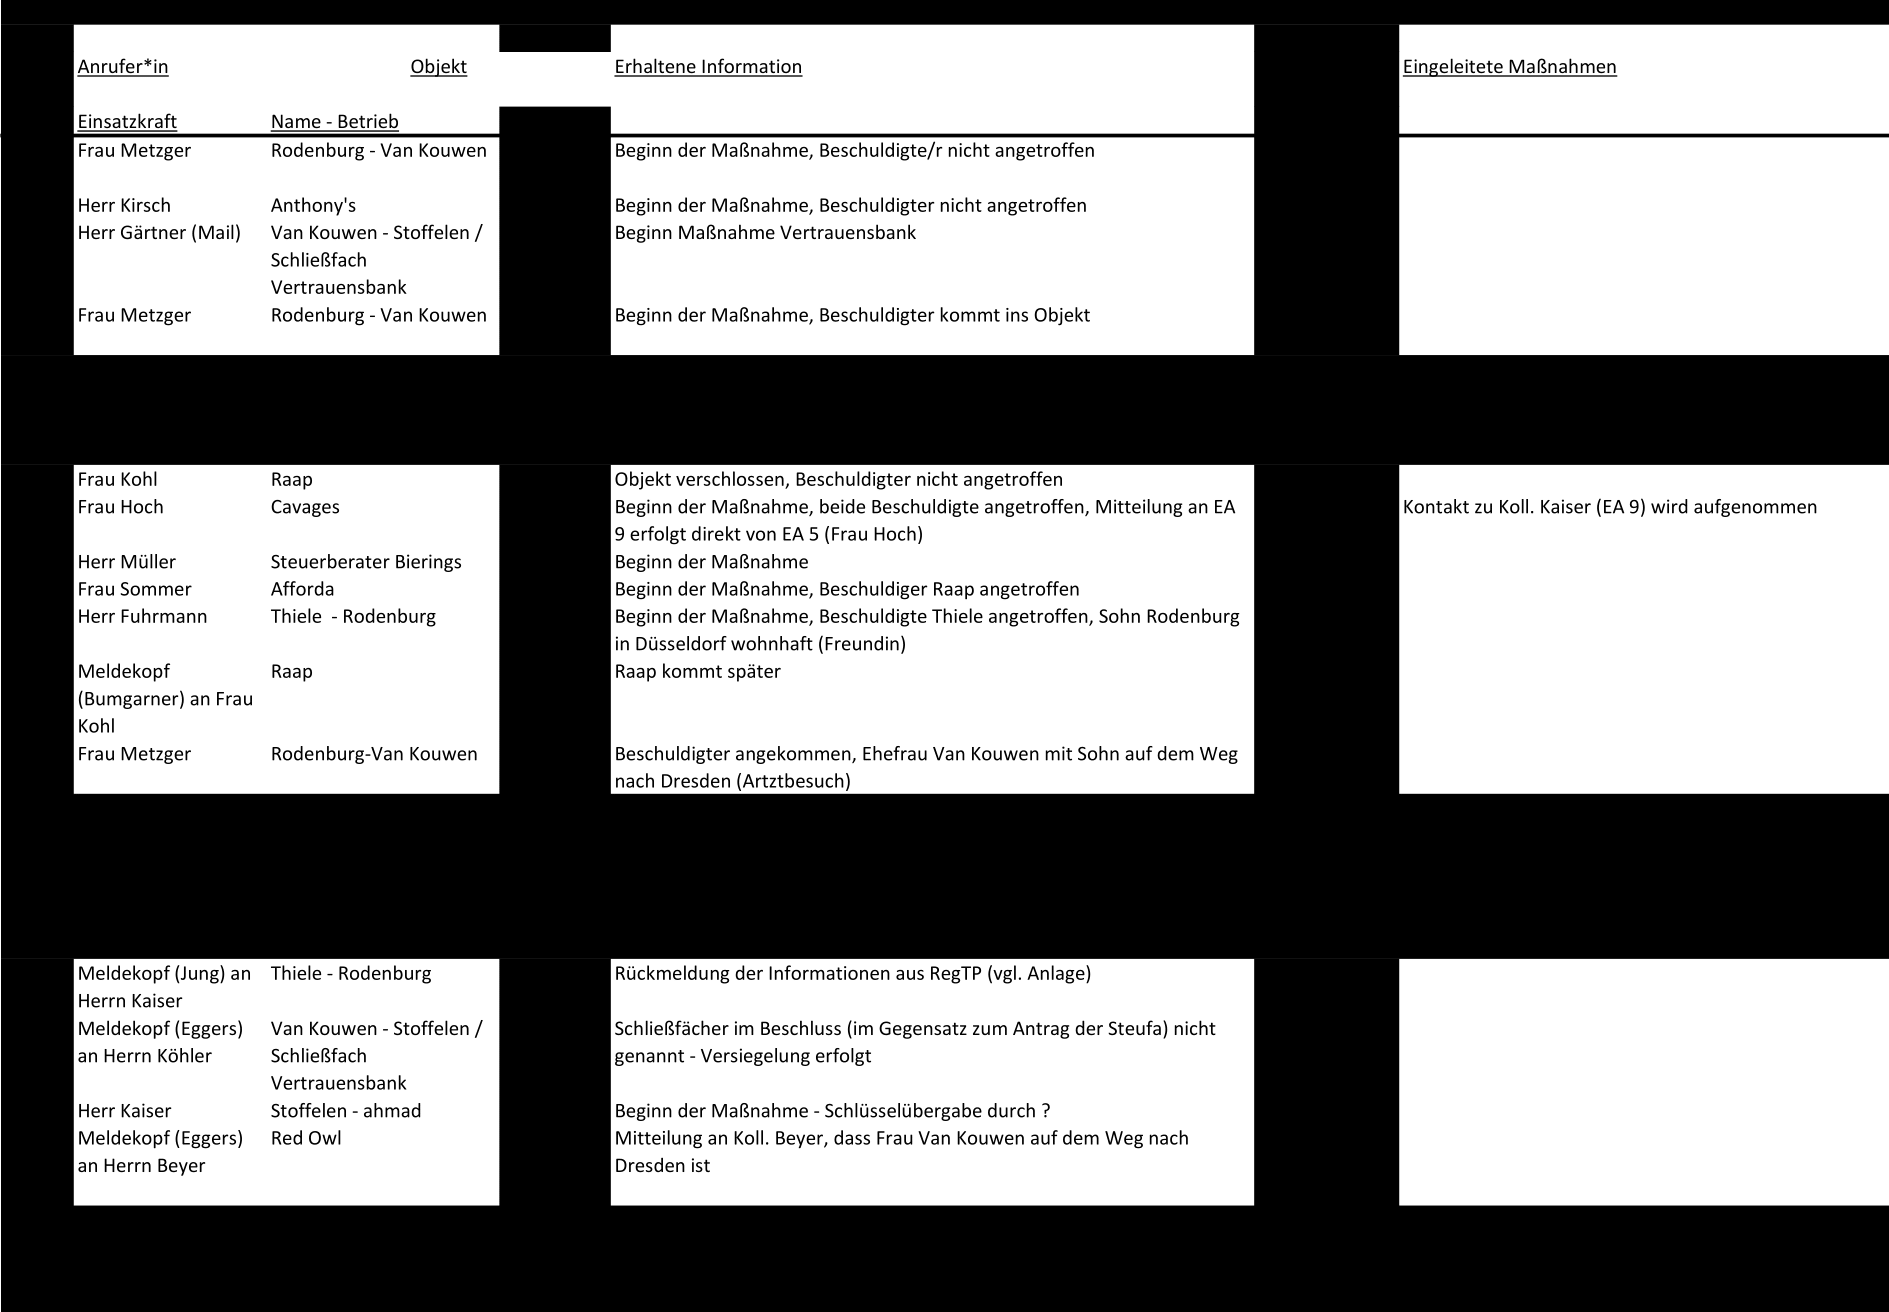
\includegraphics[width=.75\textwidth]{images/0-Artefaktmodell/Chronologie_Meldekopf-1.png}
    \caption{Artefaktmodell Meldekopf (1)}
    \label{fig:chrono1}
\end{figure}

Aus diesem lässt sich erkennen, welche Informationen über Beschuldigte und Objekte im Laufe der Durchsuchung benötigt werden.
Dadurch kann sichergestellt werden, dass das resultierende Produkt nur über die nötigen Funktionen verfügt und keine unhilfreichen Informationen direkt anzeigt.

\begin{figure}[htp]
    \centering
    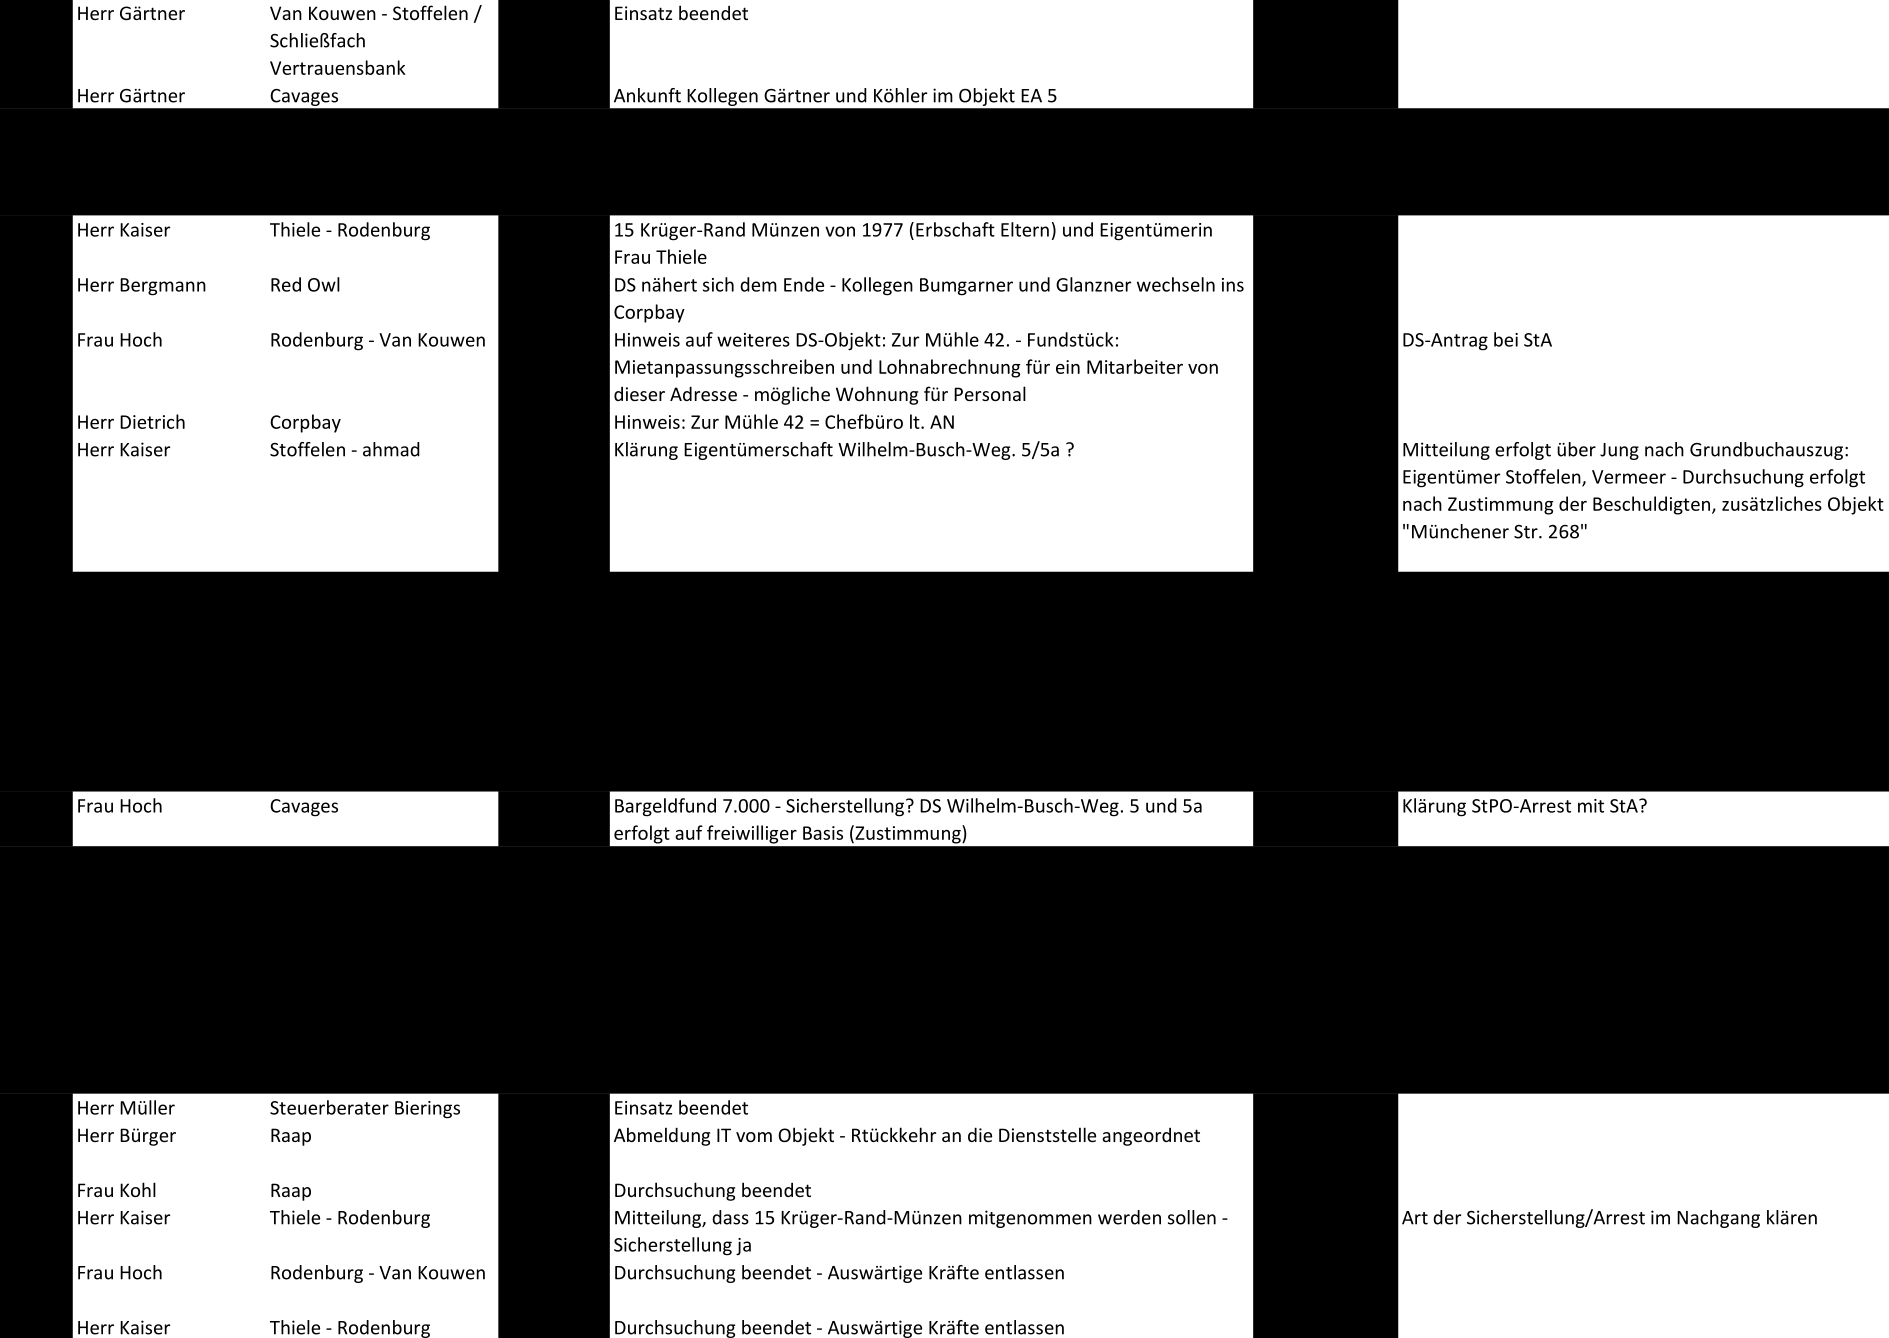
\includegraphics[width=.75\textwidth]{images/0-Artefaktmodell/Chronologie_Meldekopf-2.png}
    \caption{Artefaktmodell Meldekopf (2)}
    \label{fig:chrono2}
\end{figure}

Genauer beschrieben liegt bei dem Modell eine tabellarische Auflistung von Ereignissen der Durchsuchung vor.
Dabei verfügt die Tabelle über die Spalten "AnruferIn", "Objekt", "Erhaltene Informationen" und die optionale Spalte "Eingeleitete Maßnahmen".

Ein zentrale Funktion welche nach der Sichtung des Modells als nötig befunden wurde, im Interview im Kontext jedoch nicht zur Sprache kam ist das spontane Hinzufügen eines neuen Objekts während einer laufenden Durchsuchung.
Enthielte das Produkt diese Funktion nicht, so wäre es im Falle des Auftretens eines neuen Objekts nötig, dieses über die alte, papiergebunde Vorgehensweise zu koordinieren.
Ebenso kann festgestellt werden, dass das Modell nicht über konsistente Syntax innerhalb der Spalten verfügt. 
Am Anfang der zweiten Spalte ist die Überschrift "Name - Betrieb" zu lesen.
Diese Syntax wird zunächst eingehalten, später jedoch verworfen.
Erfahrungsberichte aus dem Interview im Kontext lassen darauf hindeuten, dass dies aus Zeitgründen geschah.

\begin{figure}[htp]
    \centering
    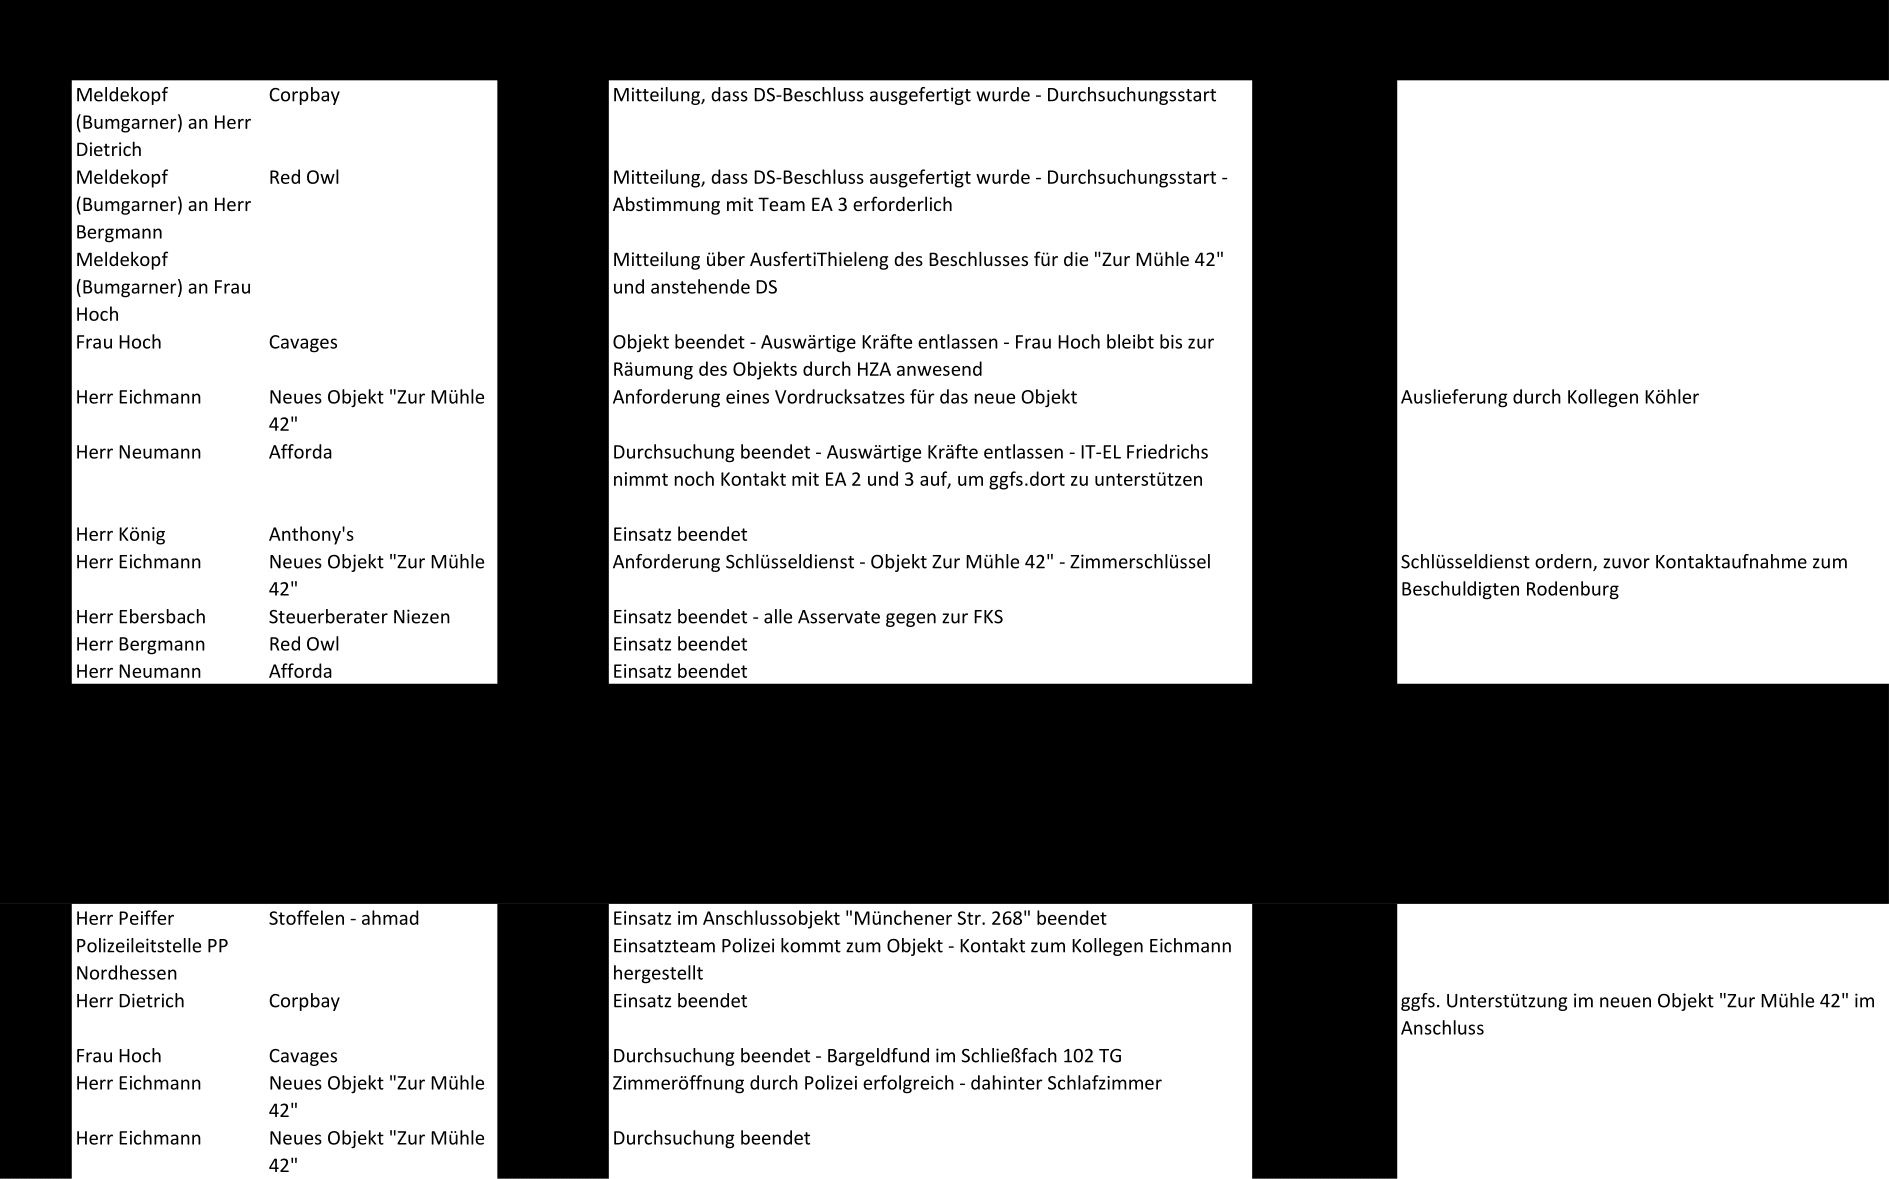
\includegraphics[width=.75\textwidth]{images/0-Artefaktmodell/Chronologie_Meldekopf-3.png}
    \caption{Artefaktmodell Meldekopf (3)}
    \label{fig:chrono3}
\end{figure}

Aus Gründen der Diskretion ist das Artefaktmodell in dieser Abgabe des Dokuments geschwärzt.
Des Weiteren wurden sämtliche Namen geändert und das Dokument gekürzt.
Dies bezieht sich sowohl auf Personen, Betriebe, als auch Straßennamen.
Im Zuge des nutzungsorientieren Prozesses lagen dem Autor jedoch Originaldokumente vor.

        \section{Persona} 

In diesem Abschnitt wird die im Zuge dieser Ausarbeitung entwickelte Persona vorgestellt.
Bei einer realen Umsetzung der NOG werden mehrerer Personas erstellt, damit ein möglichst breites Spektrum der Nutzenden in diesen abgebildet wird.
Die Persona dient im Folgenden auch als Handelnder im unter \autoref{sec:istSzenario} aufgeführten IST-Szenario.

\autoref{fig:personaPaul} zeigt eine grafische Beschreibung der Persona Paul Theiss, welche im Folgenden als fiktiver Repräsentant eines Steuerfahnders auftritt.
Paul ist 45 Jahre alt, verheiratet und hat zwei Kinder.
Er arbeitet seit Berufseintritt in der hessischen Finanzverwaltung.
In seiner Freizeit verbringt Paul gerne Zeit mit seiner Familie.
Wichtig anzumerken ist, dass Paul als fiktive Person die Entwicklung des momentan verwendeten Meldekopfsystems zugeschrieben wird. 
Weitere Informationen zur Persona Paul Theiss sind wie erwähnt \autoref{fig:personaPaul} zu entnehmen

Die im Folgenden zu findenden Handlungen und Personen sind erfunden. Ähnlichkeiten mit lebenden oder toten Personen sowie Handlungen sind rein zufällig. 

\begin{figure}
    \centering
    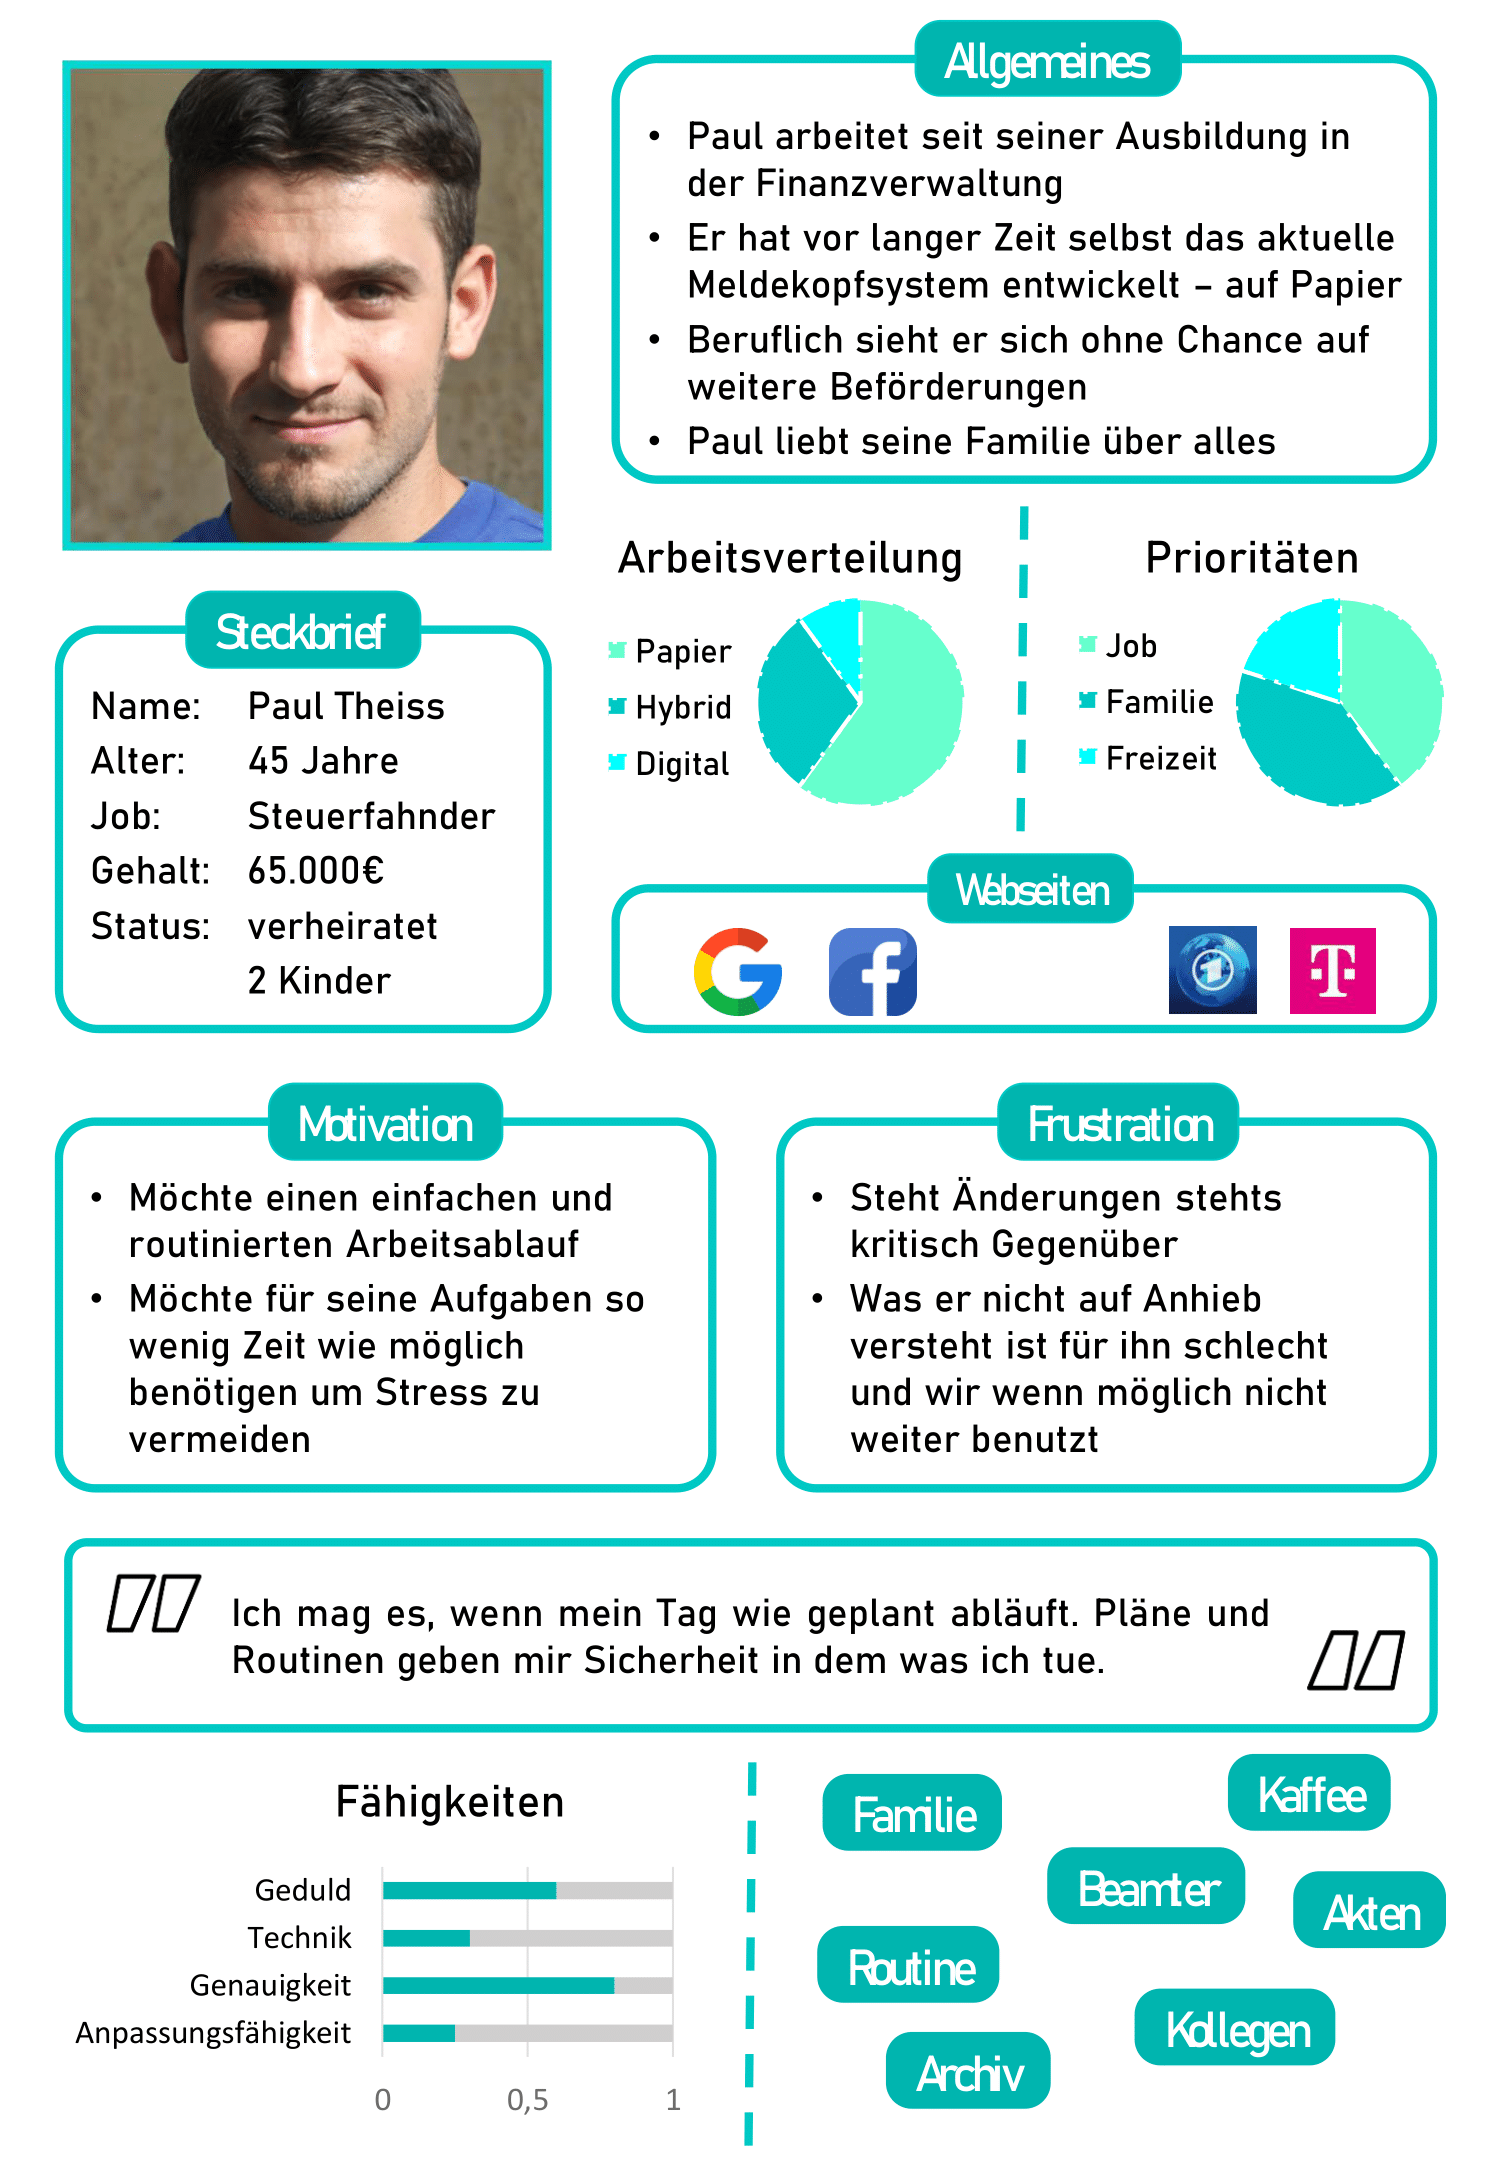
\includegraphics[width=\textwidth]{images/persona_1.png}
    \caption{Persona Paul Theiss}
    \label{fig:personaPaul}
\end{figure}
        \section{IST-Szenario}\label{sec:istSzenario}

Aus den im Interview im Kontext, sowie dem Artefaktmodell gewonnen Informationen über die Tätigkeiten des Meldekopfes wird nun ein beispielhaftes Szenario erstellt.
Im realen Prozess der nutzungsorientierten Gestaltung werden viele Szenarien erstellt, welche den vollen Kontext abdecken.
Dies ist nötig, damit im Laufe der Entwicklung alle Arbeitsschritte und Tätigkeiten bedacht werden können.
Aus Gründen des Umfangs dieser Arbeit wird jedoch auf weitere Szenarien verzichtet.

Das folgende Szenario "Mehr Personal wird angefragt" beinhaltet die Persona Paul Theiss, welche in diesem Moment im Meldekopf tätig ist.
Genauer geht es um den Prozess einer Anforderung von mehr Personal zu einem Objekt.

\subsection{IST-Szenario: Mehr Personal wird angefragt}

Paul ist momentan als Meldekopf für eine Durchsuchung eingeteilt. 
Er sitzt zusammen mit zwei Kollegen, Frau Beister und Herrn Diebold, in einem Besprechungsraum an einem großen tafelähnlichen Tisch. 
Jedes von der Durchsuchung betroffenes Objekt wird durch ein DIN A4 Blatt auf dem Tisch vor ihm repräsentiert. 
Auf diesen kann Paul ein Bild des Objekts, alle diesem momentan zugeordneten Kollegen und einige Bemerkungen erkennen. 
Die Informationen sind sehr klein gedruckt. 
Paul muss also um den Tisch laufen, um alle Objekte betrachten zu können. 
An seinem Sitzplatz steht ein Telefon, sowie Stifte und Haftnotizen. 
Momentan sitzt Paul an seinem Platz und wartet auf eine Aufgabe.

Pauls Telefon klingelt. 
Auf der anderen Seite ist Frau Schnee.
Paul erinnert sich, dass Frau Schnee momentan an Objekt D zugange ist, also steht er auf und stellt sich vor die Informationen zu diesem Objekt. 
Aus dem Augenwinkel sieht er, dass Frau Schnee Objektleiterin von Objekt D ist. 
Diese erklärt Paul indessen, dass ihr Team einen vorher nicht bekannten Keller unter dem Objekt gefunden hat, welcher ebenfalls durchsucht werden muss. 
Dazu möchte sie mehr Personal anfordern. Paul entgegnet, dass er sich bemüht Personal zu finden und zurückrufen wird, sobald es Neues gibt.

Sobald Paul aufgelegt hat, fragt er zunächst seine beiden Kollegen nach momentan freien Kollegen, welche er zu Frau Schnee schicken kann. 
Diese verneinen die Nachfrage jedoch. Paul überfliegt nun alle Objektzettel. 
Genauer schaut er, ob unter „Bemerkungen“ vermerkt wurde, dass an einem Objekt entbehrliches Personal abgezogen werden kann. 
Leider ist dies nirgends der Fall. 
Paul nimmt sich also einen Stift und vermerkt sein neues Wissen zu Objekt D in dessen Bemerkungen. 
Ebenso merkt er dort an, dass mehr Personal nötig ist. 
Daraufhin ruft er Frau Schnee zurück, um ihr die schlechten Neuigkeiten mitzuteilen. 
Er will sie jedoch informieren, sobald Kollegen frei werden.

[Es vergeht etwas Zeit]

Wieder klingelt Pauls Telefon. 
Dieses Mal ist Herr Sebert, Objektleiter von Objekt B auf der anderen Seite. 
Dieser informiert Paul, dass die Maßnahmen an seinem Objekt abgeschlossen sind. 
Paul bedankt sich für die Information und möchte Herrn Siebert samt seinen Kollegen schon zurück in die Dienststelle schicken als ihm einfällt, dass Frau Schnee noch immer auf Unterstützung wartet. 
Dies teilt Paul Herrn Sebert mit. 
Er läuft zu den Informationen zu Objekt D, um Herrn Sebert die Adresse des neuen Objekts mitzuteilen. 
Dieser verabschiedet sich und macht sich mit seinen Kollegen auf den Weg zu Frau Schnee.
Paul macht einen großen Hacken an den Zettel zu Objekt B um dieses für alle im Raum als abgeschlossen zu kennzeichnen. 
Daraufhin nimmt der die Papierstreifen der diesem Objekt zugeordneten Kollegen und legt diese zu Objekt D. 
In dessen Bemerkungen notiert er die Verschiebung der Kollegen samt aktueller Zeit. 
Zuletzt ruft er erneut bei Frau Schnee an, um diese über die kommenden Kollegen zu informieren. 
Frau Schnee bedankt sich und geht daraufhin zurück an ihre Arbeit.

Wenig später ruft erneut Herr Sebert an. 
Er teilt Paul mit, dass sein Team am neuen Einsatzort angekommen ist und sich ab jetzt in das Team von Frau Schnee eingliedert. 
Damit ist für Paul die Aufgabe erledigt. 
Dies kennzeichnet er mit einem Hacken hinter dem vermerkten Wunsch auf Unterstützung in den Bemerkungen von Objekt D.


    \chapter{Gestaltung SOLL-Zustand}\label{sec:gestaltung}

Nach der Erfassung des IST-Zustandes erfolgt nach dem Prozess der NOG nun die Definition eines SOLL-Zustandes.
Dieser wird auf den ermittelten Informationen über den IST-Zustand, sowie den Aspekten und Kriterien nutzungsorientierter Gestaltung aufbauen.

Zunächst wird hierzu das bereits erstellte IST-Szenario in ein SOLL-Szenario umgewandelt.
Dabei bleiben Aufgabe und Kontext erhalten, die Handelnden verfügen nun jedoch über optimierte technische Hilfe.
Aus diesem SOLL-Szenario wird sodann ein Prototyp erstellt und vorgestellt.

In der Realität verfüge dieser Abschnitt über mehrere SOLL-Szenarien und einen umfangreicheren Prototyp.
Auf Grund der Kompaktheit der Veranstaltung und dem Umfang dieses Dokuments wird jedoch auf zusätzliche Szenarien verzichtet.
Ebenso werden nur die für das gegebene Szenario wichtigen Ausschnitte des Prototyps gezeigt. 
        \section{SOLL-Szenario}\label{sec:sollSzenario}

Aus den aus dem IST-Zustand gewonnen Informationen über die Tätigkeiten des Meldekopfes wird nun mit Hilfe der nutzungsorientierten Aspekte ein beispielhaftes SOLL-Szenario erstellt.
Dieses basiert auf den Abläufen des IST-Szenarios in \autoref{sec:istSzenario}.

Im realen Prozess der nutzungsorientierten Gestaltung werden viele Szenarien erstellt, welche den vollen Kontext abdecken.
Dies ist nötig, damit im Laufe der Entwicklung alle Arbeitsschritte und Tätigkeiten bedacht werden können.
Aus Gründen des Umfangs dieser Arbeit wird jedoch auf weitere Szenarien verzichtet.

Das folgende Szenario "Mehr Personal wird angefragt" beinhaltet die Persona Paul Theiss, welche in diesem Moment im Meldekopf tätig ist.
Genauer geht es um den Prozess einer Anforderung von mehr Personal zu einem Objekt.
In diesem SOLL-Szenario steht ihm die nutzungsorientierte Software zur Verfügung.

\subsection{SOLL-Szenario: Mehr Personal wird angefragt}

Paul ist momentan als Meldekopf für eine Durchsuchung eingeteilt. 
Er sitzt zusammen mit zwei Kollegen, Frau Beister und Herrn Diebold, in einem Besprechungsraum an einem großen tafelähnlichen Tisch. 
Im Raum steht ein Smart-Board, auf welchem der Übersichtsscreen der DCC geöffnet ist. 
Dieser enthält alle wichtigen Informationen zu allen an der Durchsuchung beteiligten Objekten. 
Die Ansicht kann auf Wunsch nach vielen Kriterien gefiltert werden. 
Momentan sitz Paul an seinem Platz und wartet auf eine Aufgabe. 
Vor sich hat Paul einen Laptop mit der Eingabemaske des DCC.

Pauls Telefon klingelt. 
Auf der anderen Seite ist Frau Schnee. 
Auf dem DCC sieht Paul, dass Frau Schnee momentan an Objekt D als Objektleiterin zugange ist. 
Frau Schnee erklärt Paul, dass ihr Team einen vorher nicht bekannten Keller unter dem Objekt gefunden hat, welcher ebenfalls durchsucht werden muss. 
Dazu möchte sie mehr Personal anfordern. 
Paul sieht direkt am DCC, dass momentan kein freies Personal verfügbar ist. 
Er entgegnet Frau Schnee, dass er sich melden wird, sobald er freies Personal für ihr Objekt findet. 

Über die Eingabemaske gibt Paul an, dass Objekt D Verstärkung benötigt. 
Dabei referenziert er das Objekt direkt und stellt die Dringlichkeit auf „wichtiges ToDo“. 
Ebenso notiert er den Fund des Kellers unter dem Objekt über die Eingabemaske, damit dies im Endprotokoll erscheint.

[Es vergeht etwas Zeit]

Wieder klingelt Pauls Telefon. 
Dieses Mal ist Herr Sebert, Objektleiter von Objekt B auf der anderen Seite. 
Dieser informiert Paul, dass die Maßnahmen an seinem Objekt abgeschlossen sind. 
Paul sieht auf dem Übersichtsscreen, dass Frau Schnee noch immer Personal an Objekt D benötigt. 
Mit einem Klick auf dieses sieht Paul die Adresse des Objekts, welche er Herrn Sebert mitteilt, damit er sich mit seinem Team auf den Weg machen kann. 
Dieser verabschiedet sich und macht sich mit seinen Kollegen auf den Weg zu Frau Schnee.

Paul nutzt nun den vorbereiteten Vorgang „verschieben“ in der Eingabemaske um das Team von Herrn Sebert zu Objekt D zu verschieben. 
Ebenso gibt er an, dass die Durchsuchung von Objekt B abgeschlossen ist. 
Dieses verschwindet aus der Übersicht. Zuletzt ruft Paul erneut bei Frau Schnee an, um diese über die kommenden Kollegen zu informieren. 
Frau Schnee bedankt sich und geht daraufhin zurück an ihre Arbeit.

Wenig später ruft erneut Herr Sebert an. 
Er teilt Paul mit, dass sein Team am neuen Einsatzort angekommen ist und sich ab jetzt in das Team von Frau Schnee eingliedert. 
Paul wählt in der Eingabemaske unter „Aktionen abschließen“ das Eintreffen des Teams an Objekt D aus, um die Ankunft auch für das Protokoll zu dokumentieren.
Damit ist für Paul die Aufgabe erledigt. 

        \section{Prototyp}\label{sec:prototypPraktisch}

Bevor die Erstellung von Prototypen für den Nutzungskontext beginnen konnte, müssen einige Überlegungen angestellt werden.
Im Gegensatz zu einigen anderen Kontexten muss hier Software von Grund auf entwickelt werden.
Hierzu wird zunächst überlegt, wie eine auf \autoref{sec:sollSzenario} aufbauende Software beschaffen sein muss.
Im zweiten Schritt werden konkrete designspezifische Überlegungen angestellt. 
Diese werden anhand einiger Mockups vorgestellt.

\subsection{Vorüberlegungen}

Aus dem in \autoref{sec:sollSzenario} zu findenden Soll-Szenario ist abzuleiten, dass die Software über mindestens zwei Hauptansichten verfügen muss.
Dabei eignet sich eine dieser Ansichten (ab hier Übersicht genannt) zur Darstellung der an der Durchsuchung beteiligten Personen und Objekten.
Diese soll vorzugsweise auf einem interaktiven Touch Display (beispielsweise der Firma SmartBoard) betrieben werden, damit alle sich im Raum befindlichen Personen eine möglichst gute Einsicht auf diese Übersicht haben.
Die Übersicht soll neben den Personen und Objekten ebenfalls alle eingegebenen Informationen darstellen.
Dies soll anhand einer Timeline geschehen, welche sich an dem Design einer Twitter Timeline\footnote{\url{https://twitter.com/TwitterSupport/status/1501989523588358145}} orientiert.
Des Weiteren soll diese Ansicht über eine Filter Funktion für Objekte verfügen, welche des den Nutzenden erlaubt, schnell und einfach Zugang zu den gewünschten Informationen zu erhalten.

Bei der zweiten Ansicht handelt es sich um eine Eingabemaske.
Diese wird simultan in mehreren Instanzen auf Notebooks ausgeführt.
Ziel ist es hier, jeder sich im Meldekopf befindlichen Person eine möglichst bequeme Möglichkeit zu geben, zu jeder Zeit neue Informationen zu erfassen.
Um diese Produktivität des Systems zu maximieren, soll die Eingabemaske über einige Hilfen verfügen.
Es soll möglich sein, mit Hilfe einer automatischen Vervollständigung schnell Personen oder Objekte zu referenzieren.
Ebenso sollen oft verwendete Informationen in Form von Templates gespeichert sein, welche auf Wunsch nur mit den betreffenden Personen und Objekten gefüllt werden müssen.
Damit stets eine Übersicht über alle Vorgänge der Durchsuchung herrscht, soll auch hier die bereits erwähnte Timeline für Informationen eingefügt werden.

Im Idealfall wird das neue System also von mehreren Bildschirmen und Eingabegeräten zur selben Zeit betrieben. 
Bei der Erstellung von Mockups soll darauf geachtet werden, welche Eingabegeräte an den zu den Ansichten vorgesehenen Geräten zur Verfügung stehen.

\subsection{Mockups}

Aus dem soeben festgelegten Konzept werden nun Mockups erstellt.
Wird im Gegensatz zu Mockups nicht rein auf die Anordnung von Elementen, sondern auch auf deren Darstellung geachtet.
Die Mockups sind in zwei Kategorien eingeteilt. 
Zuerst zu sehen sind Mockups, welche das Design der Eingabemaske wiedergeben.
Auf diese folgen Mockups zum Übersichtsbildschirm.
Aus Gründen des Umfangs umfasst dieses Dokument nicht alle erstellten Mockups.
Der Inhalt dieser wird jedoch durch textuelle Beschreibungen ersetzt.

\subsubsection{Eingabemaske}

Die Mockups der Eingabemaske spiegeln das Verschieben einer Person zu einem neuen Objekt wider.
\autoref{fig:inputStart} zeigt hierbei den initialen Zustand der Eingabemaske.
Im oberen Bereich finden sich Möglichkeiten Personen und Objekte zu referenzieren, daneben die Funktion zum Laden eines Templates, hier "Vorbereitete Vorgänge" genannt.
In diesem Mockup sind nur zwei Templates zu sehen.
Mehr Templates sollen über die Zeit hinzugefügt werden.
Hierzu muss das Programm des Öfteren Bei Großdurchsuchungen zum Einsatz kommen.
Hierbei werden fehlende Templates schnell ausfindig gemacht.

\begin{figure}[htp]
    \centering
    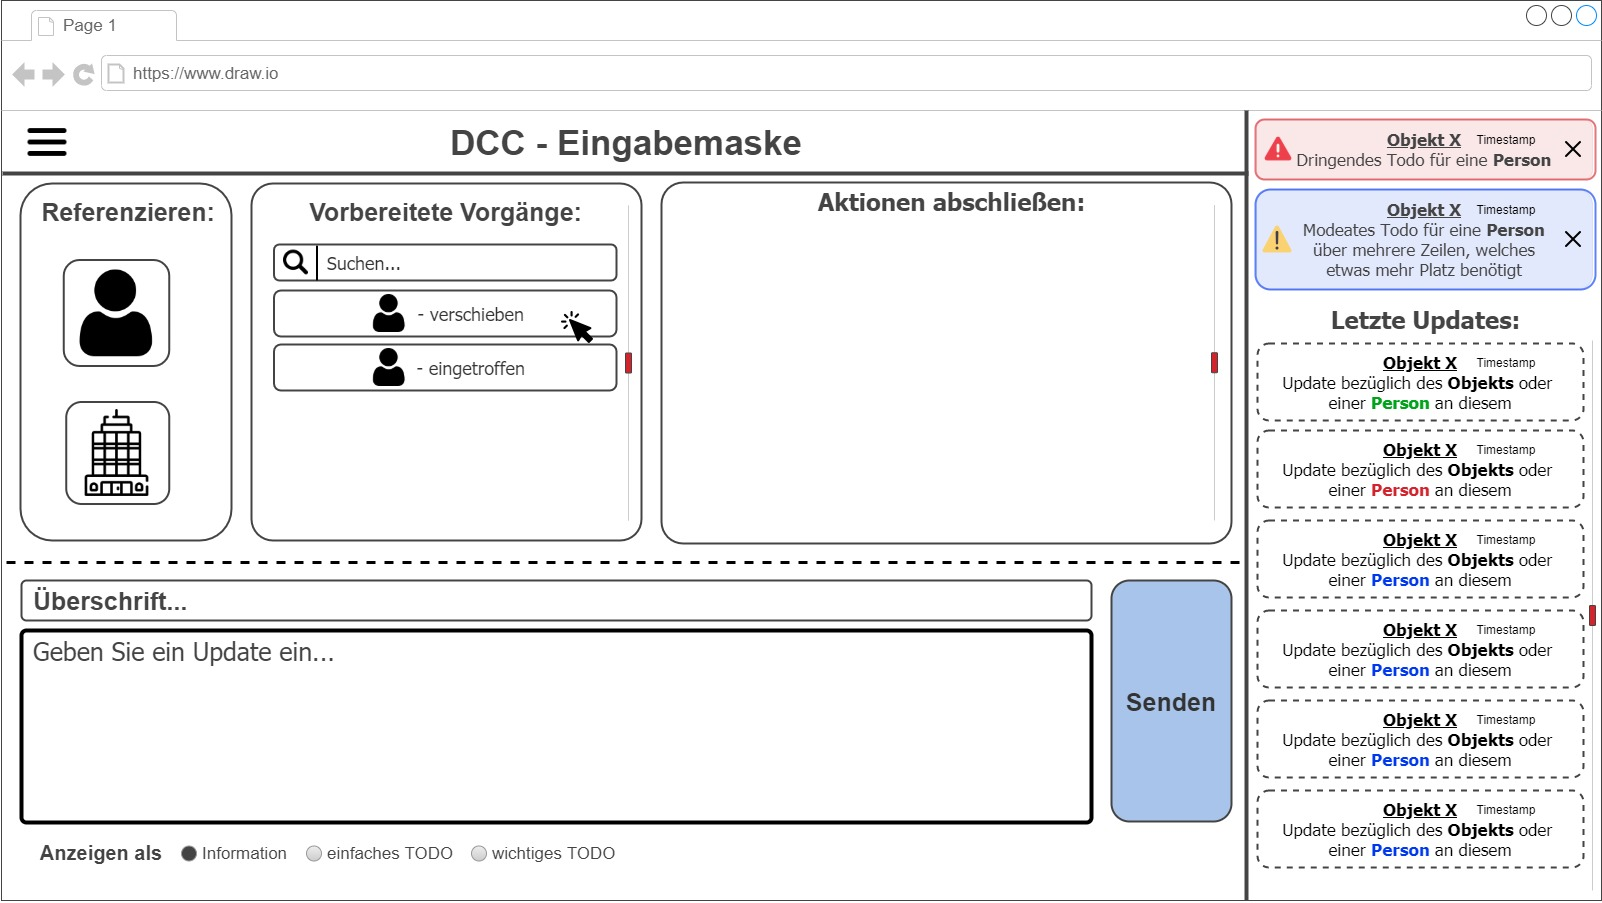
\includegraphics[width=\textwidth]{images/1-MockupsV1/InputScreenStart.jpg}
    \caption{Eingabemaske Start}
    \label{fig:inputStart}
\end{figure}

Rechts neben den Templates findet sich ein Bereich zum Abschließen von Aktionen.
Beispielsweise erscheint dort das bereits ausgefüllte Template "Personen eingetroffen", wenn diese zuvor verschoben wurden.
Unter diesen drei Boxen findet sich die eigentliche Eingabemöglichkeit.
Nutzende geben hier Überschrift und Nachricht ein, bevor sie diese über den Button absenden können.
Unter diesen Eingabefeldern findet sich eine Auswahl für die Darstellung der Updates.
Hier kann zwischen einer normalen Darstellung und zwei angepinnten Varianten entschieden werden.

Diese Wahl wirkt sich direkt auf die rechts dargestellte Timeline aus.
Erkenntlich ist, dass diese über drei Darstellungsarten verfügt.
Weiß steht hier für eine einfache Information, welche keine weiteren Aktionen benötigt.
Blau und Rot stehen für angepinnte Informationen oder auch ToDos. 
Diese werden stets am oberen Ende der Timeline angezeigt.
Über das Kreuz kann ein ToDo als erledigt erklärt werden.
Erledigte ToDos werden in normale Informationen umgewandelt und normal in der Timeline angezeigt.

\begin{figure}[htp]
    \centering
    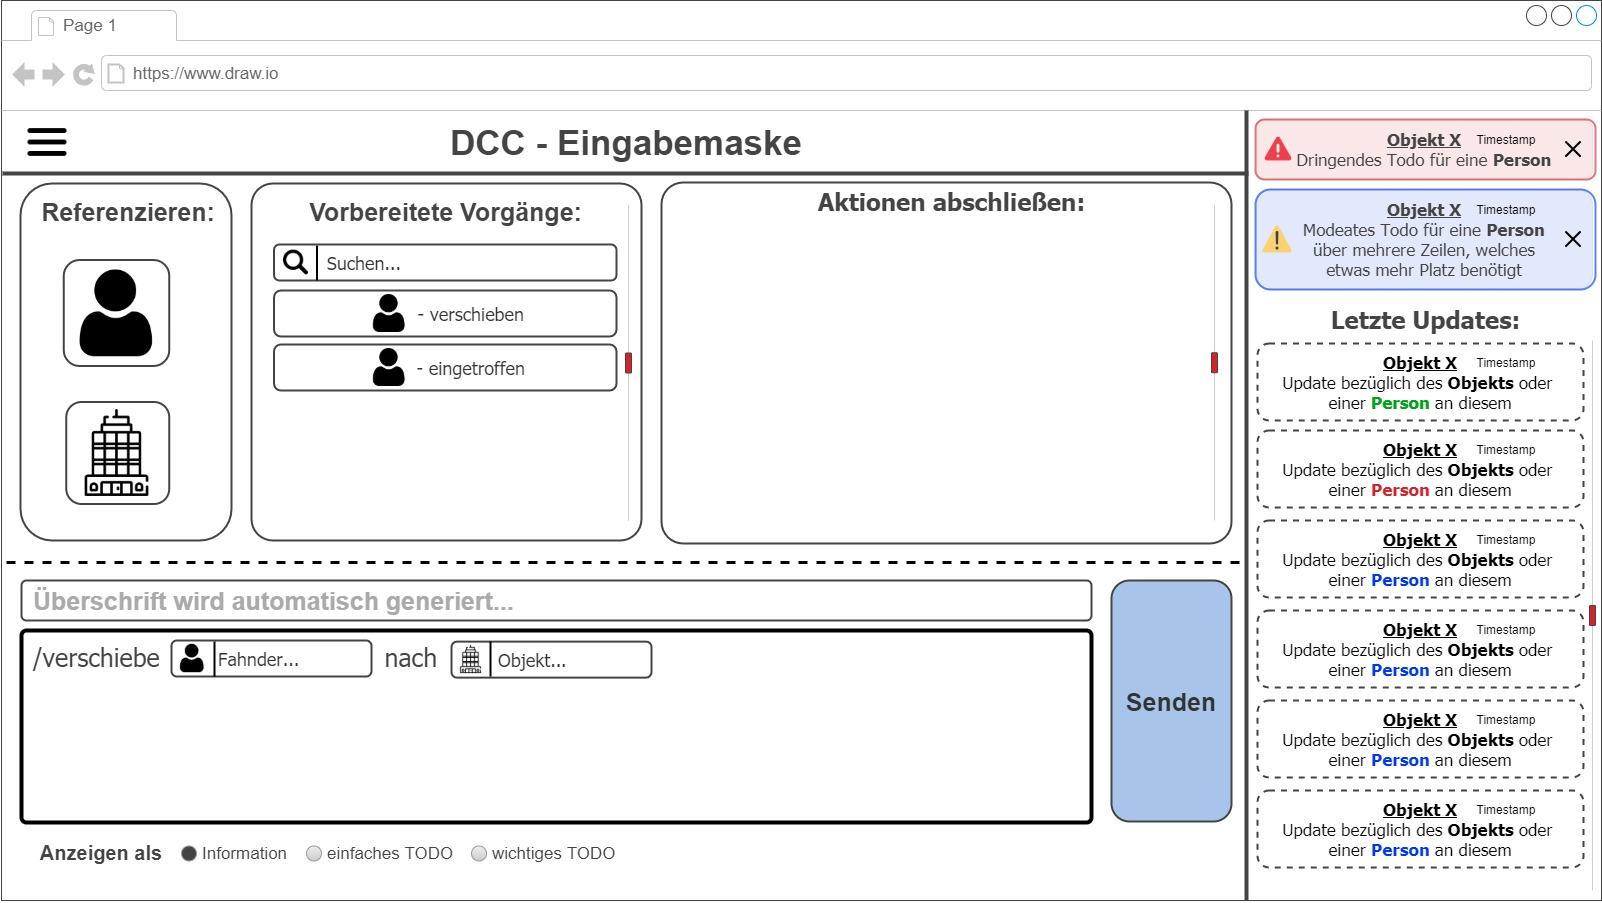
\includegraphics[width=\textwidth]{images/1-MockupsV1/InputScreenMiddle.jpg}
    \caption{Eingabemaske im Vorgang}
    \label{fig:inputMiddle}
\end{figure}

Wie bereits angemerkt stellen diese Mockups den Prozess des Verschiebens einer Person nach.
Hierzu wird nun im in \autoref{fig:inputStart} zu sehenden Mockup auf die Schaltfläche "Person verschieben" geklickt.
Wie erwartet lädt das Programm sodann das ausgewählte Template in die Eingabe.
Das Resultat dessen ist in \autoref{fig:inputMiddle} zu erkennen.

Das Eingabefeld der Überschrift ist nun deaktiviert, da im Fall der Verschiebung von Personen eine automatisch generierte Überschrift verwendet werden soll.
Darunter ist das Template "Person verschieben" zu sehen.
Das dem Text vorangestellt Slash Zeichen indiziert hierbei dem System, dass es sich über eine normale Nachricht hinaus um einen Befehl zum Ändern des Datenmodells handelt.
Neben des Slash Zeichens wurde ein von den Nutzenden auszufüllender Lückentext generiert.
Dieser enthält einen Satz, welcher den ausgewählten Vorgang beschreibt, in diesem Fall "Verschiebe [Person] nach [Objekt]".
Die Lücken können hierbei ausgefüllt werden, indem mit der Maus in sie geklickt wird.

Sollen mehrere Personen verschoben werden, so können mehr Personenfelder generiert werden, indem entweder unter "Referenzieren" auf die Person geklickt wird oder das Zeichen "@" eingefügt wird.
Nach dem Abschicken erkennt das Programm, dass mehrere Personen verschoben wurden und führt die Änderung im Datenmodell dementsprechend aus.

Wurde nun in das Eingabefeld für eine Person geklickt, so öffnet sich ein wie in \autoref{fig:inputEnd} dargestelltes Auswahlfenster, welches die verfügbaren Personen in alphabetischer Reihenfolge anzeigt.
Wird eine Eingabe im Feld getätigt, so passt sich das Auswahlfenster insofern an, dass nur zur aktuellen Eingabe passende Personen angezeigt werden.
Eine Person kann ausgewählt werden, indem mit der Maus auf sie geklickt wird.
Ebenso wird die oberste Person beim Drücken der Tabulator Taste ausgewählt.


\begin{figure}[htp]
    \centering
    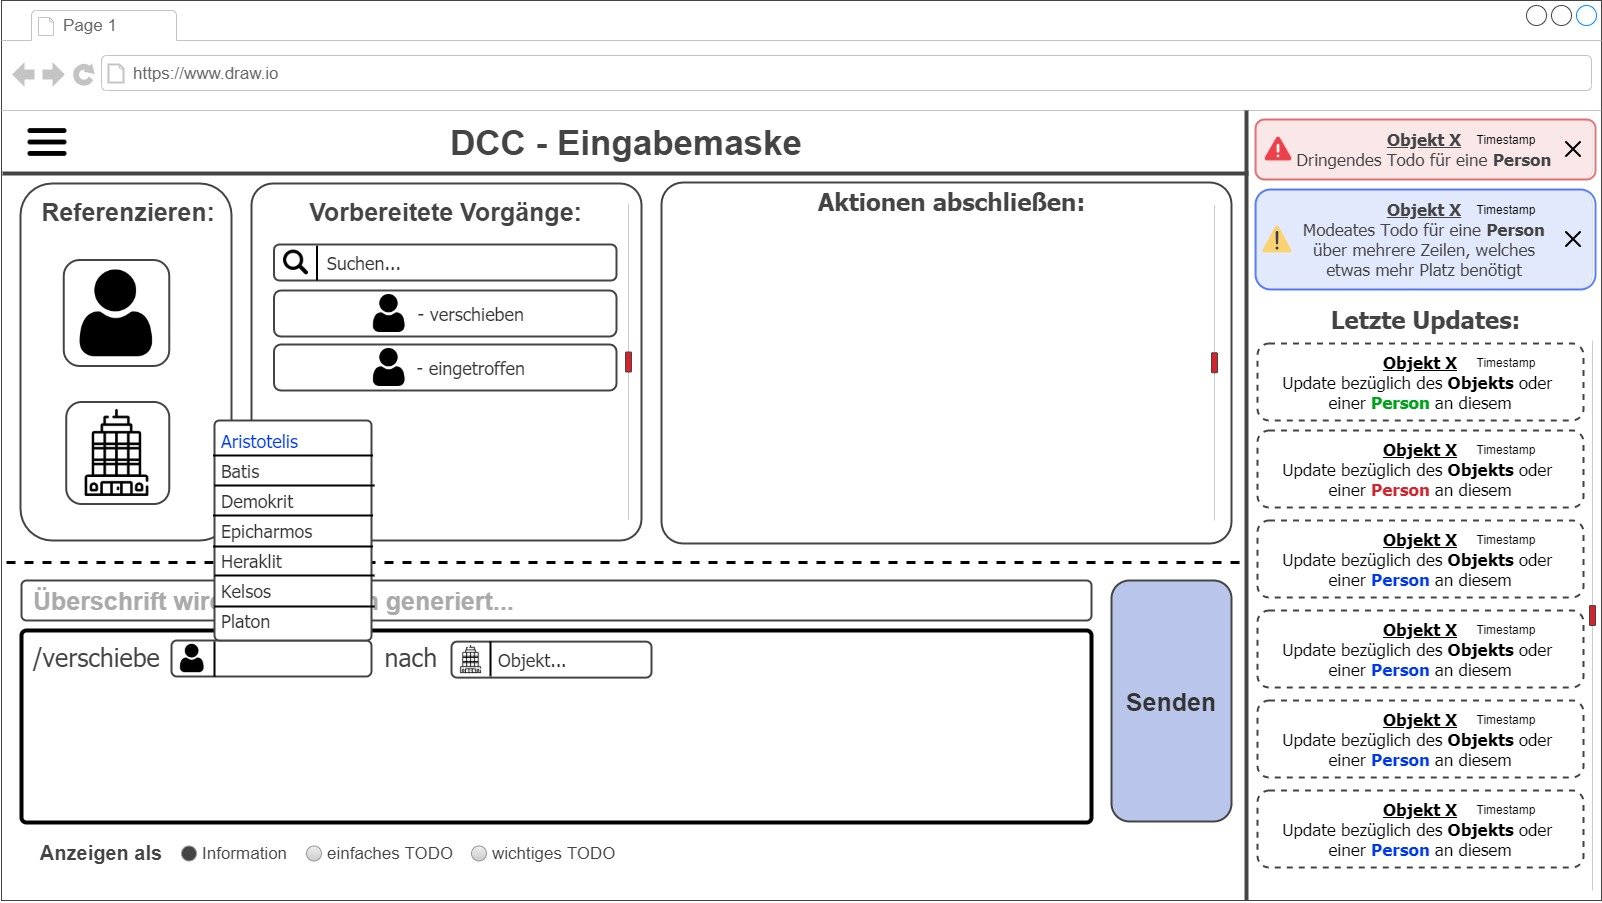
\includegraphics[width=\textwidth]{images/1-MockupsV1/InputScreenEnd.jpg}
    \caption{Eingabemaske Ende}
    \label{fig:inputEnd}
\end{figure}

Ist das Template vollständig ausgefüllt, kann es über die "Senden" Taste abgeschickt werden.
Dabei findet zunächst eine Konsistenzprüfung der angegebenen Daten statt.
Werden Fehler im Ausfüllprozess erkannt, so wird das Template nicht abgeschickt und den Nutzenden eine Fehlermeldung angezeigt.

Nach dem Abschicken des Templates werden die Eingabefelder geleert, sowie die Eingabe einer Überschrift wieder aktiviert.
In der Timeline erscheint ein neues Item, welches Titel und Inhalt des soeben abgeschickten Templates trägt.
Das Slash Zeichen wird dabei entfernt und Personen und Objektfelder durch Namen und Objektkennungen ersetzt.

Damit ist der Prozess des Verschiebens in der Eingabemaske abgeschlossen.
Es folgt eine Darstellung desselben Prozesses auf dem Übersichtsbildschirm.

\newpage
\subsubsection{Übersichtsbildschirm}

Nach abgeschlossenem Studieren des Konzepts der Eingabemaske wird nun ein Fokus auf den Übersichtsbildschirm gelegt.
\autoref{fig:viewStart} zeigt diesen vor der Durchführung des Verschiebens von Personen.
Dabei ist der linke Teil des Bildschirms der Kern des Übersichtsbildschirm.
Dieser besteht aus einem Bereich, welcher die Filterung der angezeigten Objekte umfasst, den Objekten selbst und einer Zeile, welche Personen anzeigt, welche sich an keinem Objekt befinden.

Seien zunächst die Funktionen des Filters aufgeführt.
Verschiedene Filter können über ein Dropdown Menü gewählt werden.
Dabei werden gewählte Filter rechts neben diesem Menü angezeigt.
Soll ein Filter abgewählt werden, so kann auf das Kreuz neben diesem Filter geklickt werden.
Es stehen einige voreingestellt Filter zur Verfügung.
Dabei handelt es sich beispielsweise um eine Auswahl des Objekttyps (Wohnung, Betrieb, ...) oder das Bundesland, in welchem sich das Objekt befindet.
Zusätzlich können Nutzende eigene Filter erstellen.
Dies funktioniert über ein System von Tags.
Jedem Objekt können beliebig viele Tags hinzugefügt werden, welche später als Filter gewählt werden können.

\begin{figure}[htp]
    \centering
    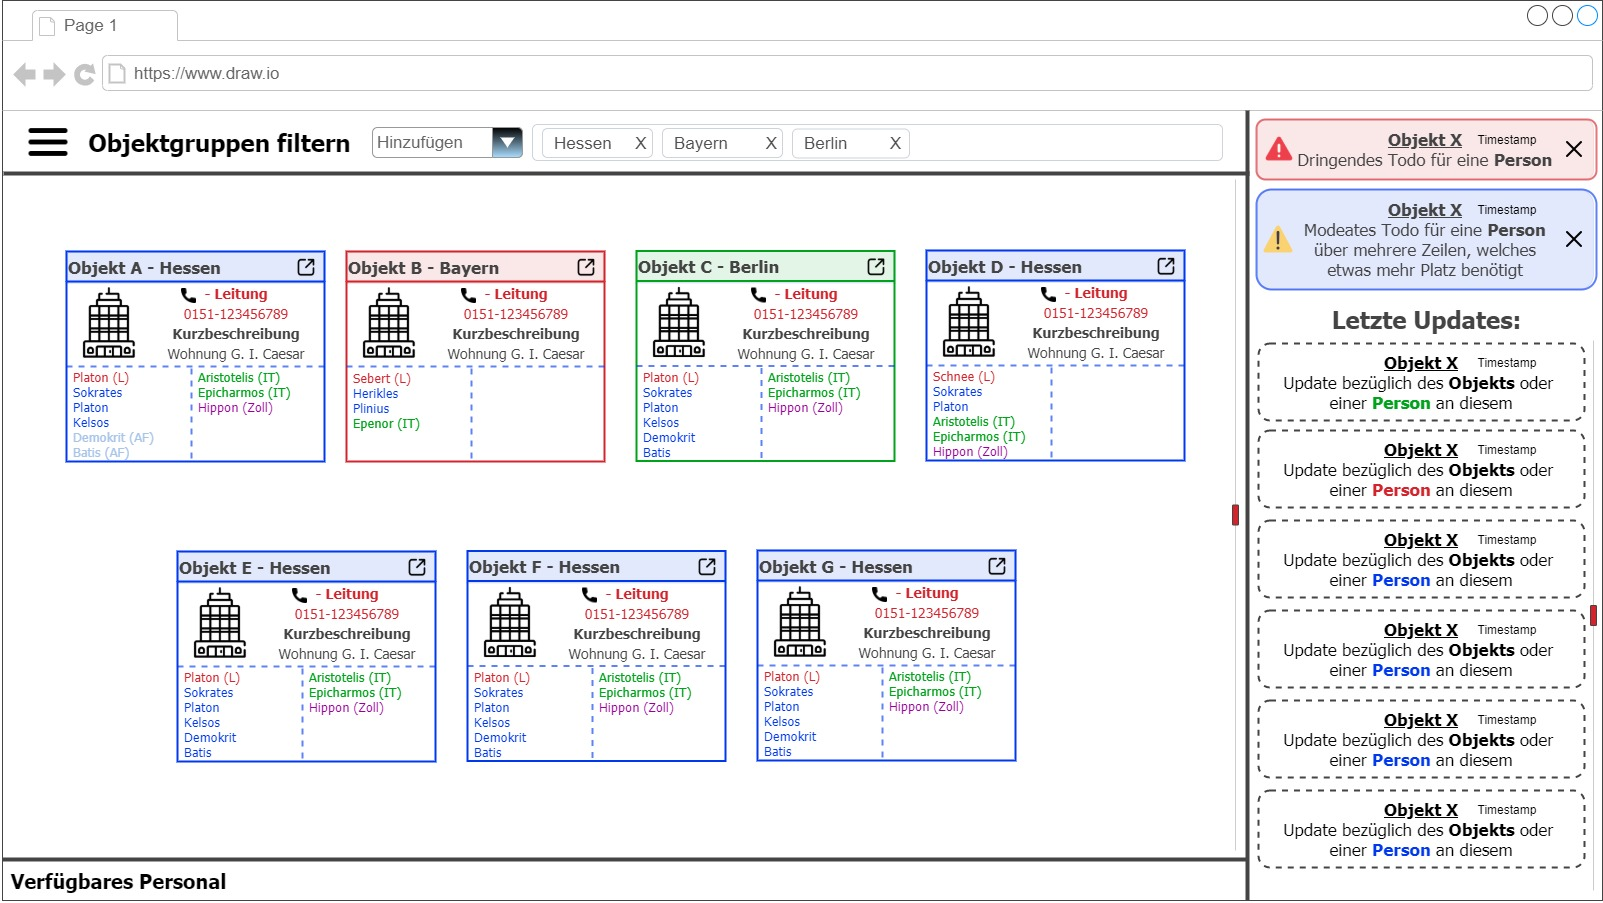
\includegraphics[width=\textwidth]{images/1-MockupsV1/ViewScreenLessBeforeMove.jpg}
    \caption{Übersichtsbildschirm Start}
    \label{fig:viewStart}
\end{figure}

Objekte werden als farbige Kästen dargestellt.
Dabei indiziert die Farbe das Bundesland des Objekts.
Zu jedem Objekt sind Kennung, Bundesland, Telefonnummer der Objektleitung, eine Kurzbeschreibung und das dort tätige Personal direkt ersichtlich.
Weitere Informationen zu einem Objekt können über den Button oben rechts angezeigt werden.
Dies wird durch ein Modalfenster realisiert.
Ebenso in der Überlegung befand sich hier ein an den Home-Bildschirm von Smartphones angelegtes System aus mehreren Ansichten, welche durch wischen geändert werden können.
Zu Gunsten des Überblicks fiel die Wahl jedoch auf das Modalfenster.
Personen sind ebenfalls eingefärbt.
Sie sind somit nach ihrem Einsatzgebiet gruppiert.

Unter den Objekten werden alle momentan verfügbaren Personen angezeigt.
Eine Person gilt als verfügbar, sobald sie keinem Objekt zugeordnet ist.
Neben einer Person wird hier ebenfalls ihr letzter Aufenthaltsort angezeigt.

\begin{figure}[htp]
    \centering
    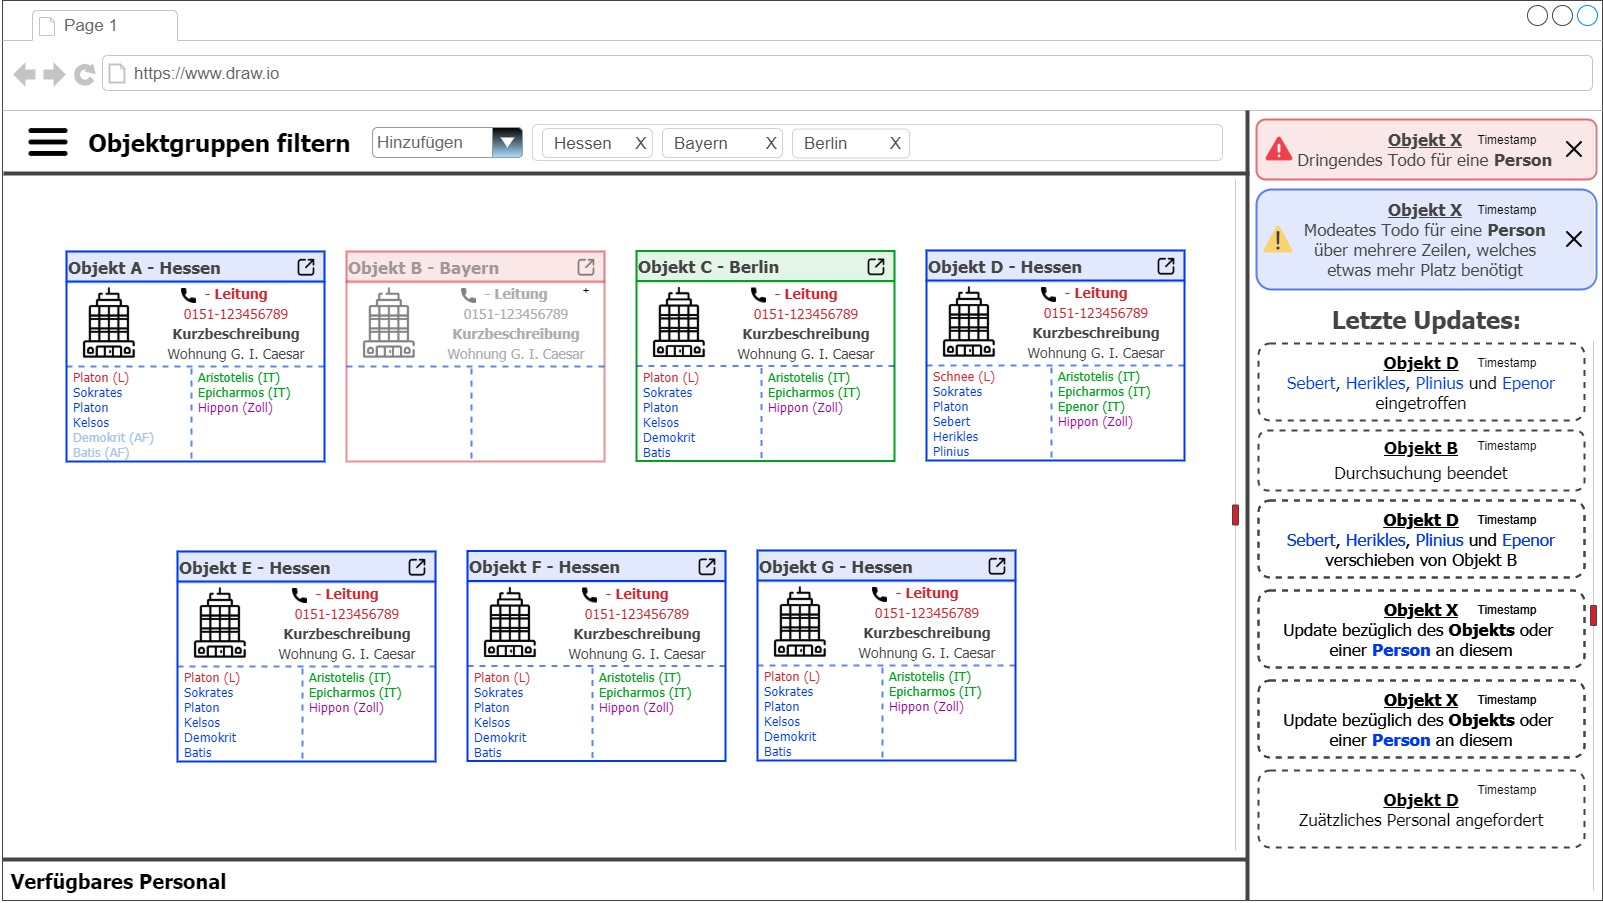
\includegraphics[width=\textwidth]{images/1-MockupsV1/ViewScreenLessAfterMove.jpg}
    \caption{Übersichtsbildschirm Ende}
    \label{fig:viewEnd}
\end{figure}

Es werden nun alle Personen von Objekt B nach Objekt D verschoben.
Darüber hinaus wird die Durchsuchung in Objekt B als abgeschlossen markiert.
In \autoref{fig:viewEnd} ist nun ein Mockup zu sehen, welches diesen Stand abbildet.
Um anzuzeigen, dass eine Durchsuchung abgeschlossen ist, wird das betroffene Objekt ausgegraut dargestellt.
Die dort tätigen Personen sind nun unter Objekt D zu finden.
Ebenso ist in der Timeline die Information zur Aktion zu sehen.

Die Darstellung von sich momentan auf der Anfahrt zu einem Objekt befindlichen Personen ist ebenfalls \autoref{fig:viewEnd} zu entnehmen.
Hier befinden sich die Personen Demokrit und Batis in Anfahrt auf Objekt A. 
Diese werden leicht blass dargestellt.
Ebenso ist ihren Namen ein (AF) als Abkürzung für "Anfahrt" angehangen.

Diese Konzepte wurden ebenso in Form eines gecodeten Prototyps umgesetzt. 
Bei diesem wurde jedoch zunächst auf Funktionalität und weniger auf Aussehen geachtet.
Somit wurde sich entschlossen, im Rahmen dieser Arbeit nur die Mockups zu zeigen.
Beide Prototypen werden im nächsten Schritt der Kontextperson präsentiert.

    \chapter{Anpassungen}\label{sec:feedback}

Dieses Kapitel schließt den Iterativen Vorgang der nutzungsorientierten Gestaltung ab.
Nach erfolgter Erstellung des Prototyps wird dieser der Kontextperson vorgestellt.
Im Folgenden sind die Rückmeldungen dieser unter \autoref{sec:feedbackPerson} zu finden.

Da der Nutzungskontext ebenso als Semesterprojekt praktisch umgesetzt wird, kann der Prototyp über die Mockups hinaus auch als teilweise benutzbares Programm zur Verfügung gestellt werden. 
Dieses wurde im Zuge einer Großdurchsuchung vom Autor als Medium für ein Zweitprotokoll verwendet.
Dem Autor vielen hierbei einige weitere zu tätigende Änderungen auf, welche später mit den Nutzenden abgesprochen wurden.
Auch diese Änderungen sind im Folgenden unter \autoref{sec:feedbackMe} zu finden.

Schlussendlich werden die getätigten Änderungen zusammen getragen und auch bildlich anhand eines verbesserten Prototypen vorgestellt.
Dabei wird zwischen Verbesserungen bestehender Funktionen und der Einführung neuer Funktionen unterschieden.    
        \section{Feedback}\label{sec:feedbackPraktisch}

Im Folgenden sind die Rückmeldungen der Kontextperson, sowie eigene Beobachtungen zur Verbesserung des Prototyps aufgelistet.
Diese werden zunächst nur beschrieben.
Die Abschnitte \autoref{sec:anpassungen} und \autoref{sec:erweiterung} enthalten sodann Lösungen der benannten Probleme in Form von angepassten Prototypen.

In normalen Fällen obliegt es nicht den Entwicklern, Änderungen an dem Produkt anzustoßen.
Durch die Arbeit des Autors im Finanzamt Kassel gehört dieser jedoch zu Teilen selbst in den Kreis der Kontextpersonen.
Somit führte der Autor einen praktischen Test der Software selbst durch.
Dies resultiert in dem Vorteil, dass dieser zwischen fertigen und unfertigen Funktionen der Software unterscheiden kann.
Jedoch kann der Autor nicht die Selbstbeschreibungsfähigkeit und Lernfähigkeit seines eigenen Systems beurteilen.

\subsection{Kontextperson}\label{sec:feedbackPerson}

\textbf{Einsatzleitung:} Frau Christensen fiel bei genauerer Betrachtung der Prototypen auf, dass diese keine Möglichkeit bieten die den Einsatz leistende Behörde anzuzeigen.
Im klassischen Fall ist auf den Objektzetteln ein "+" für "Finanzamt hat Objektleitung" und ein "-" für "Eine andere Behörde hat die Objektleitung" abgedruckt.
Diese Angaben sind wichtig, wenn kritische Fragen bezüglich gefundenen Gegenständen entstehen.
Fragen dieser Art sind an die oberste Objektleitung und deren Meldekopf zu stellen.
Die Lösung dieses Problems ist in \autoref{sec:erweiterung} zu finden.


\textbf{Zeiterfassung Protokoll:} Ebenfalls wurde die Erfassung der Zeit im Protokoll beanstandet.
Die Tatsache, dass das Protokoll in vielen Fällen nicht direkt nach Eingang einer Information ausgefüllt wird, ist bereits aus \autoref{sec:interview-praktisch} bekannt.
Jedoch war eine genaue Erfassung der Zeit zu Gunsten einer einfacheren Bedienung als überflüssig betrachtet worden.
Frau Christensen stellte jedoch heraus, dass eine genaue Zeit für die weitere Arbeit mit dem Protokoll essentiell ist, da dieses häufig mit anderen Daten mit Zeitstempel abgeglichen wird.
Die Lösung dieses Problems ist in \autoref{sec:erweiterung} zu finden.

\textbf{Telefonnummern:} Eine weitere Anmerkung betrifft das Anzeigen von Telefonnummern auf dem Übersichtsbildschirm.
Diese wurden bei ersten Gesprächen mit anderen Kontextpersonen gewünscht, stellen sich jedoch als nutzlos heraus.
Die diesen Wunsch äußernde Kontextperson betrieb selbst vor längerer Zeit den Meldekopf.
Zu dieser Zeit verfügten die Personen nicht über automatisch gepflegte Kontaktangaben der Fahnder*innen in den Diensthandys.
Inzwischen sind diese vorhanden.
Die Lösung dieses Problems ist in \autoref{sec:anpassungen} zu finden.

\textbf{Referenzieren von Updates:} Ebenso wurde beanstandet, dass beim Verfassen eines Updates kein bestehendes Update referenziert werden kann.
Dies soll jedoch möglich sein, damit beispielsweise die Ausführung eines ToDos direkt mit der vorherigen Erstellung desselben verbunden werden kann.
Diese Funktion wurde in den bisherigen Prototypen unabsichtlich nicht beachtet.
Die Lösung dieses Problems ist in \autoref{sec:erweiterung} zu finden.

\textbf{Updates bearbeiten:} Als letzten Punkt nannte Frau Christensen das bearbeiten bereits abgeschickter Updates.
Dies sei notwendig, sollten Informationen für ein Update vergessen worden sein oder ein simpler Tippfehler vorliegen.
Eine vorherige Beachtung dieser Funktion fand nicht statt, da der Entwickelnde im Falle zusätzlicher Informationen stets ein neues Update verfasste.
Tippfehler waren im Konzept ebenfalls verkraftbar.
Die Lösung dieses Problems ist in \autoref{sec:anpassungen} zu finden.

\subsection{Beobachtungen}\label{sec:feedbackMe}

\textbf{Objekte Filtern:} In der praktischen Anwendung viel dem Autor auf, dass das erstellte System vom Filtern von Objekten in der Praxis unverständlich ist.
Das Filtersystem basiert im technischen Hintergrund rein auf Tags, dies wird den Nutzenden jedoch nicht klar kommuniziert.
Sie denken, ein auf Kategorien basierendes Filtersystem zu nutzen, jedoch wird im Hintergrund nur die Existenz eines Tags für ein Objekt überprüft.
Diese Unklarheit muss für das Endprodukt beseitigt werden.
Die Lösung dieses Problems ist in \autoref{sec:anpassungen} zu finden.

\textbf{Letzte Standorte:} Im Zuge einer Großdurchsuchung, welche sich über ein größeres innerdeutsches Gebiet erzog wurde festgestellt, dass die Angabe des letzten Standortes für verfügbare Personen nützlich ist.
War eine Person beispielsweise in einem Objekt in München zu Gange, wird so ausgeschlossen, dass diese zu einem Objekt in beispielsweise Hamburg verschoben wird.
Die bei der Entwicklung des Konzepts bekannten Großdurchsuchungen erstreckten sich stets über mit dem Auto gut erreichbare Distanzen.
Auf Nachfrage wurde jedoch bestätigt, dass häufiger große Distanzen zwischen Objekten auftreten.
Die Lösung dieses Problems ist in \autoref{sec:erweiterung} zu finden.

\textbf{Timeline Tags:} Ebenfalls viel auf, dass eine schnelle Zuordnung von Updates der Timeline zu Personen oder Objekten schwer viel.
Hierzu muss stets der gesamte Text des Updates überflogen werden.
Diese Texte sind der der Praxis länger vorher angenommen.
Dabei können Updates schnell ein Drittel der Timeline bedecken.
Im Zuge der Konzepterstellung wurde von maximal dreizeiligen, prägnanten Updates ausgegangen.
Die Lösung dieses Problems ist in \autoref{sec:anpassungen} zu finden.

\textbf{Hintergrund von Objekten:} Ein weiterer zu beanstandender Punkt in den Prototypen ist die Gestaltung des Hintergrunds von Objekten.
Dieser war zunächst je nach Standort des Objekts in verschiedenen Farben gefärbt.
In der Praxis stellte sich dies jedoch als unübersichtlich dar.
Die Lösung dieses Problems ist in \autoref{sec:anpassungen} zu finden.

\textbf{Rechtschreibkorrektur:} Im Zuge der längeren Benutzung des programmierten Prototypen wurde eine integrierte Rechtschreibkorrektur schmerzlich vermisst.
Durch Tippfehler wurde die Produktivität des Nutzenden stark gemindert, da das finden und Korrigieren von Schreibfehlern stets einige Zeit in Anspruch nahm.
Eine Rechtschreibkorrektur ist somit dringend gewünscht.
Die Lösung dieses Problems ist in \autoref{sec:erweiterung} zu finden.
        \section{Anpassungen}\label{sec:anpassungen}

Dieser Abschnitt enthält alle auf Grund von Anmerkungen und Kritik nötigen Anpassungen an den bestehenden Prototypen.
Hierzu werden diese mit der selbem Überschrift wie in \autoref{sec:feedbackPraktisch} aufgelistet.
Zu jedem Punkt ist sodann textlich und bildlich eine Lösung gegeben.

\textbf{Telefonnummern:} Da für eine Übersicht der Objekte keine Telefonnummern benötigt werden entsteht hier nutzbarer Platz für andere Informationen.
Wie in \autoref{fig:feed-objekt} zu sehen, wird nun an Stelle der Telefonnummer die Adresse des Objekts angezeigt.
Aus Platzgründen fehlen jedoch PLZ und Ortsname.
Die Entscheidung für die Adresse viel, da im Zuge einer beobachteten Großdurchsuchung festgestellt wurde, dass der Meldekopf oft gedanklich Objekte und ihre Adressen verbindet.
Somit wurde die Adresse als weitere Identifikationshilfe der Übersicht hinzugefügt.

\begin{figure}[htp]
    \centering
    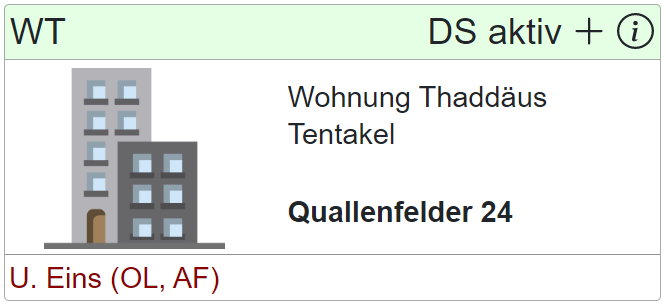
\includegraphics[width=.7\textwidth]{images/4-Feedback/objekt.png}
    \caption{Angepasste Darstellung von Objekten}
    \label{fig:feed-objekt}
\end{figure}

\textbf{Hintergrund von Objekten:} Ebenso wurde die Hintergrundfarbe von Objekten entfernt.
Hieraus resultiert eine bessere Lesbarkeit der Informationen, sowie eine gesteigerte Übersicht über alle Objekte, da die störenden Farbunterschiede wegfallen.

\textbf{Updates bearbeiten:} Updates können nun bearbeitet werden.
Hierzu kann auf das in \autoref{fig:feed-timeline} rechts zu sehende Stift-Symbol geklickt werden.
Danach ist der Text eines Updates editierbar, die Überschrift bleibt jedoch fest.
Gleichzeitig ändert sich der Stift in ein Hacken-Symbol.
Wird auf dieses geklickt, so wird der geänderte Text gespeichert und das Update kann nicht weiterbearbeitet werden.
Änderungen an einem Update werden erst im Moment des Klicks auf den Hacken mit der Datenbank synchronisiert.

\begin{figure}[htp]
    \centering
    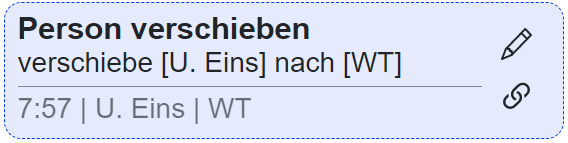
\includegraphics[width=.6\textwidth]{images/4-Feedback/timeline.png}
    \caption{Angepasste Darstellung von Updates}
    \label{fig:feed-timeline}
\end{figure}

\textbf{Timeline Tags:} Ebenso aus \autoref{fig:feed-timeline} zu erkennen ist eine neue Darstellung von Updates.
Zusätzlich zu Überschrift und Text findet sich unter diesen eine neue Zeile mit Informationen.
Hier werden die Zeit des Updates und alle in ihm erwähnten Personen, Objekte und andere Updates angezeigt.
Dieses Element fördert die Übersicht über die Timeline.
Ebenfalls eröffnet es die Möglichkeit für eine spätere tagspezifische Filterung der Timeline.

\textbf{Objekte Filtern:} Letztlich wurde die Benennung der Möglichkeit zum Filtern von Objekten angepasst.
Hier wird nun kein Filter mehr ausgewählt, es werden jedoch Tags hinzugefügt.
Damit soll den Nutzenden verdeutlicht werden, dass nur Objekte angezeigt werden, welche \textit{alle} gewählten Tags enthalten.
        \section{Erweiterungen}\label{sec:erweiterung}

\textbf{Einsatzleitung:} Die Darstellung der Einsatzleitung ist ebenfalls \autoref{fig:feed-objekt} zu entnehmen.
In dem in dieser Abbildung gezeigten Objekt liegt die Objektleitung beim Finanzamt.
Die Darstellung ist der klassischen Version nachempfunden, welche bereits in \autoref{sec:feedbackPerson} erklärt wurde.

Die momentane Darstellung ist jedoch nicht final.
Sie ist nur für Menschen mit konkretem Fachwissen zugänglich und sollte im Laufe der Zeit durch eine auch für Laien verständliche Version ersetzt werden.


\textbf{Zeiterfassung Protokoll:} Um die Zeit für ein Update genauer einstellen zu können wurde ein neuer Kontrollbereich eingeführt.
Dieser ist an der Stelle des Senden Knopfs im originalen Prototyp angesiedelt.
Zu sehen sind die Elemente für die Zeiteingabe in \autoref{fig:feed-time}.

\begin{figure}[htp]
    \centering
    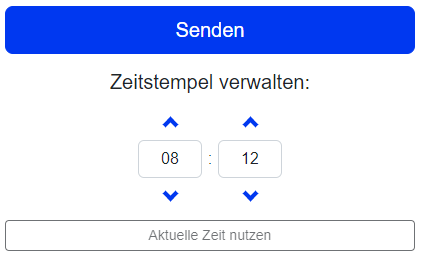
\includegraphics[width=.7\textwidth]{images/4-Feedback/time.png}
    \caption{Angepasste Eingabe der Updatezeit}
    \label{fig:feed-time}
\end{figure}

Dabei kann zwischen zwei Modi gewechselt werden.
Der als Standard ausgewählte Modus synchronisiert die Updatezeit stets mit der Systemzeit.
Hierzu wird die zu sehende digitale Uhr mit der aktuellen Uhrzeit synchronisiert.
Nach dem Absenden eines Updates wird die Zeit immer auf diese Einstellung zurückgesetzt.

Der zweite Modus kann für eine eigene Zeiteinstellung verwendet werden.
Hierzu kann die bestehende Uhrzeit entweder über die blauen Pfeile oder eine direkte Eingabe in die Eingabefelder geändert werden.
Sobald manuelle Änderungen an der Zeit festgestellt wurden wird die automatische Synchronisation gestoppt.
Möchten die Nutzenden zurück zur automatisiert synchronisierten Zeit zurückkehren, kann hierzu er untere Button "Aktuelle Zeit verwenden" geklickt werden.
Dieser ist nur aktiviert, solange die manuelle Zeiteingabe aktiv ist.

\textbf{Referenzieren von Updates:} Ebenfalls eingeführt wurde ein System zum Referenzieren von Updates.
Dieses ist jedoch auf eine Referenz pro Update beschränkt.
Wird auf den Link-Button in \autoref{fig:feed-timeline} geklickt, so wird dieses Update dem aktuellen Update als Referenz hinzugefügt.

\begin{figure}[htp]
    \centering
    
\includegraphics[width=\textwidth]{images/4-Feedback/reference.png}
    \caption{Referenzieren von Updates}
    \label{fig:feed-reference}
\end{figure}

Soll nun überprüft werden, welches Update momentan referenziert ist, kann auf die in \autoref{fig:feed-reference} zu sehenden Elemente geblickt werden.
Diese sind unter der Zeiteinstellung zu finden.
Das schwarz umrandete Feld zeigt dabei die Überschrift und die Zeit des referenzierten Updates an. Über den roten Button kann die Referenz entfernt werden.

\textbf{Letzte Standorte:} Dieses Feature wurde ebenfalls umgesetzt.
Dazu wird jeder verfügbaren Person in der Darstellung die Kennung ihres letzten Objekts in Klammern angehangen.

\textbf{Rechtschreibkorrektur:} Eine Rechtschreibkorrektur gestaltet sich als schwer umzusetzenden Feature.
Systeme für Rechtschreibkorrektur greifen stets auf Wortlisten zurück, welche auf externen Servern liegen.
Diese können aus dem internen Netzwerk des Finanzamts jedoch nicht angefragt werden.
Somit muss ein anderer Weg zur Umsetzung dieses Features gefunden werden.
Dies wurde jedoch auf einen späteren Zeitpunkt verlegt.
Vor Veröffentlichung der Software wird jedoch ein Rechtschreibkorrektur umgesetzt werden

    \chapter{Inclusive Design}\label{sec:incdes}

In diesem Kapitel wird der entwickelte Prototyp um Aspekte des Inclusive Design erweitert.
Hierzu wird die von Microsoft zur Verfügung gestellte Inclusive Design Toolbox \cite{ITToolkit} verwendet.

Im Folgenden wird deren Inhalt zunächst kurz zusammengefasst.
Dabei werden Aspekte des Inclusive Designs herausgearbeitet, welche daraufhin auf den bestehenden Prototypen angewendet werden.
Hierzu wird eine weitere Persona mit Beeinträchtigung vorgestellt, an deren Bedürfnisse der Prototyp angepasst wird.

Schlussendlich werden die Umgesetzten Ideen der Verbesserung bildlich präsentiert.
Sollten Anpassungen in bestimmten Bereichen nicht getätigt werden, so werden diese Entscheidungen begründet.
        \section{Erläuterung}

Dieser Abschnitt erläutert grundlegend die von Microsoft entwickelte Toolbox zum Thema Inklusive Design.
Dabei wird zunächst das Problem eingeschränkter Menschen mit vielen Anwendungen benannt.
Daraufhin werden Kontexte und Situationen benannt, in denen mit aufmerksamer Entwicklung Ausgrenzung vermieden werden kann.

\begin{quote}
"Eingeschränktheit entsteht an den Punkten der Interaktion zwischen Mensch und Gesellschaft.
Körperliche, kognitive und soziale Ausgrenzung ist das Ergebnis unangepasster Interaktionen." \cite{ITToolkit}
\end{quote}

Die Sicht auf körperliche Beeinträchtigungen als Fehler am Menschen ist veraltet.
An seine Stelle tritt eine neue Sicht, welche Beeinträchtigungen als kontextual begründet sieht.
Muss einem Rollstuhlfahrenden beim Einstieg in die Tram geholfen werden, so liegt dies nicht an der Person, sondern an einem fehlenden ebenerdigen Einstieg in das Transportmittel.
Ebenso verhält es sich im Gebiet der Softwareentwicklung.

Dabei wird zwischen drei Typen an Einschränkungen unterschieden:
Permanente Einschränkungen, wie beispielsweise ein amputierter Arm, Temporäre Einschränkungen, wie beispielsweise ein gebrochener Arm und Situative Einschränkungen, wie beispielsweise ein Elternteil, welches ein Baby im Arm trägt.
Oft wird Inklusion in der Software nicht umgesetzt, da ein hoher Aufwand in der Entwicklung nur einem kleinen Teil an Menschen zu Gute kommt.
Betrachtet man jedoch permanente, temporäre und situative Einschränkungen, so hilft jede inklusive Funktion mehr Menschen als im ersten Moment gedacht.

\subsection{Support Cards}

Um die Entwicklung von inklusiver Software zu unterstützen, hat Microsoft "Support Cards" entwickelt.
Diese behandeln jeweils Kontexte und Situationen, in denen Ausgrenzung auftreten kann.
Mit Hilfe der Karten können Entwickelnde prüfen, in welchem Umfang ihre Software inklusiv ist.
Diese Karten seien im Folgenden aufgelistet und kurz beschrieben.

\subsubsection{Physical Context}

Diese Karte regt die Entwickelnden an über das physische Umfeld potenzieller  Nutzenden nachzudenken.
Dabei sollte das Produkt möglichst an jedem Ort einsetzbar sein.
Es soll Zuhause am eigenen Schreibtisch, jedoch auch an anderen Orten, beispielsweise ohne Internet funktionieren.

\subsubsection{Social Context}

Ebenso soll das Produkt in jeglichen sozialen Kontexten einsetzbar sein.
Somit muss eine Einzelperson allein das Produkt bedienen können.
Gleichzeitig muss dies mit Kollegen oder Freunden und Familie funktionieren.
Ein letzter Punkt ist beispielsweise die Nutzung in einer Menschenmenge.
Hier ist die Nutzung beispielsweise durch Bewegungen und Lautstärke gestört.

\subsubsection{Temporary/Situational Limit}

Diese Karte bezieht sich auf Einschränkungen aller Art.
Dabei soll Software offen für Menschen sein, welche nicht sehen, sprechen, hören oder berühren können.
An diesem Punkt kommt ebenso die Beachtung von temporären und situativen Einschränkungen zum Tragen.
Eine Übersicht über einige Arten der Beeinträchtigung ist \autoref{fig:ways-of-disability} zu entnehmen.

\begin{figure}[htp]
    \centering
    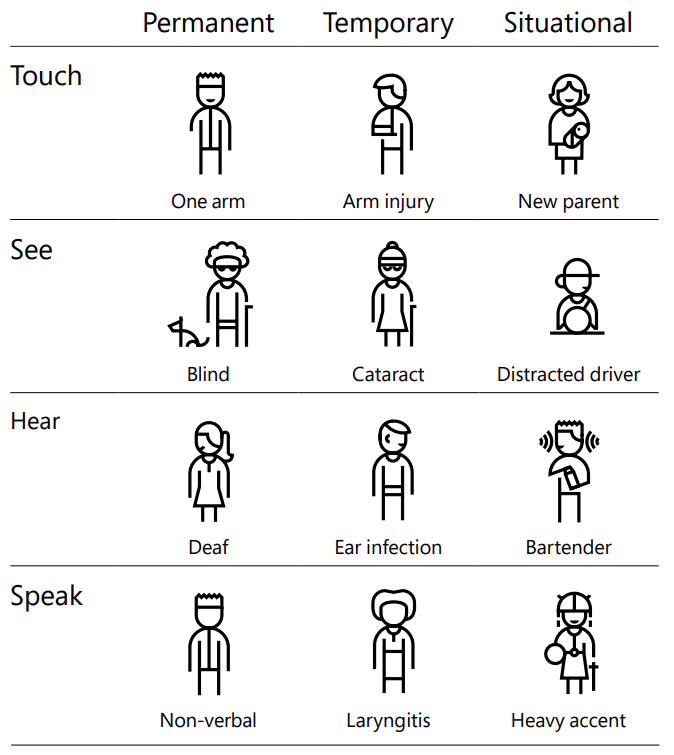
\includegraphics[width=.8\textwidth]{images/ID-disabilities.png}
    \caption{Arten von Eingeschränktheit \cite{ITToolkit}}
    \label{fig:ways-of-disability}
\end{figure}

\subsubsection{Role of Technology}

Wenn eine Software entwickelt werden soll, so soll diese eine Rolle einnehmen.
Beispielrollen sind Sammeln, Zusammenfassen, Übersetzen, Transportieren und Hören.
Im Zuge der Entwicklung sollen die Entwickler darauf achten, dass ihre Software die anfangs geforderte Rolle(n) einnimmt und nicht darüber hinaus arbeitet.
Dies steht in direkter Verbindung zu der in \autoref{sec:definition} erwähnten Aufgabenangemessenheit.

\subsubsection{Conditions}

Letztlich soll Software bei allen Bedingungen nutzbar sein.
Hierbei geht es beispielsweise um Wetter, Temperatur, aber auch Tageszeit.
Viele Nutzenden finden bei nächtlicher Arbeit beispielsweise das Angebot eines Blaufilters auf der Software für angemessen.


        \section{Zusätzliche Persona}

Um die Software im Folgenden in den Kategorien des Inklusive Designs testen zu können, wir zunächst eine weitere Persona erstellt.
Diese Persona verfügt über Eigenschaften, welche gewisse Barrierefreiheiten der Software voraussetzt.
Es wird nun zunächst die zusätzliche Persona, Lina Schneider, vorgestellt.
Daraufhin wird die Software mit Hilfe dieser und den Inklusive Design Support Cards \cite{ITToolkit} untersucht und an nötigen Stellen angepasst.

\autoref{fig:persona-lina} zeigt eine grafische Darstellung der Persona Lina Schneider.
Lina hat einen zweijährigen Sohn namens Jonas.
Nach der Elternzeit möchte sie nun wieder in ihren Job zurückkehren.
Ein Fahrradunfall, welcher einen gebrochenen Arm zu Folge hatte, erschwert ihr dies jedoch.
Da sie sich die Erziehung von Jonas mit ihrem Mann Moritz gut aufteilt, kann Lina trotz des Unfalls von Zuhause arbeiten.
Sie möchte trotz ihrer Einschränkungen an der Arbeit wie jede andere Person behandelt werden.

\begin{figure}[htp]
    \centering
    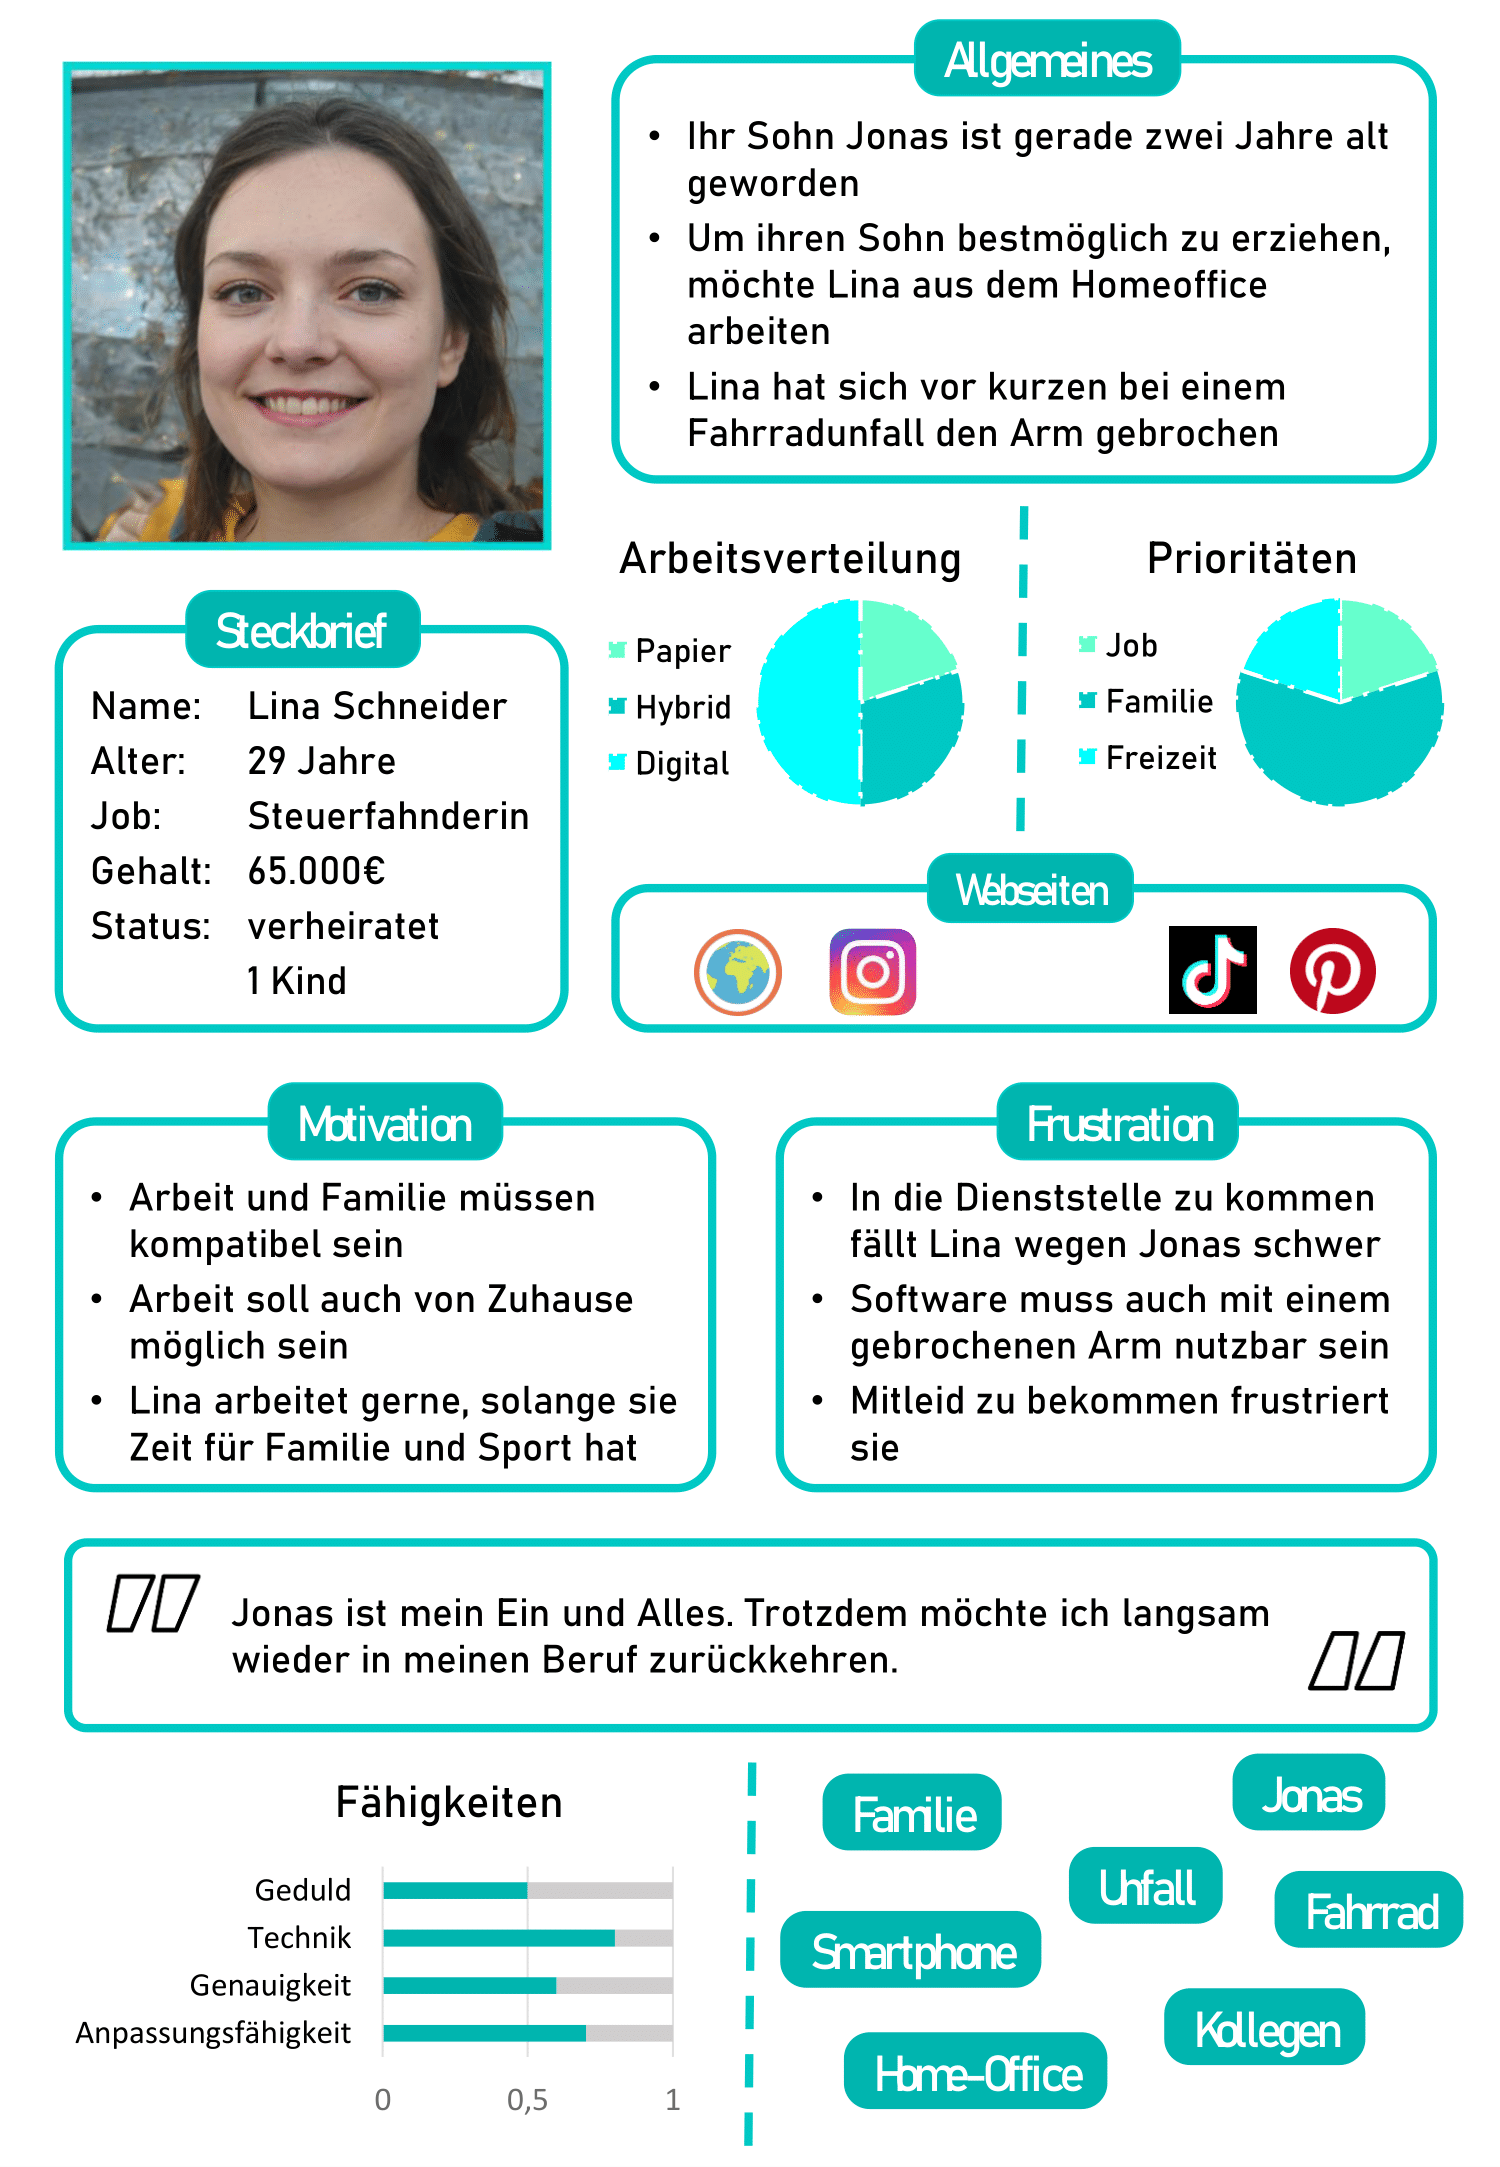
\includegraphics[width=\textwidth]{images/persona_2.png}
    \caption{Persona Lina Schneider}
    \label{fig:persona-lina}
\end{figure}
        \section{Anpassungen}

In diesem Abschnitt wird die Software mit Hilfe der Inklusive Design Support Cards \cite{ITToolkit} auf die Probe gestellt.
Dabei wird überlegt, welche Fälle bereits in der Software abgedeckt sind.
Ebenso wird für nicht abgedeckte Fälle überlegt, ob und wie diese von der Software abgedeckt werden können.

\subsubsection{Physical Context}

Der physikalische Kontext bezieht sich auf den Ort, an dem die Software eingesetzt wird.
Da es sich bei der Software um eine Arbeitsanwendung handelt, besitzt diese einen eingeschränkten Rahmen an Einsatzorten.

Primär wird sie mit den idealen Bildschirmgrößen in den Räumen des Finanzamts eingesetzt.
Soll jedoch die Persona Lina mit an einem Meldekopf teilhaben, so muss die Software auch auf einem einzigen Bildschirm im Home-Office funktionsfähig sein.
Dies ist gegeben.
Lina kann Eingabemaske und Übersichtsbildschirm in zwei separaten Tabs öffnen. 
Je nachdem welchen Tab sie benötigt, kann der andere Tab in den Hintergrund gestellt werden.

Als weiteren Einsatzort der Software ist in Zukunft der mobile Einsatz in Objekten oder im Auto zu nennen.
Perspektivisch soll der Digitale Meldekopf um eine Smartphone Version ergänzt werden.
Über diese können an der Durchsuchung beteiligte Personen über ihr Smartphone die aktuelle Timeline der Durchsuchung einsehen.
Das Eingeben von Informationen wird am Smartphone jedoch nicht möglich sein.
Hierzu ist zum aktuellen Zeitpunkt jedoch ebenso kein Anwendungsfall bekannt.

\subsubsection{Social Contex}

Die Problemstellung des sozialen Kontextes kann der digitale Meldekopf ebenfalls lösen.
Auch hier kommt ihm die Nutzung als Arbeitssoftware zu gute.
Die Benutzung mit Freunden, der Familie oder in einer Menschenmenge ist somit ausgeschlossen.
Des Weiteren kann die Software allein, oder im Team mit Kollegen genutzt werden.
Die alleinige Nutzung ist jedoch auf Grund der Menge an Arbeit im Zuge von Großdurchsuchungen nicht empfohlen.

\subsubsection{Temporary/Situational Limit}

Einschränkungen aller Art sind bei der Entwicklung von Software ein großes Thema.
Es muss entschieden werden, welche Einschränkungen von der Software unterstützt werden.
Nicht alle Einschränkungen werden vom Digitalen Meldekopf unterstützt.

Menschen ohne Sehvermögen können den Digitalen Meldekopf nur eingeschränkt bedienen.
Hierzu kann die von allen Betriebssystemen unterstützte Text-To-Speech Technologie verwendet werden.
Der geschriebene Inhalt wird den Nutzenden somit vorgelesen.
Eine Hilfe zu dieser Einschränkung enthält der Digitale Meldekopf jedoch nicht.
Durch den Einsatz der Text-To-Speech Technologie wird die Effizient des Digitalen Meldekopfs stark geschwächt.
Mit Hilfe geschickter Arbeitsteilung kann eine Erblindete Person jedoch ohne sinkende Effizienz in den Digitalen Meldekopf integriert werden.
Sie übernimmt den Telefonverkehr, während ein(e) Kolleg*in die Bedienung der Eingabemaske übernimmt.

Ist eine Stumme Person an Digitalen Meldekopf beteiligt, so kann ähnlich vorgegangen werden. 
Für das Nutzen der Software ist Sprache nicht notwendig.
So kann eine Stumme Person die Bedienung der Software übernehmen, während ein(e) Kolleg*in den Telefonverkehr übernimmt.
Selbes Vorgehen ist ebenfalls möglich, sollte eine Taube Person am Meldekopf teilhaben.

Sollte die Nutzung von Armen oder Händen einer Person eingeschränkt sein, so kann der Digitale Meldekopf nicht uneingeschränkt genutzt werden.
Das Eingeben von Informationen wird in allen Fällen durch eine sinkende Eingabegeschwindigkeit beeinträchtigt.
Über den Einsatz einer Speech-To-Text Technologie wurde nachgedacht.
Diese Technologien beziehen ihre Funktionalitäten jedoch von externen Servern.
Dies ist auf Grund der Vertraulichkeit der verarbeiteten Daten nicht erlaubt.
Eine Speech-To-Text Funktion kann also erst dann angeboten werden, wenn innerhalb der hessischen Finanzverwaltung ein solches Speech-To-Text Modell erstellt wird.

\subsubsection{Role of Technology}

Die Rollen des Digitalen Meldekopf sind das Sammeln und Zusammenfassen von Informationen, sowie ein Transport von Informationen zwischen Objekten und Meldekopf.
Diese Rollen erfüllt die vorgestellte Softwarelösung in allen Punkten.
An keiner Stelle findet die Bereitstellung unnützer Informationen statt.

\subsubsection{Conditions}

Des Weiteren Soll die Software bei unterschiedlichen Bedingungen genutzt werden.
Wetter und Temperatur tragen keinen Einfluss auf den Nutzen der Software.
Für Einsatzzeiten, zu denen des dunkel ist, ist zukünftig ein dunkler Modus geplant.
Dieser versucht die Oberfläche auch bei Dunkelheit für die Augen verträglich darzustellen.

Hier ebenso zu nennen sind Hintergrundgeräusche.
Diese treten beispielsweise bei der Persona Lina auf.
Bei anfallenden Hintergrundgeräuschen kann die Nutzung der Software durch Ablenkungen beeinträchtigt werden.
Dies kann jedoch durch das Verwenden von Kopfhörern vermieden werden.

    \chapter{Fazit}

Dieses abschließende Kapitel enthält ein Fazit zur Durchführung des nutzungsorientierten Prozesses am Beispiel des Digitalen Meldekopfs.
Zunächst folgen eine kurze Zusammenfassung und Rekapitulation des Prozesses.
Daraufhin ist eine Reflektion und kritische Auseinandersetzung mit der eigenen Arbeit zu finden.
Abschließend folgt ein Ausblick für das weitere Vorgehen im Projekt Digitaler Meldekopf.

In der kritischen Auseinandersetzung wird neben dem Ablauf des nutzungsorientierten Prozesses auch auf die konkrete Durchführung dieses eingegangen.
Dies ist nötig, da es in vielen Punkten nötig war, den Prozess zu Gunsten des Kontexts zu verändern.
Ebenso wird die Wahl des Digitalen Meldekopf als Kontext für diese Arbeit bewertet.
        \section{Zusammenfassung}

Die Durchführung des nutzungsorientierten Prozesses ist Zeitaufwendig.
Dies geht allein mit seiner Iterativen Definition einher.
Um diesen Aufwand abzuschwächen, wurde im Zuge dieser Arbeit auf Iterationen verzichtet und der nutzungsorientierten Prozesses in einen sequenziellen Rahmen gegossen.

Zu Beginn wurde in einem Interview im Kontext grundlegendes Wissen über den Kontext gewonnen.
Dieses Interview musste auf Grund des Kontextes methodisch angepasst werden.
Zwar wurde über fünf Stunden lang beobachtet, Fragen konnten jedoch erst am Ende gestellt werden.
Aus dem Interview im Kontext konnten Persona und IST-Szenario gewonnen werden.
Hierbei konnte die gelernte Methodik die vorgesehen angewandt werden.
Letztlich musste die Anzahl an Personas und Szenarien jedoch reduziert werden.

Im Zuge der Gestaltung des SOLL-Zustand konnten Gedanken und Fortschritte des zur selben Zeit bearbeiteten Semesterprojekt verwendet werden.
Somit konnte ein SOLL-Konzept schnell erarbeitet werden.
Das Verbessern dieses Konzepts begann mit einem Usability Test anhand zweier Prototypen.
Diese wurden nicht nur von der Kontextperson getestet.
In einem eine Großdurchsuchung begleitendem Versuch konnte der Autor seine eigene Software praktisch testen.
Da er selbst Erfahrungen in der Finanzverwaltung gesammelt hat, gehört dieser selbst in Teilen zu den potenziellen  Nutzenden.
Die in den Tests zu beanstandenden Funktionen wurden daraufhin verbessert und schlussendlich einer Überarbeitung im Rahmen des Inclusive Designs unterzogen.
        \section{Reflektion}

Der gewählte Kontext überschreitet den für diese Arbeit benötigten Umfang um ein weites.
Diese Erkenntnis wurde beim Zusammentragen der über das Semester gesammelten Informationen immer deutlicher.
Trotzdem wurde der nutzungsorientierte Prozess am Beispiel des Digitalen Meldekopf mit einer hohen Sorgfalt umgesetzt.

Jeder der getätigten Schritte forderte den Autor dabei auf eigene Weise.
Das Interview Im Kontext konnte zwar nicht direkt nach dem originalen Konzept ablaufen.
Trotzdem wurden die benötigten Informationen aus diesem gewonnen.
Die Gesamtzeit der Beobachtung im Laufe des Semesters betrug über 15 Stunden, aufgeteilt auf drei Großdurchsuchungen.
Dabei konnte Anfangs nur Auffälliges notiert werden.
In den späteren Durchsuchungen konnten bereits einige Konzepte und Ideen praktisch getestet werden.
Dadurch entstand eine Art ungewollte Iteration in der Entwicklung, welche jedoch nur den Entwickler selbst betraf.

Im Zuge der Rückmeldungen der Kontextperson wurde klar, dass trotz enormen in dieses Projekt geflossenem Aufwand nicht alle Ideen und Konzepte zielführend waren.
jedoch war es durch einen ausgezeichneten Austausch zwischen dem Entwickler und den Kontextpersonen möglich, jegliche Probleme und Wünsche in umsetzbare Konzepte umzuwandeln.
Es ist von Konzepten die Rede, da wie in \autoref{sec:erweiterung} zu erkennen ist, zum aktuellen Zeitpunkt nicht all diese Konzepte implementiert wurden.

Schlussendlich ist jedoch ein stark positiver Ausgang des nutzungsorientierten Prozesses festzuhalten.
Die durch ihn gewonnenen Informationen und Methoden haben großen Einfluss auch auf die Ausgestaltung der parallelen Projektarbeit.
Somit konnte der Autor nicht nur den durch NOG verursachten Mehraufwand spüren, sondern ebenfalls die aus diesem Aufwand resultierenden Früchte ernten.
Somit hat der nutzungsorientierte Prozess direkt eine sehr positive Auswirkung auf das Endprodukt.
        \section{Ausblick}

Abschließend sei erläutert, wie im Weiteren mit dem Digitalen Meldekopf verfahren wird.
Die Projektarbeit am Digitalen Meldekopf ist mit Ende dieses Semesters ebenfalls beendet.
Darauf aufbauend wir voraussichtlich im Sommersemester 2023 eine Bachlorarbeit über den Digitalen Meldekopf entstehen, im Zuge derer die Entwicklung vortgesetzt wird.
Ebenfalls wird der nutzungsorientierte Prozess fortgesetzt.
Hierzu wird nun in die dieses Semester übersprungene Iterationphase eingestiegen.

Im Zuge der Bachelorarbeit sollen bestehende Funktion weiter verbessert werden, es sollen jedoch auch neue Funktionen hinzugefügt werden.
Genauere Pläne liegen zu diesem Zeitpunkt jedoch nicht vor.
NOG soll jedoch in dieser Bachelorarbeit neben der Softwareentwicklung einen weiteren Einflussfaktor darstellen.

    % Die nächsten zwei Zeilen sind optional, sie sorgen dafür dass alles nach dem Inhalt wieder mit römischen Zahlen nummeriert wird.
    \pagenumbering{roman}
    \addtocounter{page}{3} % Dies ist die Anzahl der Seiten vor der Einleitung, muss möglicherweise angepasst werden, wenn das Inhaltsverzeichnis mehrere Seiten umfasst.

    \bibliographystyle{alphadin}
    \bibliography{main}

    \listoffigures
    % \listoftables
    \renewcommand{\listoflistingscaption}{Listing-Verzeichnis}
    % \listoflistings

    \appendix
    \chapter{Anhang}\label{ch:appendix}

\section{Checkliste Interview im Kontext}\label{ap:checkliste}

\begin{figure}[htp]
    \centering
    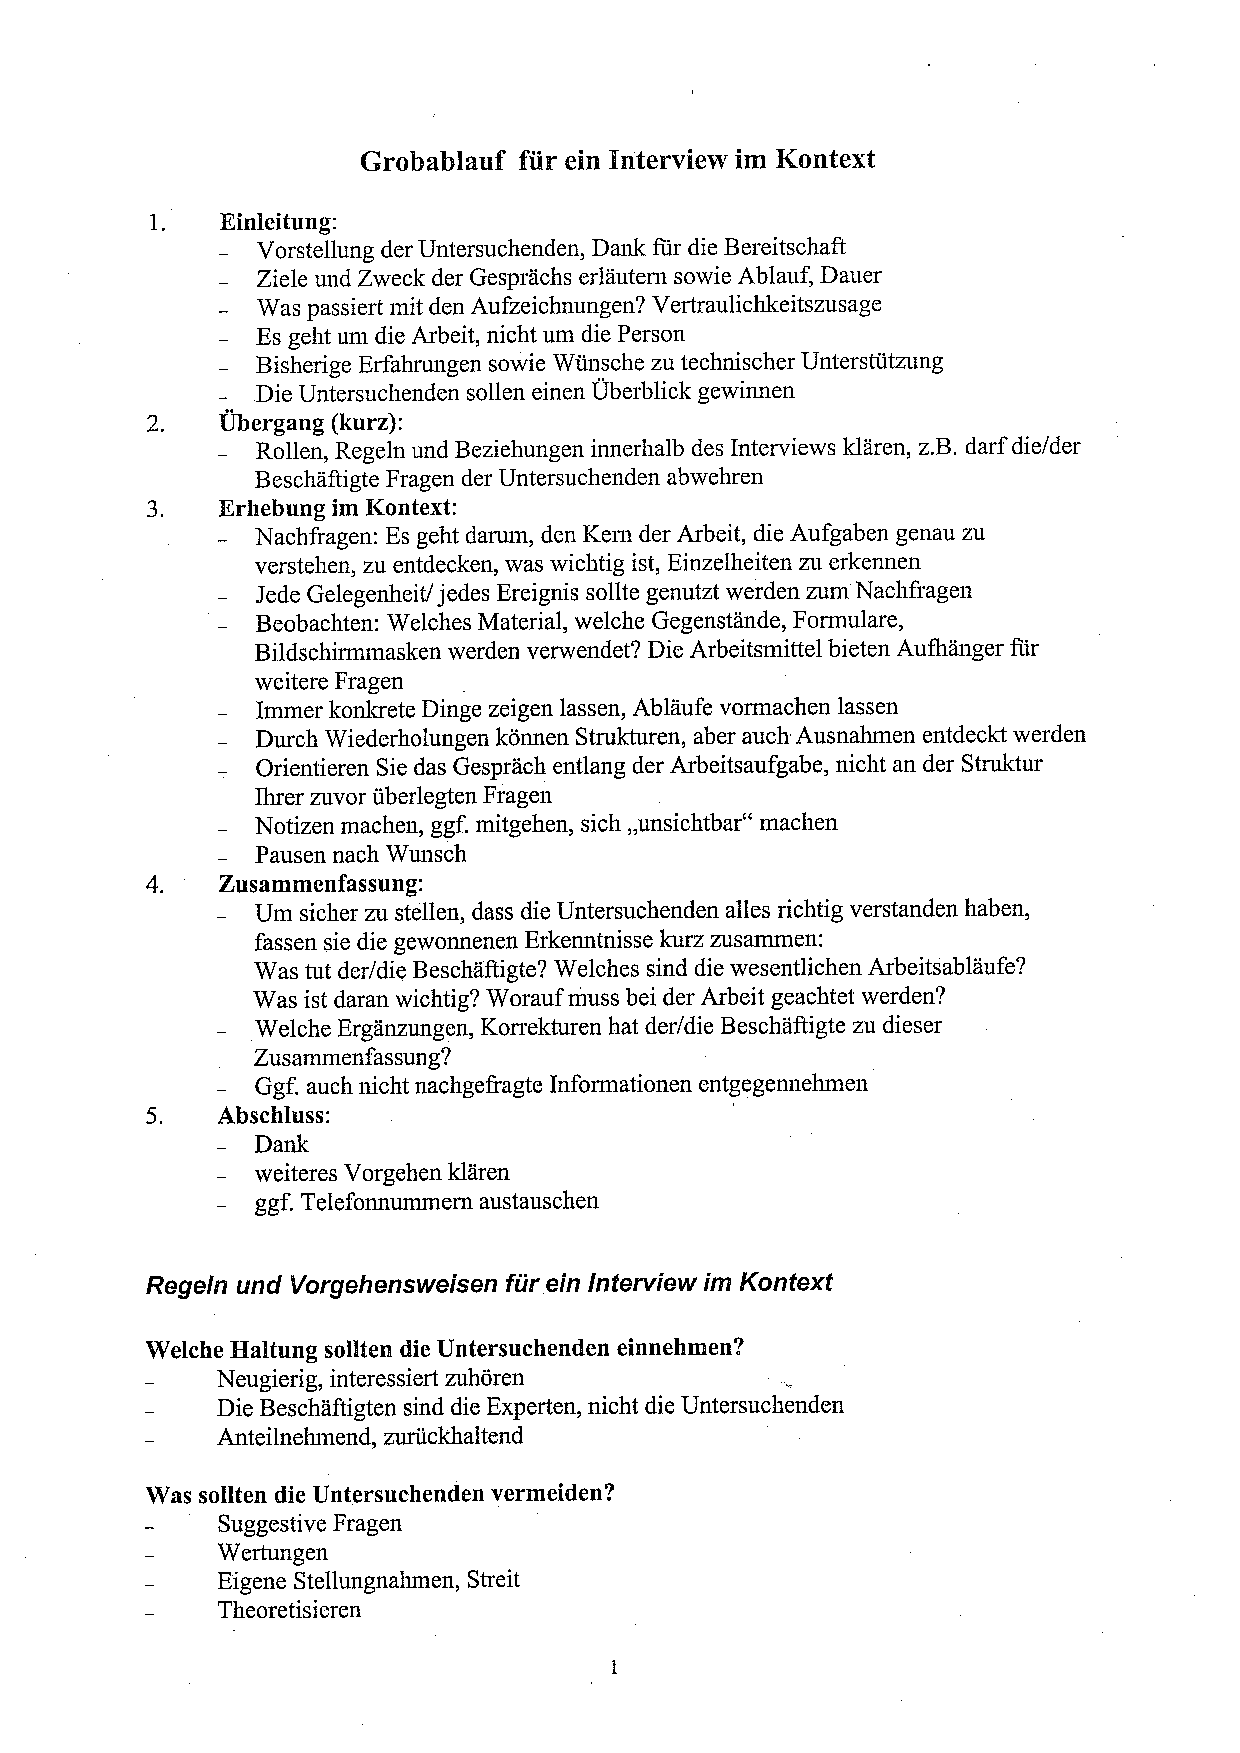
\includegraphics[width=.8\textwidth]{images/InterviewIK-Checkliste.pdf}
    \caption{Checkliste Interview im Kontext \cite{NOG}}
    \label{fig:IIK-Checkliste}
\end{figure}

\section{Darstellungen Persona}\label{ap:personas}

\begin{figure}[htp]
    \centering
    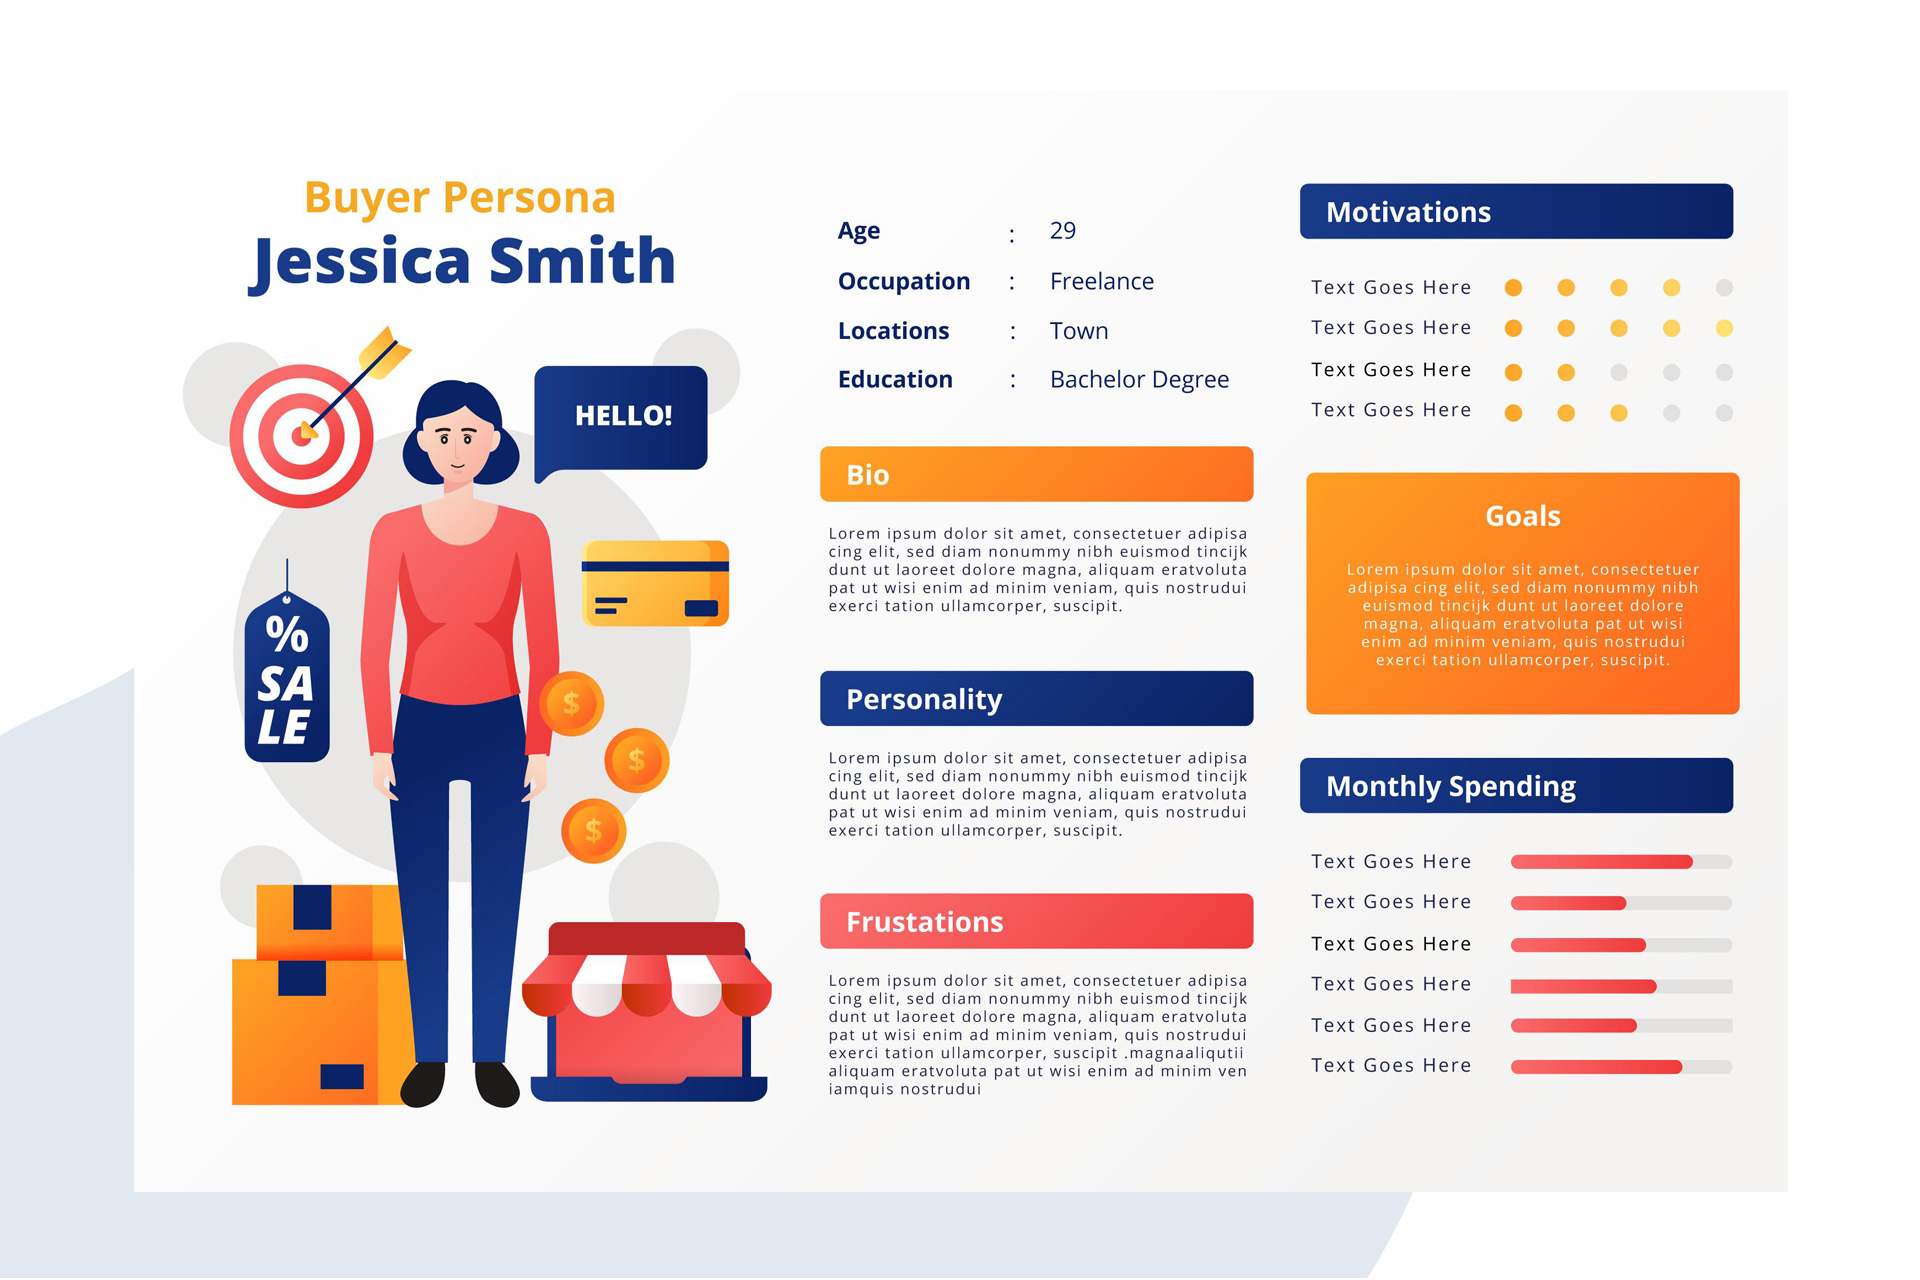
\includegraphics[width=\textwidth]{images/2-Personas/bspPersona1.jpg}
    \caption{Beispielpersona 1 \cite{captainverifyBuyerPersona}}
    \label{fig:bspPersona1}
\end{figure}

\begin{figure}[htp]
    \centering
    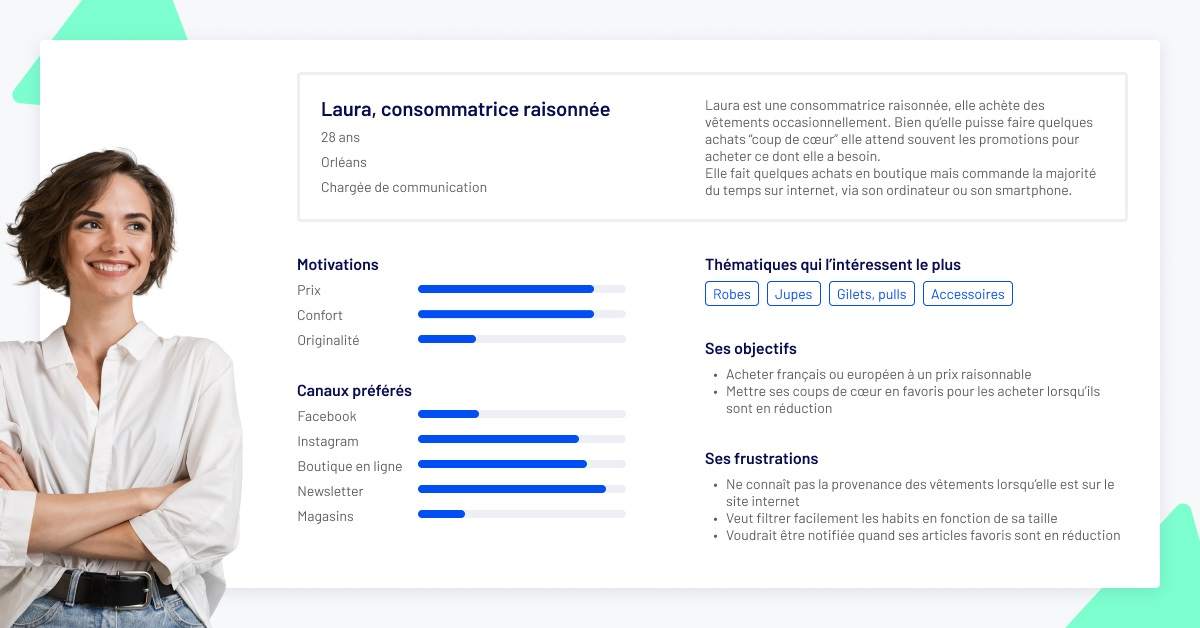
\includegraphics[width=\textwidth]{images/2-Personas/bspPersona2.jpg}
    \caption{Beispielpersona 2 \cite{interactiondesignWhatPersonas}}
    \label{fig:bspPersona2}
\end{figure}

\begin{figure}[htp]
    \centering
    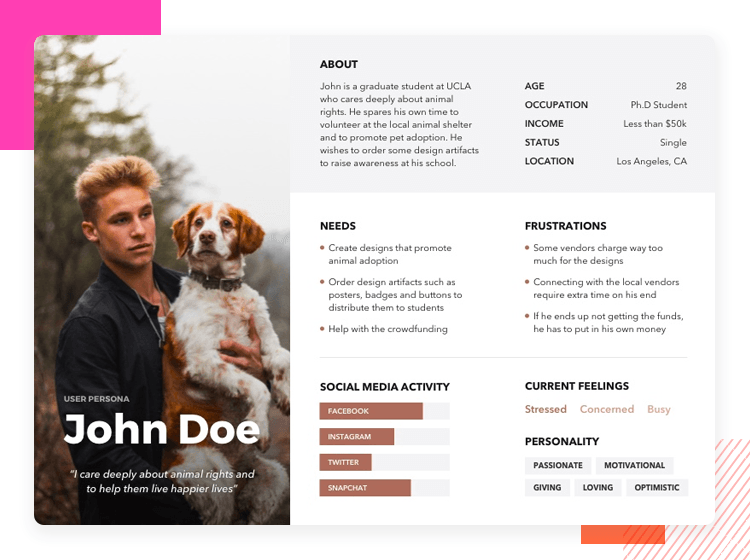
\includegraphics[width=\textwidth]{images/2-Personas/bspPersona3.jpg}
    \caption{Beispielpersona 3 \cite{uxplanetGuideCreating}}
    \label{fig:bspPersona3}
\end{figure}

    \chapter*{Eidesstattliche Erklärung}

% Inhaltsverzeichnis und Kopfzeile
% \addcontentsline{toc}{chapter}{Eidesstattliche Erklärung}
\markboth{Eidesstattliche Erklärung}{Eidesstattliche Erklärung}

Hiermit erkläre ich, dass ich die vorliegende Arbeit selbstständig und nur mit den nach der Prüfungsordnung der Universität Kassel zulässigen Hilfsmitteln angefertigt habe.
Die verwendete Literatur ist im Literaturverzeichnis angegeben.
Wörtlich oder sinngemäß übernommene Inhalte habe ich als solche kenntlich gemacht.

\vspace{1cm}

Kassel, \thesisdate

\begin{flushright}
  \underline{\hspace{7cm}} \\
  \thesisauthorname
\end{flushright}

\end{document}
